% !TeX encoding = UTF-8 Unicode
%% !TeX TS-program = make all
% !TeX TS-program = pdflatex
% !TeX root = report.tex
% !TeX spellcheck = en-GB
% !BIB program = bibtex
% MIT License - Copyright (c) 2021 Sergio Martínez-Losa
%
% IT IS MANDATORY TO HAVE TEX LIVE 2019 DISTRIBUTION INSTALLED TO COMPILE THIS TEMPLATE
%
%\documentclass[11pt,letterpaper,openright,spanish,english]{extbook}
%\documentclass[11pt,a4paper,spanish,english]{extbook}
\documentclass[11pt,a4paper,english]{book}
%\documentclass[11pt,a4paper,spanish,english]{book-unizar}
%\documentclass[11pt,a4paper,openright,spanish,english]{book}

\global\def\trueValue{true}
\global\def\falseValue{false}
\global\def\printabletext{true}
\global\def\printableimages{true}

\newcommand{\setprintabletext}[1]{
	
	\ignorespaces\lowercase{\def\tmp{#1}}\unskip
	
	\ifx\tmp\trueValue
		\global\def\printabletext{true}
	\else
		\global\def\printabletext{false}
	\fi
}

\newcommand{\setprintableimages}[1]{
	
	\ignorespaces\lowercase{\def\tmp{#1}}\unskip
	
	\ifx\tmp\trueValue
		\global\def\printableimages{true}
	\else
		\global\def\printableimages{false}
	\fi
}

\newcommand{\checkforceprintable}{
	
	\ifdefined\forceprint
		\setprintabletext{true}
		\setprintableimages{true} 
	\else
		\setprintabletext{false}
		\setprintableimages{false} 
	\fi
}

\newif\iftwoside
\twosidetrue

\newcommand{\twosidelayout}[1][]{
	
	\ignorespaces\lowercase{\def\tmp{#1}}\unskip

	\ifx\tmp\empty
		\twosidetrue
	\else
	
		\ifx\tmp\falseValue
			\twosidefalse
		\else
			\twosidetrue
		\fi
	\fi
}

\newcommand{\onesidelayout}{\twosidelayout[false]}

% set document title
\global\def\THETITLE{Harmony Is All You need}

% set document author
\global\def\THEAUTHOR{Tin Ferković, Dorian Smoljan}

% set document university
\global\def\THEUNIVERSITY{University of Zagreb}

% set faculty name
\global\def\THEFACULTY{Faculty of Electrical Engineering and Computing}

% ser PhD programme
\global\def\THEPHDPROGRAMME{Physics PhD Program}


% Set whether twoside enable of not (true or false), by default twoside
%\twosidelayout[true] % select twoside layout
\twosidelayout[false] % select oneside layout
%\twosidelayout % default twoside layout active
%\onesidelayout % equivalent to \twosidelayout[false]

\checkforceprintable

\usepackage[utf8]{inputenc}
\usepackage[main = english, spanish]{babel}
\usepackage{float}
\usepackage{booktabs}
\usepackage[a4paper,margin=2.2cm]{geometry}
%\usepackage[letterpaper,margin=2.2cm]{geometry}
%\usepackage[pdftex]{graphicx} %% loaded twice
\usepackage[nodayofweek]{datetime}
\usepackage[labelfont=bf]{caption}
\usepackage{acronym}
\usepackage[normalem]{ulem}
\usepackage{enumitem}
\usepackage{amsmath}
\usepackage{amssymb}
\usepackage{extarrows}
\usepackage[makeroom]{cancel} % cross-out terms in equations
\usepackage{subfig}
\usepackage{xifthen}
\usepackage{twoopt}
\usepackage{wasysym}
\usepackage{fancyhdr}
\usepackage{siunitx}
\usepackage{fix-cm} % mandatory for Package cover 
\usepackage{titlesec} % mandatory for Package cover 
\usepackage[T1]{fontenc} % mandatory for Package cover 
\usepackage{adjustbox} % mandatory for alt colour cover
\usepackage[biblabel, nomove]{cite} % citation package and style -> https://tex.stackexchange.com/questions/79591/superscripts-in-bibliography-with-bibtex#79599
\usepackage[protrusion=true,expansion]{microtype} % install cm-super -> https://tex.stackexchange.com/questions/88368/how-do-i-invoke-cm-super#88374
%\usepackage[activate={true,nocompatibility},final,tracking=true,kerning=true,spacing=true,factor=1100,stretch=10,shrink=10]{microtype}
%\usepackage{lmodern}

\ifx\printabletext\trueValue
	%\usepackage[monochrome]{xcolor}
	\PassOptionsToPackage{monochrome}{xcolor}
	\relax
\else
	%\usepackage[dvipsnames, table]{xcolor}
	\relax
	\PassOptionsToPackage{dvipsnames, table}{xcolor}
	%\usepackage{color, colortbl}
\fi

\ifdefined\mainmatter
	\usepackage{tocbasic} % mainmatter style book
	\usepackage{xpatch} % mainmatter style book
\fi

\usepackage{morewrites} % https://www.ctan.org/pkg/morewrites
\usepackage[none]{hyphenat} % do not split words at the en of line
\usepackage{afterpage}
\usepackage{xfrac} % diagonal fractions --> https://tex.stackexchange.com/questions/3372/how-do-i-typeset-arbitrary-fractions-like-the-standard-symbol-for-5-%C2%BD
\usepackage{newfloat} % float environment for equation listing
\usepackage[subfigure]{tocloft}
\usepackage{etoolbox}
\usepackage{everyshi}
\usepackage{atbegshi}
\usepackage{atveryend}
\usepackage{yfonts}
\usepackage{todonotes}
\usepackage{tikz}
\usetikzlibrary{shapes.geometric, calc}
\usepackage[siunitx, RPvoltages]{./packages/circuitikzgit}
\usepackage{anyfontsize}
\usepackage{minted}
\usepackage{array}
\usepackage[column=O, math]{cellspace}
\usepackage{makecell} % https://tex.stackexchange.com/questions/558937/how-to-avoid-broken-horizontal-and-vertical-lines-when-using-multirow-and-multic
\usepackage{multirow}
\usepackage[bottom]{footmisc}
%\usepackage[printwatermark]{xwatermark}
%\usepackage{everypage}
%\usepackage{./packages/bibspacing}
\usepackage{hyperref}
\usepackage{glossaries} % always load glossaries AFTER hyperref
\usepackage{ifplatform}
\usepackage[linesnumbered,ruled]{algorithm2e}
%\usepackage{catoptions}
%\usepackage{menukeys}
\usepackage{csquotes} % https://tex.stackexchange.com/questions/120722/how-to-modify-a-bibliography-style-to-surround-titles-in-quotes-in-a-bibliograph
% https://tex.stackexchange.com/questions/64761/add-just-a-little-more-padding-to-my-table/381439
\cellspacetoplimit 4pt

% space after figures
%\setlength{\belowcaptionskip}{-5pt}

\iftwoside
    \relax
	\typeout{@@@}
	\typeout{@@@ SELECTED TWO-SIDE}
	\typeout{@@@}
	
	\makeatletter
		\@twosidetrue
	\makeatother
\else
    \relax
	\typeout{@@@}
	\typeout{@@@ SELECTED ONE-SIDE}
	\typeout{@@@}
	
	\makeatletter
		\@twosidefalse
	\makeatother
\fi

\newif\iffilepublications

% set true or false to view the list of publications 
\filepublicationstrue

\iffilepublications

	\makeatletter
		\@ifpackageloaded{multibib}{\relax}{
			\usepackage[resetlabels]{multibib} % multiple bibliography
		}
	\makeatother

\fi

\newif\ifnotwindows

\ifwindows
	% do nothing
	\relax
\else
	\notwindowstrue
\fi

\newcommand{\ConfigLinksBlack}{
	
	\hypersetup{
		colorlinks = true,
		linkcolor=black,
		citecolor=black,
		filecolor=black,
		urlcolor=black,
		runcolor=black,
		menucolor=black,
		linkbordercolor=black,
		citebordercolor=black,
		filebordercolor=black,
		urlbordercolor=black,
		runbordercolor=black,
		menubordercolor=black,
		pdfpagemode=UseOutlines,
		hypertexnames = true,
		pdfencoding = auto, 
		psdextra, 
		bookmarksdepth = 4
		bookmarks=true,
		bookmarksopen=true,    
		bookmarksopenlevel=0,
		bookmarksnumbered=true,
		plainpages=false
	}
}

\newcommand{\ConfigLinksColours}{

	% style color setup: https://tex.stackexchange.com/questions/525261/better-default-colors-for-hyperref-links
	
	\definecolor{blue-hyperref}{rgb}{0,0.2,0.6}
	
	\hypersetup{
		colorlinks = true,
		linkcolor=blue-hyperref,
		citecolor=blue-hyperref,
		filecolor=blue-hyperref,
		urlcolor=blue-hyperref,
		runcolor=blue-hyperref,
		menucolor=blue-hyperref,
		linkbordercolor=blue-hyperref,
		citebordercolor=blue-hyperref,
		filebordercolor=blue-hyperref,
		urlbordercolor=blue-hyperref,
		runbordercolor=blue-hyperref,
		menubordercolor=blue-hyperref,
		pdfpagemode=UseOutlines,
		hypertexnames = true,
		pdfencoding = auto, 
		psdextra, 
		bookmarksdepth = 4
		bookmarks=true,
		bookmarksopen=true,    
		bookmarksopenlevel=0,
		bookmarksnumbered=true,
		plainpages=false
	}
	
%	\hypersetup{
%		colorlinks = true
%		,linkcolor=NavyBlue %BrickRed
%		,citecolor=Green
%		,filecolor=Mulberry
%		,urlcolor=NavyBlue
%		,menucolor=BrickRed
%		,runcolor=Mulberry
%		,linkbordercolor=BrickRed
%		,citebordercolor=Green
%		,filebordercolor=Mulberry
%		,urlbordercolor=NavyBlue
%		,menubordercolor=BrickRed
%		,runbordercolor=Mulberry
%	}
}

\ifx\printabletext\trueValue

	\ConfigLinksBlack

\else
	
	\ifdefined\compileblack
	
		\ConfigLinksBlack
	
	\else
	
		\ConfigLinksColours
	
	\fi
\fi

\ifx\printabletext\trueValue
	\typeout{@@@}
	\typeout{@@@ PRINTING BLACK AND WHITE TEXT}{}
	\typeout{@@@}
\else
	\typeout{@@@}
	\typeout{@@@ PRINTING RGB TEXT}{}
	\typeout{@@@}
\fi

\ifx\printableimages\trueValue
	\typeout{@@@}
	\typeout{@@@ PRINTING BLACK AND WHITE IMAGES}{}
	\typeout{@@@}
\else 
	\typeout{@@@}
	\typeout{@@@ PRINTING RGB IMAGES}{}
	\typeout{@@@}
\fi

% https://tex.stackexchange.com/questions/525261/better-default-colors-for-hyperref-links

%\hypersetup{
%	colorlinks = true,
%	linkcolor={[rgb]{0,0.2,0.6}},
%	citecolor={[rgb]{0,0.6,0.2}},
%	filecolor={[rgb]{0.8,0,0.8}},
%	urlcolor={[rgb]{0.8,0,0.8}},
%	runcolor={[rgb]{0.8,0,0.8}},  % defaults to filecolor but it missing an
%	% expansion for this syntax
%	menucolor={[rgb]{0,0.2,0.6}}, % I never set or use this, so we'll see
%	% it to link color
%	linkbordercolor={[rgb]{0,0.2,0.6}},
%	citebordercolor={[rgb]{0,0.6,0.2}},
%	filebordercolor={[rgb]{0.8,0,0.8}},
%	urlbordercolor={[rgb]{0.8,0,0.8}},
%	runbordercolor={[rgb]{0.8,0,0.8}},
%	menubordercolor={[rgb]{0,0.2,0.6}},
%	hypertexnames=false 
%}

%\hypersetup{
%	colorlinks = true,
%	linkcolor = {[rgb]{0,0.2,0.6}},
%	anchorcolor = {[rgb]{0,0.2,0.6}},
%	citecolor = {[rgb]{0,0.2,0.6}},
%	filecolor = {[rgb]{0,0.2,0.6}},
%	urlcolor = {[rgb]{0,0.2,0.6}},
%	hypertexnames=false
%}

%\hypersetup{
%	colorlinks = true,
%	linkcolor = blue,
%	anchorcolor = blue,
%	citecolor = blue,
%	filecolor = blue,
%	urlcolor = blue,
%	hypertexnames=false
%}

% space in glossary entries, bibspacing
%\setlength{\bibitemsep}{.2\baselineskip plus .05\baselineskip minus .05\baselineskip}

% PDF compression parameters: https://latex.org/forum/viewtopic.php?t=21309
\pdfminorversion=5
\pdfcompresslevel=9
\pdfobjcompresslevel=2
\pdfinclusioncopyfonts=1

\typeout{@@@ pdfcompresslevel=\the\pdfcompresslevel}
\typeout{@@@}
\typeout{@@@ pdfobjcompresslevel=\the\pdfobjcompresslevel}
\typeout{@@@}
\typeout{@@@ pdfminorversion=\the\pdfminorversion}
\typeout{@@@}

\DeclareGraphicsExtensions{.png,.pdf}

\newcommand{\keywords}{physics, resume, summary, report, phd, magnonics, quantum, simulations}

% https://tex.stackexchange.com/questions/48067/pdfinfo-doesnt-appear-to-be-working#48070
\ifpdf
	\makeatletter
		\AtBeginDocument{
			\hypersetup{
				pdftitle={\@title~\expandonce\THETITLE},
				pdfauthor={\@author},
				pdfkeywords={\keywords},
				pdfproducer={\expandonce\THEAUTHOR},
				pdfcreator={\expandonce\THEAUTHOR},
				pdfsubject={\expandonce\THETITLE},
				pdfinfo={
					Title={\THETITLE},
					Author={\THEAUTHOR},
					Creator={\THEAUTHOR},
					Producer={\THEAUTHOR}
				}
			}
		}
	\makeatother
\fi

\setlist[itemize]{itemsep=0.005cm}

\newif\ifformat
\formattrue

% Command to avoid style expand in TOC/LOT/LOF
\newcommand{\donotexpandstyles}[1]{
	\AtBeginDocument{\addtocontents{#1}{\protect\formatfalse}}
	\AtEndDocument{\addtocontents{#1}{\protect\formattrue}}
}

% Do not expand styles in table of contents
\donotexpandstyles{toc}
% Do not expand styles in list of tables
\donotexpandstyles{lot}
% Do not expand styles in list of figures
\donotexpandstyles{lof}
% Do not expand styles in list of equations
\donotexpandstyles{equ}

% Do not show styles on TOC/LOT/LOF, put \maybe before styled text
\makeatletter
\DeclareRobustCommand{\maybe}[1]{%
	\ifformat
		\expandafter#1%
	\else
		\expandafter\@firstofone
	\fi
}
\makeatother

% remove word Chapter at the beginning of each chapter
%\titleformat{\chapter}[block]{\normalfont\huge\bfseries}{\thechapter.}{1em}{\Huge}\titlespacing*{\chapter}{0pt}{-19pt}{0pt}
% https://tex.stackexchange.com/questions/62516/how-to-suppress-chapter-in-chapter-while-keeping-numbering
\makeatletter
\def\@makechapterhead#1{%
	\vspace*{-19\p@}%
	{\parindent \z@ \raggedright \normalfont
		\ifnum \c@secnumdepth >\m@ne
			\if@mainmatter
				%\huge\bfseries \@chapapp\space \thechapter
				\Huge\bfseries \thechapter.\space%
				%\par\nobreak
				%\vskip 20\p@
			\fi
		\fi
		\interlinepenalty\@M
		\Huge \bfseries #1\par\nobreak
		\vskip 10\p@
}}
\makeatother

\ifx\printableimages\trueValue
%	\immediate\write18{chmod +x utils/convert-grayscale.sh && ./utils/convert-grayscale.sh &>/dev/null}
	\graphicspath{{./images-grayscale/}}
\else
	\graphicspath{{./images/}}
\fi

% Continous footnote counter
% https://tex.stackexchange.com/questions/10448/continuous-footnote-numbering
\counterwithout{footnote}{chapter}

%% INDENTATION REVIEW
\newif\ifindentfirst
\newif\ifindentall

\indentfirstfalse
\indentallfalse

\def\indentspace{\hspace*{1em}}
\def\noindentspace{\hspace*{0em}}

\ifindentfirst

	% START INDENT ONLY FIRST PARAGRAPH OTHER PARAGRAPHS NOT INDENT

	\makeatletter
	\def\@afterheading{%
		\@nobreaktrue
		\everypar{%
			\if@nobreak
				\@nobreakfalse
				\clubpenalty \@M
				\indentspace%
			\else
				\clubpenalty \@clubpenalty
				\everypar{}%
			\fi}}
	\makeatother
	\setlength{\parindent}{0pt}

	% END INDENT ONLY FIRST PARAGRAPH OTHER PARAGRAPHS NOT INDENT

\else

	\ifindentall
	
		\setlength{\parindent}{1em}
		
	\else
	
		%% START NOT INDENT FIRST PARAGRAPH OTHER PARAGRAPHS INDENT
		
		\makeatletter
		\def\@afterheading{%
			\@nobreaktrue
			\everypar{%
				\if@nobreak
					\@nobreakfalse
					\clubpenalty \@M
					\noindentspace%
				\else
					\clubpenalty \@M
					\indentspace
				\fi}}
		\makeatother
		\setlength{\parindent}{0em}
		
		%% END NOT INDENT FIRST PARAGRAPH OTHER PARAGRAPHS INDENT
	
		%% PATCH INDENT AFTER ENVIRONMENT LIST BASED
		% https://tex.stackexchange.com/questions/112404/reliable-code-for-automatic-noindent-after-specific-environments
		% https://tex.stackexchange.com/questions/23062/an-unexpected-value-of-clubpenalty
		
		\makeatletter
		\let\nearly@afterheading\@afterheading
		\patchcmd\nearly@afterheading
			{\@M} % original temporary setting for \clubpenalty replaced by ...
			{\@clubpenalty\protect\indentspace} % ... or whichever value you deem right
			{}{}
	
		\newcommand*\IndentAfterEnv[1]{%
			\AfterEndEnvironment{#1}{\par\@afterindentfalse\nearly@afterheading}}
		
		\newcommand*\SpaceBeforeEnv[1]{%
			\BeforeBeginEnvironment{#1}{\par\protect\vspace*{0.5em}}}
		\makeatother

		% indent after environment
		\IndentAfterEnv{itemize}
		\IndentAfterEnv{enumerate}
		
		% mandatory for a \parskip of 0.7em
		\SpaceBeforeEnv{itemize}
		\SpaceBeforeEnv{enumerate}
		
		%% END PATCH INDENT AFTER ENVIRONMENT LIST BASED
	\fi

\fi
%% END INDENTATION REVIEW

%% START TOC STYLE
% https://tex.stackexchange.com/questions/154646/is-there-an-easy-way-to-get-the-frontmatter-mainmatter-and-backmatter-in-a-l/154666
% https://tex.stackexchange.com/questions/419555/remove-bold-style-for-chapter-names-in-table-of-contents
% https://tex.stackexchange.com/questions/123774/remove-the-dots-next-to-chapter-in-memoir
% https://tex.stackexchange.com/questions/299074/removing-number-on-toc-but-maintaining-the-position-of-the-text
% http://www.texfaq.org/FAQ-isdef

\ifdefined\mainmatter

	% https://tex.stackexchange.com/questions/439926/different-style-for-backmatter-chapters-in-toc
	% \mainmatter defined
	\typeout{@@@@@@@@@@@@@}
	\typeout{@@@@@@@@@@@@@ mainmatter defined}
	\typeout{@@@@@@@@@@@@@}
	
	\DeclareTOCStyleEntry[entryformat=\chapterentryformat,pagenumberformat=\chapterentryformat]{tocline}{chapter}
	
	\newif\ifmainmatterintoc
	
	\newcommand*\chapterentryformat[1]{{\ifmainmatterintoc\normalfont\bfseries\else\normalfont\slshape\fi#1}}
	
	\xapptocmd\mainmatter{\addtocontents{toc}{\protect\mainmatterintoctrue}}{}{\mmPatchFailed}
	\xapptocmd\backmatter{\addtocontents{toc}{\protect\mainmatterintocfalse}}{}{\appPatchFailed}

\else

	% \mainmatter not defined
	\typeout{@@@@@@@@@@@@@}
	\typeout{@@@@@@@@@@@@@ mainmatter NOT defined}
	\makeatletter
	\typeout{@@@@@@@@@@@@@}
	
	\newcommand*{\enableboldchapterintoc}{%
		
		\addtocontents{toc}{\protect\unexpanded{\protect\unexpanded{\string\renewcommand{\protect\cftchapdotsep}{\protect\cftnodots}}}} % remove dots
		\addtocontents{toc}{\string\renewcommand{\protect\cftchapfont}{\protect\normalfont\protect\bfseries}}
		\addtocontents{toc}{\string\renewcommand{\protect\cftchappagefont}{\protect\normalfont\protect\bfseries}}
		\addtocontents{toc}{\string\renewcommand{\protect\cftchapleader}{\protect\bfseries\hfill\relax}}
		%	\addtocontents{toc}{\string\renewcommand{\protect\cftchapleader}{\protect\bfseries\protect\cftdotfill{\protect\cftsecdotsep}}} % dot leaders in bold
	}
	
	\newcommand*{\enableitalicchapterintoc}{%
		
		\addtocontents{toc}{\protect\unexpanded{\protect\unexpanded{\string\renewcommand{\protect\cftchapdotsep}{\protect\cftnodots}}}} % remove dots
		\addtocontents{toc}{\string\renewcommand{\protect\cftchapfont}{\protect\normalfont\protect\itshape}}
		\addtocontents{toc}{\string\renewcommand{\protect\cftchappagefont}{\protect\normalfont\protect\itshape}}
		\addtocontents{toc}{\string\renewcommand{\protect\cftchapleader}{\protect\itshape\hfill\relax}}
	}
	
	\newcommand*{\disablestylechapterintoc}{%
		
		\addtocontents{toc}{\string\renewcommand{\protect\cftchappagefont}{\protect\normalfont}}
		\addtocontents{toc}{\string\renewcommand{\protect\cftchapfont}{\protect\normalfont}}
		\addtocontents{toc}{\string\renewcommand{\protect\cftchapleader}{\protect\normalfont\protect\cftdotfill{\protect\cftsecdotsep}}}% 
	}
	
	\newcommand{\frontmatter}{%
		
		\disablestylechapterintoc
		\enableitalicchapterintoc
		
		\cleardoublepage
		\pagenumbering{Roman}
	}
	
	\newcommand{\mainmatter}{%
		
		\disablestylechapterintoc
		\enableboldchapterintoc
		
		\cleardoublepage
		\pagenumbering{arabic}
	}
	
	\newcommand{\backmatter}{%
		
		\disablestylechapterintoc
		\enableitalicchapterintoc
		
		\if@openright
			\cleardoublepage
		\else
			\clearpage
		\fi
	}
	
	\makeatother

\fi

%% END TOC STYLE

% https://tex.stackexchange.com/questions/323455/bold-math-in-title-but-not-in-toc
\newcommand\AvoidBoldMathInTocFor[1]{
	\titleformat*{#1}{\bfseries\boldmath}
}

\AvoidBoldMathInTocFor{\section}
\AvoidBoldMathInTocFor{\subsection}
\AvoidBoldMathInTocFor{\subsubsection}

% Check twoside or oneside document
\makeatletter
% https://tex.stackexchange.com/questions/360785/how-do-i-check-if-a-document-is-oneside-or-twoside#360791
\if@twoside%

    \relax
	\typeout{@@@@@@@@@@@@@}
	\typeout{@@@@@@@@@@@@@ TWO-SIDE DOCUMENT}
	\typeout{@@@@@@@@@@@@@}
	
	% CLEAN DOUBLE PAGES ON TWOSIDE MODE
	% https://tex.stackexchange.com/questions/62572/twoside-introduces-incorrect-linespacing-at-end-of-section
	\raggedbottom
	% https://stackoverflow.com/questions/491904/how-do-i-remove-blank-pages-coming-between-two-chapters-in-appendix
	\let\cleardoublepage\clearpage
	% END CLEAN DOUBLE PAGES ON TWOSIDE MODE
	
\else%
    \relax
	\typeout{@@@@@@@@@@@@@}
	\typeout{@@@@@@@@@@@@@ ONE-SIDE DOCUMENT}
	\typeout{@@@@@@@@@@@@@}
	
\fi%  

\makeatother

% brakets for citation superscripts
% https://tex.stackexchange.com/questions/79591/superscripts-in-bibliography-with-bibtex#79599
\makeatletter 
	\renewcommand{\@citess}[1]{\textsuperscript{\,[#1]}} 
\makeatother

% https://tex.stackexchange.com/questions/29084/biblatex-separator-for-citing-multiple-sources-some-of-them-with-page-some-no
%\renewcommand\multicitedelim{\addcomma\space}

% cell spaces global
% https://tex.stackexchange.com/questions/378268/makegapedcells-disables-rowcolor#378630
\setlength\cellspacetoplimit{4pt}
\setlength\cellspacebottomlimit{4pt}

\ifx\printabletext\trueValue
	\relax
\else
	% change colour of glossary links
	% https://tex.stackexchange.com/questions/38544/glossary-links-color
	\def\glossarylinknewcolour{orange}
	
	\ifdefined\compileblack
		\def\glossarylinknewcolour{black}
	\else
		\def\glossarylinknewcolour{orange}
	\fi

	\makeatletter
	
		\newcommand{\glsplainhyperlink}[2]{\colorlet{currenttext}{\glossarylinknewcolour}\colorlet{currentlink}{\@linkcolor}\hypersetup{linkcolor=currenttext}\hyperlink{#1}{#2}\hypersetup{linkcolor=currentlink}}
		\let\@glslink\glsplainhyperlink
		
	\makeatother
\fi


% set paragraph spacing
\setlength{\parskip}{0.7em}

% renew commands

\renewcommand\thepage{\romannumeral\numexpr\value{page}-1\relax}

% rework glossary title
%\renewcommand{\glossarypreamble}{\vspace*{\baselineskip}\vspace*{\parskip}}

% rework glossary title (better)
\renewcommand{\glossarypreamble}{\vspace{-1.5cm}{\flushright\rule{\linewidth}{1pt}\vspace*{3ex}}\protect\thispagestyle{phdfancyempty}}

\renewcommand{\arraystretch}{1.2}

% glossary custom style: 
% https://tex.stackexchange.com/questions/327328/glossaries-style-change-add-units
\newglossarystyle{betterglossary}{%
	\setglossarystyle{list}%

	\renewcommand*{\glossentry}[2]{%

		\item[\glsentryitem{##1}\glstarget{##1}{\glossentryname{##1}\normalfont{:}}]

		\glossentrydesc{##1}. ##2
	}%

	\renewcommand*{\glsgroupskip}{}%
}

% Renew the glossary entry command to be always uppercase
% mfirstuc – Uppercase the first letter of a word
\renewcommand{\glsnamefont}[1]{\makefirstuc{#1}}

% REMOVE INDENTATION DESCRIPTION ENVIRONMENT GLOSSARY
% https://stackoverflow.com/questions/49843733/change-hanging-indentation-for-latex-description-environment
\makeatletter
\renewenvironment{description}%
{\list{}{\leftmargin=0pt % <------- Adjust this length
		\labelwidth\z@ \itemindent-\leftmargin
		\let\makelabel\descriptionlabel}}%
{\endlist}
\makeatother

%\renewcommand because amssymb package has a command called \bold
\renewcommand{\bold}[1]{\textbf{#1}}

% system modifications
 
\setlength{\heavyrulewidth}{0.07em}
\newcommand{\otoprule}{\midrule[\heavyrulewidth]}

\newdateformat{monthyeardate}{\monthname[\THEMONTH] \THEYEAR}
\newcommand{\monthtoday}{\date{\monthyeardate\today}}

% https://tex.stackexchange.com/questions/112932/today-month-as-text
\newdateformat{coverdate}{\monthname[\THEMONTH] \THEYEAR}

% new commands
\newcommand{\matrixbraket}[2]{
	$\begin{pmatrix}
	#1 \\
	#2 \\
	\end{pmatrix}$
}

\newminted{mumax3}{frame=lines,framerule=2pt}

\newcommand{\newquote}[1]{``#1''}

\newcommand{\italic}[1]{\textit{#1}}

\newcommand{\fixheaderbadness}{
	\hbadness=10000 % A parameter that tells TeX at what point to report badness errors (i.e. underfull and overfull error). [number] ranges from 0 to 10000. 
	\vbadness=10000 % A parameter that tells TeX at what point to report badness errors (i.e. underfull and overfull error). [number] ranges from 0 to 10000. 
	\hfuzz=100pt % A parameter that allows hbox's to be overfull by [length] before an overfull error occurs. 
	\pretolerance=10000
}

\newcommand{\newchapter}[2]{
	
	\protect\chapter{#1}
	\label{#2}
	\setlength{\parsep}{\parskip}%
}

\newcommand{\centerItem}[1]{
	
	\begin{center}
		#1
	\end{center}
}

\newcommand{\imagefigurecaption}[4][0.35]{
	
	\begin{figure}[H]
		\centering
		\includegraphics[width=#1\textwidth,height=\textheight,keepaspectratio]{#2}
%		\captionsetup{justification=centering}
		\captionsetup{belowskip=\spaceBelowCaptionFigures, justification=raggedright, singlelinecheck=true}
		\caption{#3}
		\ifthenelse{\equal{#4}{}}{}{\label{#4}}
	\end{figure}	
}

\newcommand{\imagefigure}[3][0.35]{
	
	\imagefigurecaption[#1]{#2}{#3}{}	
}

% https://tex.stackexchange.com/questions/37581/latex-figures-side-by-side
\newcommand{\asideimages}[9][false]{
	
	\begin{figure}[H]
		
		% if captions from subfire are empty, remove the marker below the image
		\ifthenelse{\equal{#5}{}}{
			\ifthenelse{\equal{#7}{}}{
				%				\captionsetup[subfigure]{labelformat=empty}
				\captionsetup[subfigure]{belowskip=\spaceBelowCaptionFigures, labelformat=empty, justification=raggedright, singlelinecheck=true}
			}{}
		}{}
		
		\centering
		\subfloat[#5]{
			{\includegraphics[width=#2]{#4}}
		}
		\qquad
		\subfloat[#7]{
			{\includegraphics[width=#3]{#6}}
		}
		
		\ignorespaces\lowercase{\def\tmpVal{#1}}
		
		\ifthenelse{\equal{\tmpVal}{false}}{
			\centercaption{#8}
		}{	
			\nocitecentercaption{#8}
		}
		
		\label{#9}
		
	\end{figure}
}

\newcommand{\gridimages}[12][false]{%
    \begin{figure}[H]
        \centering
        
        % if captions are empty, remove the marker below the image
        \ifthenelse{\equal{#5}{}}{%
            \ifthenelse{\equal{#7}{}}{%
                \captionsetup[subfigure]{belowskip=\spaceBelowCaptionFigures, labelformat=empty, justification=raggedright, singlelinecheck=true}%
            }{}%
        }{}%
        
        \begin{minipage}{0.45\textwidth}
            \centering
            \includegraphics[width=\linewidth]{#4}
            \caption{#5}
            \label{fig:subfig1}
        \end{minipage}%
        \hfill%
        \begin{minipage}{0.45\textwidth}
            \centering
            \includegraphics[width=\linewidth]{#6}
            \caption{#7}
            \label{fig:subfig2}
        \end{minipage}
        
        \vspace{0.5cm}
        
        \begin{minipage}{0.45\textwidth}
            \centering
            \includegraphics[width=\linewidth]{#8}
            \caption{#9}
            \label{fig:subfig3}
        \end{minipage}%
        \hfill%
        \begin{minipage}{0.45\textwidth}
            \centering
            \includegraphics[width=\linewidth]{#10}
            \caption{#11}
            \label{fig:subfig4}
        \end{minipage}
        
        \ignorespaces\lowercase{\def\tmpVal{#1}}%
        
        \ifthenelse{\equal{\tmpVal}{false}}{%
            \centercaption{#12}
        }{%
            \nocitecentercaption{#12}
        }
        
        \label{#13}
        
    \end{figure}
}

% used to avoid caption cite in LOF
\newcommand{\asideimagesnocite}[8]{
	\asideimages[true]{#1}{#2}{#3}{#4}{#5}{#6}{#7}{#8}
}

\newenvironment{changemargin}[2]{%
	
	\begin{list}{}{%
			\setlength{\topsep}{3pt}%
			\setlength{\leftmargin}{#1}%
			\setlength{\rightmargin}{#2}%
			\setlength{\listparindent}{\parindent}%
			\setlength{\itemindent}{\parindent}%
			\setlength{\parsep}{\parskip}%
		}%
	\item[]}{\end{list}}
	
\def\spaceBelowCaptionFigures{-10pt}
\def\spaceBelowCaptionEquations{-2pt}

\newcommand{\centercaptionequation}[1]{	
	%	\captionsetup{justification=centering}
	\captionsetup{belowskip=\spaceBelowCaptionEquations, justification=raggedright, singlelinecheck=true}
	\protect\caption{#1}
}
	
\newcommand{\centercaption}[1]{	
%	\captionsetup{justification=centering}
	\captionsetup{belowskip=\spaceBelowCaptionFigures, justification=raggedright, singlelinecheck=true}
	\protect\caption{#1}
}

\newcommand{\nocitecentercaption}[1]{	
	%	\captionsetup{justification=centering}
	\captionsetup{belowskip=\spaceBelowCaptionFigures, justification=raggedright, singlelinecheck=true}
	\protect\nocitecaption{#1}
}

\newcommand{\centercaptionlisting}[1]{
%	\captionsetup{justification=centering}
	\captionsetup{belowskip=\spaceBelowCaptionFigures, justification=raggedright, singlelinecheck=true}
	\protect\caption[#1]{\boldmath{#1}}
}

\DeclareCaptionType{equ}[][]

% https://tex.stackexchange.com/questions/39315/how-to-change-the-numbering-for-different-figures
\newcommand{\equationname}{Equation}
\DeclareFloatingEnvironment[name={\protect\equationname}]{eqfigure}

\newcommand{\setequation}[5] {
	
	\begin{equ}[H]
		
		% https://tex.stackexchange.com/questions/316646/renaming-the-label-of-figure-just-in-some-cases
		%		\renewcommand{\figurename}{Equation}
		\begin{changemargin}{#1}{#2}
			\begin{eqfigure}[H]
				#3
				\vspace{-0.5cm}
				\centercaptionequation{#5}
				\label{#4}
				\addequations{#5} % this is for equations listing
			\end{eqfigure}
		\end{changemargin}	
		\vspace{-1.5cm}
	\end{equ}
}

\newcommand{\setequationboxed}[6] {
	
	\begin{equ}[H]
		% https://tex.stackexchange.com/questions/316646/renaming-the-label-of-figure-just-in-some-cases
		%		\renewcommand{\figurename}{Equation}
		\begin{changemargin}{#1}{#2}
			\begin{eqfigure}[H]
				#3
				\vspace{#6}
				\centercaptionequation{#5}
				%				\centercaptionformula{#5}
				\label{#4}
				\addequations{#5} % this is for equations listing
			\end{eqfigure}
		\end{changemargin}
		\vspace{-1.5cm}
	\end{equ}
}

\newcommand{\centerformula}[1]{
	\vspace{-0.8cm}
	\begin{align}
		#1
	\end{align}
}

\newcommand{\tpower}[1]{
	\ensuremath{\times\ 10^{#1}}
}

\newcommand{\super}[1]{\textsuperscript{#1}}

\newcommand{\sub}[1]{\textsubscript{#1}}

% better diameter symbol
\DeclareFontEncoding{LS1}{}{}
\DeclareFontSubstitution{LS1}{stix}{m}{n}
\DeclareRobustCommand{\diameter}{%
	\text{\usefont{LS1}{stixscr}{m}{n}\symbol{"60}}%
}

\global\def\enableTODO{true}

\newcommand{\showtodos}[1] {
	\global\def\enableTODO{#1}
}

\definecolor{amber}{rgb}{1.0, 0.75, 0.0}

\definecolor{red-clean}{rgb}{1.0, 0.41, 0.38}

\definecolor{red}{rgb}{1,0,0}

\definecolor{amber}{rgb}{1.0, 0.75, 0.0}

\definecolor{red-light}{rgb}{1.0, 0.41, 0.38}

\definecolor{blue-light}{rgb}{0.58, 0.86, 1}

\newcommand{\TODO}[1]{
	\def\trueOption{true}
	\ifx\enableTODO\trueOption
		\ifx\printableimages\trueValue
			\todo[inline, shadow=0.8, bordercolor=black, color=white]{\qquad\bold{TODO}: #1}
		\else
			\todo[inline, shadow=0.8, bordercolor=black, color=red!50]{\qquad\bold{TODO}: #1}
		\fi
	\fi
}

\makeatletter
\newcommandtwoopt{\sticker}[3][][true]{%
	
	\ignorespaces\lowercase{\def\valueTmp{#1}}
	\ignorespaces\lowercase{\def\indentStatusParagraph{#2}}

	\def\itemWidth{long}
	
	\ifx\printableimages\trueValue
	
		\ifx\valueTmp\itemWidth
			\todo[inline, shadow=0.8, bordercolor=black, color=white]{\qquad#3}
		\else
			\todo[inline, shadow=0.8, bordercolor=black, color=white]{\qquad\centerline{#3}}
		\fi
		
	\else
	
		\ifx\valueTmp\itemWidth
			\todo[inline, shadow=0.8, bordercolor=black, color=amber!50]{\qquad#3}
		\else
			\todo[inline, shadow=0.8,bordercolor=black, color=amber!50]{\qquad\centerline{#3}}
		\fi
		
	\fi
	
	\ifx\indentStatusParagraph\trueValue
		\par\@afterindentfalse\@afterheading % avoid indent on first paragraph after TODO note
	\fi
	% https://tex.stackexchange.com/questions/229001/do-not-indent-second-paragraph-after-macro-was-used
}
\makeatother


\makeatletter

\newcommandtwoopt{\stickerMultiline}[3][amber!50][true] {

		% Set true if TODO note is right below the title else set false on #2
		\ignorespaces\lowercase{\def\valueTmp{#2}}
		\ignorespaces\lowercase{\def\valueBackColourTmp{#1}}
		
		\ifx\printableimages\trueValue
			\ignorespaces\lowercase{\def\valueBackColourTmp{white}}
		\fi 

		\if\valueTmp\trueValue
		
			\todo[inline, shadow=0.8, bordercolor=black, color=\valueBackColourTmp]{#3}
			% check if user sets the TODO right below title or not
			\par\@afterindentfalse\@afterheading % avoid indent on first paragraph after TODO note
			
		\else
		
			\@nobreaktrue
			\todo[inline, shadow=0.8, bordercolor=black, color=\valueBackColourTmp]{#3}
			\@nobreakfalse
			
		\fi
}

\makeatother

% https://tex.stackexchange.com/questions/40561/table-with-multiple-lines-in-some-cells
\newcommand{\celltwolines}[2]{%

	\begin{tabular}{@{}c@{}}
		#1 \\ #2
	\end{tabular}
}

%% WATERMARK STUFF
%Customize watermark
%\global\def\optionWatermark{true}
%
%\newcommand{\docwatermark}[1]{
%	
%	\global\def\optionWatermark{#1}
%	\newsavebox\mybox
%	\savebox\mybox{\tikz[color=gray,opacity=0.3,font=\sffamily]\node{#1};}
%	\newwatermark*[allpages,angle=45,scale=10,xpos=-30,ypos=15]{\usebox\mybox}
%}
%
%\newcommand{\showwatermark}[2]{
%	
%	\def\constPreliminary{PRELIMINARY}
%	\def\truestr{true}
%	\ignorespaces\lowercase{\def\tmp{#1}}\unskip
%	\def\valueNull{\par}
%	
%	\ifx\tmp\valueNull
%		\docwatermark{\constPreliminary}
%		\global\def\optionWatermark{true}
%	\else
%		\ifx\tmp\truestr
%			\ignorespaces\def\optValue{#2}\unskip
%	
%			\ifx\optValue\valueNull
%				\docwatermark{\constPreliminary}
%			\else
%				\def\voidValue{}
%				\ifx\optValue\voidValue
%					\docwatermark{\constPreliminary}
%				\else 
%					\docwatermark{\uppercase{#2}}
%				\fi
%			\fi
%	
%			\global\def\optionWatermark{true}
%		\else
%%		\fi
%	\fi
%}

\newcommand{\preliminary}[2]{
	
	\showwatermark{#1}{#2}
}

\newcommand{\showpreliminary}[2]{
	
	\showwatermark{#1}{#2}
}

\newcommand{\gothicletter}[2][black]{
	
	\yinipar{\color{#1}#2}\hspace{-0.5em}
}

\newcommand{\changeTitleDocument}[1]{
	
	\ignorespaces\lowercase{\def\tmp{#1}}\unskip
	
	\ifx\tmp\empty
		% value empty, nothing to do
	\else
		\global\def\THETITLE{#1}
	\end
}

% rework toc, lot and lof title, add line below
\renewcommand{\cftaftertoctitle}{\\\rule{\linewidth}{1pt}\vspace*{3ex}}
\renewcommand{\cftafterlottitle}{\\\rule{\linewidth}{1pt}\vspace*{3ex}}
\renewcommand{\cftafterloftitle}{\\\rule{\linewidth}{1pt}\vspace*{3ex}}

% rework bibliography title
% https://tex.stackexchange.com/questions/70025/titlesec-and-bibliography
% https://latex.org/forum/viewtopic.php?t=28709
\newcommand{\SetTitleBibliography}[1]{
	\renewcommand{\bibname}{#1}
}

\newcommand{\titlebibliography}[1]{
	\addto{\captionsenglish}{\bibname}
}

\def\customquad{\hskip\baselineskip\relax}

\patchcmd{\thebibliography}{\chapter*{\bibname}}{\chapter*{\flushleft\bibname\vspace{-0.6cm}\customquad\rule{\linewidth}{1pt}\vspace{-0.5cm}}\protect{\thispagestyle{phdfancyempty}}}{}{}

% redefine plain style to empty style
% https://tex.stackexchange.com/questions/65089/im-trying-to-redefine-the-plain-pagestyle-as-empty
\makeatletter
\let\ps@plain\ps@empty
\makeatother

% create new chapter without page reference in TOC, optional, to set an horizontal line below the title
% create new chapter without page reference in TOC, optional, to set an horizontal line below the title
\newcommandtwoopt{\chaptercustompageintoc}[4][showrule][true]{
	
	% https://tex.stackexchange.com/questions/50038/suppress-page-numbers-when-using-addcontentsline
	\ifthenelse{\equal{#1}{showrule}}{
		
		\chapter*{\flushleft#3\vspace{-0.5cm}\customquad\rule{\linewidth}{1pt}\vspace{-1.2cm}}
		
	}{
		
		\chapter*{\flushleft{#3}\vspace{-0.5m}\customquad}
	}
	
	\ifthenelse{\equal{#2}{true}}{
		\cftaddtitleline{toc}{chapter}{#3}{#4}
	}
}

% plain pagestyle
\newcommandtwoopt{\chapterpagenumberintoc}[3][showrule][true] {
	
	\ifthenelse{\equal{#1}{showrule}}{
		
		\chapter*{\flushleft#3\vspace{-0.6cm}\customquad\rule{\linewidth}{1pt}\vspace{-1.2cm}}
	}{
		
		\chapter*{\flushleft{#3}\vspace{-0.6cm}\customquad}
	}
	
	\ifthenelse{\equal{#2}{true}}{
		\addcontentsline{toc}{chapter}{#3}
	}
}
%% input file for abstract

\global\def\showpageabstract{false}
\global\def\showrule{showrule}
\global\def\showintoc{true}

\newcommandtwoopt{\inputabstract}[4][false][showrule]{
	
	\ignorespaces\lowercase{\def\tmp{#1}}
	\global\def\showpageabstract{\tmp}
	
	\ignorespaces\lowercase{\def\tmprule{#2}}
	\global\def\showrule{\tmprule}
	
	% whether or not to show in TOC
	\ignorespaces\lowercase{\def\tmptoc{#3}}
	\global\def\showintoc{\tmptoc}
	
	\ifthenelse{\equal{\tmp}{false}}{
		
		% abstract without page numbers and without page number in TOC
		\protect\pagestyle{empty}\input{#4}
		\protect\thispagestyle{empty}
	}{
		
		% abstract with page numers and page number in TOC
		\protect\pagestyle{phdfancyempty}\input{#4}
		\protect\thispagestyle{phdfancyempty}
	}
	
	\clearpage
}

\newcommand{\abstractname}{Abstract}

\newcommand{\inputabstracttitle}{
	
	\ifthenelse{\equal{\showpageabstract}{false}}{

		\chaptercustompageintoc[\showrule][\showintoc]{\abstractname}{}		
	}{
	
		\chapterpagenumberintoc[\showrule][\showintoc]{\abstractname}
	}
}

%% end input file for abstract

% environment for justified text
\newenvironment{justified}[1] {
	\setlength\parindent{0pt}
	\setlength{\parsep}{\parskip}%
	#1
}{}

% environment italic text
\newenvironment{shapeitalic} {
	\itshape
}{}

%% START Create a list of equations

% https://tex.stackexchange.com/questions/270611/creating-list-of-equations
\newcommand{\equationpagetext}{Page}
\newcommand{\listequationsname}{List of Equations}
\newcommand{\listequationtitle}{\vspace{-0.4cm}\listequationsname\vskip0cm\vspace{-0.59cm}\rule{\linewidth}{1pt}\vspace{1.8cm}\\\protect{\hspace*{0pt}\hfill\fontsize{11}{12}\textbf{\equationpagetext}\par\protect\thispagestyle{phdfancyempty}\vspace{-1.0cm}}}
\newlistof{addequations}{equ}{\listequationtitle}
\newcommand{\addequations}[1]{%
	\addcontentsline{equ}{addequations}{\protect\numberline{\theeqfigure}#1}\par}
\addtolength{\cftaddequationsnumwidth}{13pt}
\setlength{\cftaddequationsindent}{1.5em}
\setlength{\cftaddequationsnumwidth}{2.3em}

%% END Create a list of equations

% change default color to superscript footnote
% https://tex.stackexchange.com/questions/26693/change-the-color-of-footnote-marker-in-latex
\makeatletter

\ifdefined\compileblack
	\def\footnotecolour{\color{black}}
\else
	\def\footnotecolour{\color{red-clean}}
\fi

\renewcommand\@makefnmark{\hbox{\@textsuperscript{\normalfont\footnotecolour\@thefnmark}}}
\renewcommand\@makefntext[1]{%
	\parindent 1em\noindent
	\hb@xt@1.8em{%
		\hss\@textsuperscript{\normalfont\@thefnmark}}#1}
\makeatother

%% START List of Publications 

% USE multibib package: https://www.overleaf.com/learn/latex/Multibib
% https://tex.stackexchange.com/questions/170316/nocite-for-single-bibdatasources-with-biblatex-biber
% https://www.privacypies.org/blog/2017/01/25/bib-management.html
\newcommand{\listofpublicationsname}{List of Publications}

%% END List of Publications

\newcommand{\tikzimagefigure}[2]{

	\begin{figure}[H]
		\centering
		#1
%		\captionsetup{justification=centering}
		\captionsetup{belowskip=\spaceBelowCaptionFigures, justification=raggedright, singlelinecheck=true}
		\caption{#2}
	\end{figure}
}

\newcommand{\tikzimagefigurelabel}[3]{

	\begin{figure}[H]
		\centering
		#2
%		\captionsetup{justification=centering}
		\captionsetup{belowskip=\spaceBelowCaptionFigures, justification=raggedright, singlelinecheck=true}
		\caption{#3}
		\ifthenelse{\equal{#1}{}}{}{\label{#1}}
	\end{figure}
}

% Change the page numbering style and continue with the page counter
% https://tex.stackexchange.com/questions/453254/continue-previous-page-numbering-roman-arabic-with-two-independent-counters
% #1 -> Choose the numbering style: Arabic, Roman, etc.
% #2 -> Choose variable holding the page number, default buit-in variable named "page"
\newcommandtwoopt{\ContinuePaginingWithNumbering}[2][arabic][page] {

	\newcounter{savepagetoken}
	\setcounter{savepagetoken}{\value{#2}}
	\pagenumbering{#1}
	\setcounter{#2}{\value{savepagetoken}}
}

% change colour of glossary links
% https://tex.stackexchange.com/questions/38544/glossary-links-color
%\def\glossarylinknewcolour{orange}
%
%\makeatletter
%\newcommand{\glsplainhyperlink}[2]{\colorlet{currenttext}{\glossarylinknewcolour}\colorlet{currentlink}{\@linkcolor}\hypersetup{linkcolor=currenttext}\hyperlink{#1}{#2}\hypersetup{linkcolor=currentlink}}
%\let\@glslink\glsplainhyperlink
%\makeatother

% Fix space TOC/LOT/LOF
% https://tex.stackexchange.com/questions/69321/spacing-between-chapters-in-list-of-tables
\makeatletter

\def\@chapter[#1]#2 {
	
	\ifnum\c@secnumdepth > \m@ne
		\if@mainmatter
			\refstepcounter{chapter}%
			\typeout{\@chapapp\space\thechapter.}%
			\addcontentsline{toc}{chapter}{\protect\numberline{\thechapter}#1}%
		\else
			\addcontentsline{toc}{chapter}{#1}%
		\fi
	\else
		\addcontentsline{toc}{chapter}{#1}%
	\fi
	
	\chaptermark{#1}%
	%                    \addtocontents{lof}{\protect\addvspace{10\p@}}% NEW
	%                    \addtocontents{lot}{\protect\addvspace{10\p@}}% NEW
	\if@twocolumn
		\@topnewpage[\@makechapterhead{#2}]%
	\else
		\@makechapterhead{#2}%
		\@afterheading
	\fi
}

\makeatother

% Make subsubsubsections available
% https://tex.stackexchange.com/questions/60209/how-to-add-an-extra-level-of-sections-with-headings-below-subsubsection
% https://tex.stackexchange.com/questions/186981/is-there-a-subsubsubsection-command
\newif\ifexpandsubsublevel

\expandsubsublevelfalse

\ifexpandsubsublevel
	\newcommand{\subsubsubsection}[1]{\paragraph{#1}\mbox{}\\}
\fi

%% Avoid cite in captions for LOF/LOT
%% https://tex.stackexchange.com/questions/147936/list-of-figures-citation-issue
\DeclareRobustCommand\nocitecaptionlink[1]{{\def\cite##1{}#1}}
\newcommand\nocitecaption[1]{\caption[\nocitecaptionlink{#1}]{#1}}

% Bibliography space patching separation between number and text 
% https://stackoverflow.com/questions/26203769/right-aligned-reference-labels-with-multibib
\makeatletter
\patchcmd{\thebibliography}{%
	\section*{\refname}\@mkboth{\MakeUppercase\refname}{\MakeUppercase\refname}%
}{}{}{}
\begingroup\catcode`#=12
\AtBeginDocument{
	\patchcmd\thebibliography
	{\advance\@tempcnta#1}
	{\advance\@tempcnta#1\else\@tempcnta#1}
	{}{}
}
\endgroup
\makeatother

%% Colour boxing equations

\makeatletter
\renewcommand{\boxed}[2][\fboxsep]{{%
		\setlength{\fboxsep}{#1}\fbox{\m@th$\displaystyle#2$}}}
\makeatother

% https://tex.stackexchange.com/questions/326375/boxed-border-color
% Syntax: \colorboxed[<color model>]{<color specification>}{<math formula>}

\newcommand*{\colorboxed}{}
\def\colorboxed#1#{%
	\colorboxedAux{#1}%
}

\newcommand{\colorboxedAux}[4]{%
	% #1: optional argument for color model
	% #3: color specification
	% #4: formula
	\begingroup
	\colorlet{cb@saved}{.}%
	\color#1{#2}%
	\begin{center}
		\boxed[#3]{%
			\color{cb@saved}%
			#4%
		}%
	\end{center}
	\endgroup
}

%% END Colour boxing equations

% FIX SPACE TOC FOR LONG TITLE
% https://tex.stackexchange.com/questions/283730/left-align-toc-items-when-using-tableofcontents
\makeatletter
\bgroup
\advance\@flushglue by \@tocrmarg
\xdef\@tocrmarg{\the\@flushglue}%
\egroup
\makeatother

%%% Affirmation
\def\labelDeclaration{Declaration}%

\def\declarationText{I hereby declare that the work presented in this thesis is entirely my own and that I did not use any other sources and references than the listed ones. I have marked all direct or indirect statements from other sources contained therein as quotations. Neither this work nor significant parts of it were part of another examination procedure. I have not published this work in whole or in part before. The electronic copy is consistent with all submitted copies.
}

\def\labelSignature{\ Zaragoza (Aragón), \coverdate\today}

\newcommand{\declaration} {
	\cleardoublepage
	\null
	\vskip 5cm\relax
	\begin{center}
		\begin{minipage}[t]{10cm}
			\hbox{\textbf{\labelDeclaration}}%
			\vskip 1cm\relax
			\declarationText
			\vskip 4cm\relax
			\hrulefill
			\vskip .4\baselineskip
			\hbox{\labelSignature}
		\end{minipage}
	\end{center}
}

\newcommandtwoopt{\inputdeclaration}[2][false][true] {
	
	\ignorespaces\lowercase{\def\tmp{#1}}
	
	% whether or not to show in TOC
	\ignorespaces\lowercase{\def\tmpshowindex{#2}}
	
	\ifthenelse{\equal{\tmp}{false}}{
		
		\ifthenelse{\equal{\tmpshowindex}{true}}{
			
			% declaration without page numbers and without page number in TOC
			\protect\pagestyle{empty}\phantomsection\declaration
			\cftaddtitleline{toc}{chapter}{\labelDeclaration}{}
			\protect\thispagestyle{empty}
		}{
			
			\protect\pagestyle{empty}\declaration
			\protect\thispagestyle{empty}
		}
	}{
		
		\ifthenelse{\equal{\tmpshowindex}{true}}{
			
			% declaration with page numers and page number in TOC	
			\protect\pagestyle{phdfancyempty}\phantomsection\declaration
			\addcontentsline{toc}{chapter}{\labelDeclaration}
			\protect\thispagestyle{phdfancyempty}
		}{
			
			\protect\pagestyle{phdfancyempty}\declaration
			\protect\thispagestyle{phdfancyempty}
		}
	}
	
	\clearpage
}

%%% FancyHDR page style
% https://en.wikibooks.org/wiki/LaTeX/Customizing_Page_Headers_and_Footers
% remove work chapter from header

\fancypagestyle{phdfancy}{%
	
	\pagestyle{fancy}
	\fancyhead{} % Clean headers
	\fancyhead[LE,RO]{\THETITLE}
	\fancyhead[RE,LO]{\leftmark}
	\fancyfoot[C]{\thepage}
	\renewcommand{\footrulewidth}{0.4pt}
	\renewcommand{\headrulewidth}{0.4pt}
	\renewcommand{\chaptermark}[1]{\markboth{\thechapter. {\slshape{##1}}}{}} 
}

\newcommand{\SetHeaderTitle}[1]{
	\global\def\contentHeaderTitle{#1}
}

\fancypagestyle{phdfancyspecialempty}{%
	
	\pagestyle{fancy}
	\fancyhead{} % Clean headers
	\fancyhead[LE,RO]{\thepage}
	\fancyhead[RE,LO]{\contentHeaderTitle}
	\fancyfoot[C]{}
	\renewcommand{\footrulewidth}{0.0pt}
	\renewcommand{\headrulewidth}{0.4pt}
}

\fancypagestyle{phdfancyempty}{%
	
	\pagestyle{fancy}
	\fancyhead{} % Clean headers
	\fancyhead[LE,RO]{}
	\fancyhead[RE,LO]{}
	\fancyfoot[C]{\thepage}
	\renewcommand{\footrulewidth}{0.0pt}
	\renewcommand{\headrulewidth}{0.0pt}
}

\fancypagestyle{phdplainfancy}{%
	
	\pagestyle{fancy}
	\fancyhead{} % Clean headers
	\fancyhead[LE,RO]{}
	\fancyhead[RE,LO]{}
	\fancyfoot[C]{\thepage}
	\renewcommand{\footrulewidth}{0.4pt}
	\renewcommand{\headrulewidth}{0.0pt}
}

% no gap between page line and footnote
%\setlength{\footskip}{17pt}
% https://tex.stackexchange.com/questions/164367/how-to-make-footnotes-appear-at-bottom-of-the-footers-bar

%% START FOOTNOTE FOOTNOTE BELOW HORIZONTAL LINE
\makeatletter
\renewcommand\footnoterule{%
	\kern20\p@
	\hrule\@width\linewidth
	\kern2.6\p@}
\makeatother

\fancypagestyle{phdfancyfootnote}{%
	
	\pagestyle{fancy}
	\fancyhead{} % Clean headers
	\fancyhead[LE,RO]{\THETITLE}
	\fancyhead[RE,LO]{\leftmark}
	\fancyfoot[C]{\thepage}
	\renewcommand{\footrulewidth}{0.0pt}
	\renewcommand{\headrulewidth}{0.4pt}
	\renewcommand{\chaptermark}[1]{\markboth{\thechapter. {\slshape{##1}}}{}} 
}

\fancypagestyle{phdfancyfootnotewithoutheader}{%
	
	\pagestyle{fancy}
	\fancyhead{} % Clean headers
	\fancyhead[LE,RO]{}
	\fancyhead[RE,LO]{}
	\fancyfoot[C]{\thepage}
	\renewcommand{\footrulewidth}{0.0pt}
	\renewcommand{\headrulewidth}{0.0pt}
	\renewcommand{\chaptermark}[1]{\markboth{\thechapter. {\slshape{##1}}}{}} 
}

%% END FOOTNOTE FOOTNOTE BELOW HORIZONTAL LINE

%% BETTER FOOTNOTE WITH FANCY STYLE
\newcommand\footnoteurl[2]{\thispagestyle{empty}\thispagestyle{phdfancyfootnote}\footnote{\href{#2}{#1}}}

\newcommand\footnoteurlsimple[1]{\footnoteurl{#1}{#1}}

\newcommand{\footnoteplain}[1]{\thispagestyle{empty}\thispagestyle{phdfancyfootnote}\footnote{#1}}

%% FOOTNOTE WITHOUT HEADER
\newcommand\footnoteurlwithoutheader[2]{\thispagestyle{empty}\thispagestyle{phdfancyfootnotewithoutheader}\footnote{\href{#2}{#1}}}

\newcommand\footnoteurlwithoutheadersimple[1]{\thispagestyle{empty}\thispagestyle{phdfancyfootnotewithoutheader}\footnote{\href{#1}{#1}}}

\newcommand\footnotewithoutheader[1]{\thispagestyle{empty}\thispagestyle{phdfancyfootnotewithoutheader}\footnote{#1}}

\gdef\FPLAIN{0}
\gdef\FPLAINWH{1}
\gdef\FURL{2}
\gdef\FURLS{3}
\gdef\FURLWH{4}
\gdef\FURLWHS{5}

%% Footnote type selector
% #1 --> URL footnote or text
% #2 --> Text for footnote
% #3 --> Footnote type
\newcommandtwoopt{\footnoteoptions}[3][][]{%
	\ifthenelse{\equal{#3}{\FPLAIN}}{\footnoteplain{#1}}{}%
	\ifthenelse{\equal{#3}{\FPLAINWH}}{\footnotewithoutheader{#1}}{}%
	\ifthenelse{\equal{#3}{\FURL}}{\footnoteurl{#1}{#2}}{}%
	\ifthenelse{\equal{#3}{\FURLS}}{\footnoteurlsimple{#1}}{}%
	\ifthenelse{\equal{#3}{\FURLWH}}{\footnoteurlwithoutheader{#1}{#2}}{}%
	\ifthenelse{\equal{#3}{\FURLWHS}}{\footnoteurlwithoutheadersimple{#1}}{}%
}

\newenvironment{startpagenumbering}[1][1] {

	%	\pagestyle{plain}
	
	\pagestyle{phdfancy}
	%	\setlength{\footskip}{17pt}
	\pagenumbering{arabic}
	\setcounter{page}{#1}

	% rework plain style to fancy
	\fancypagestyle{plain}{
		
		\pagestyle{fancy}
		\fancypagestyle{phdfancyplain}{%
			\fancyhead{} % Clean headers
			\fancyfoot[C]{\thepage}
			\renewcommand{\footrulewidth}{0.4pt}
			\renewcommand{\headrulewidth}{0.0pt}
		}
		
		\pagestyle{phdfancyplain}
	}

	%% REWORK TITLE CHAPTERS
	\definecolor{gray75}{gray}{0.75}
	\newcommand{\hsp}{\hspace{0pt}}
	\titleformat{\chapter}[hang]{\vspace{-4.8cm}\flushright
		\fontseries{b}\fontsize{80}{100}\selectfont}{\fontseries{b}\fontsize{100}{130}\selectfont \textcolor{gray75}\thechapter\hsp}{0pt}{\\ \vspace{-1cm}\Huge\bfseries}[\titlerule\vspace{-1cm}]

%\titleformat{\chapter}[display]{}{}{2ex}{
%	\begin{center}
%		\hspace*{\dimexpr0em-10pt\relax}
%		\advance\hsize4em\advance\hsize10pt\rule[0.5ex]{4em}{1pt}\hspace{10pt}
%		\begin{varwidth}{\textwidth}\Large\thechapter\end{varwidth}
%		\hspace*{10pt}\rule[0.5ex]{4em}{1pt}
%	\end{center}
%	\vskip 1cm
%	\begin{center}
%		\hspace*{\dimexpr5em-10pt\relax}
%		\Large #1
%	\end{center}
%}

}{\protect\clearpage}


%%% Formulas
\newcommandtwoopt{\KittelEquationExpandedX}[2][Theoretical Kittel equation expanded for a Permalloy thin-film for X-axe][fig:kittel-x]{
        \vspace{-0.5cm}
        \setequation{0cm}{0cm}{
		\small{\[\textit{f} = 28\cdot\sqrt{(B_{DC}+(N_y-N_x)\cdot0.86\cdot10^6\cdot4\pi\cdot10^{-7})\cdot(B_{DC}+(N_z-N_x)\cdot0.86\cdot10^6)\cdot4\pi\cdot10^{-7}}\]}
        }{#2}{#1}
}

\newcommandtwoopt{\KittelEquationExpandedXBoxed}[2][Theoretical Kittel equation expanded for a Permalloy thin-film for X-axe][fig:kittel-x-box]{
	\vspace{-0.5cm}
	\setequationboxed{0cm}{0cm}{
		\colorboxed{red}{11pt}{
			\begin{aligned}
				&f = 28\cdot\sqrt{(B_{DC}+(N_y-N_x)\cdot0.86\cdot10^6\cdot4\pi\cdot10^{-7})\cdot(B_{DC}+(N_z-N_x)\cdot0.86\cdot10^6)\cdot4\pi\cdot10^{-7}} \\ 
				&\text{This line is a comment in boxed formula}
			\end{aligned}
		}
	}{#2}{#1}{0.11cm}
	\vspace{0.8cm}
}

\newcommandtwoopt{\KittelEquationExpandedXBoxedSimple}[2][Theoretical Kittel equation expanded for a Permalloy thin-film for X-axe][fig:kittel-x-box-simple]{
	\vspace{-0.5cm}
	\setequationboxed{0cm}{0cm}{
		\colorboxed{red}{11pt}{
			f = 28\cdot\sqrt{(B_{DC}+(N_y-N_x)\cdot0.86\cdot10^6\cdot4\pi\cdot10^{-7})\cdot(B_{DC}+(N_z-N_x)\cdot0.86\cdot10^6)\cdot4\pi\cdot10^{-7}}
		}
	}{#2}{#1}{0.11cm}
	\vspace{0.8cm}
}

\newcommandtwoopt{\ZCRequation}[2][Zero-crossing Rate][eq:zero-crossing-rate]{
        \vspace{-0.5cm}
        \setequation{0cm}{0cm}{
            \begin{equation}
                ZCR_t = \frac{1}{2} \cdot \sum\limits_{k = t \cdot K}^{(t+1) \cdot K -1} |\text{sgn}(s(k)) - \text{sgn}(s(k + 1))|
            \end{equation}
        }{#2}{#1}
}


\newcommandtwoopt{\RMSEequation}[2][Root-Mean-Square-Energy][eq:rmse]{
        \vspace{-0.5cm}
        \setequation{0cm}{0cm}{
            \begin{equation}
                RMSE_t = \sqrt{\frac{1}{K} \cdot \sum\limits_{k=t \cdot K}^{(t+1) \cdot K - 1} s(k)^2}
            \end{equation}
        }{#2}{#1}
}

\newcommandtwoopt{\SCequation}[2][Spectral Centroid][eq:spectral-centroid]{
        \vspace{-0.5cm}
        \setequation{0cm}{0cm}{
            \begin{equation}
                SC_t = \frac{\sum\limits_{n=1}^{N}m_t(n) \cdot n}{\sum\limits_{n=1}^{N}m_t(n)}
            \end{equation}
        }{#2}{#1}
}

\newcommandtwoopt{\BWequation}[2][Spectral Bandwidth][eq:spectral-bandwidth]{
        \vspace{-0.5cm}
        \setequation{0cm}{0cm}{
            \begin{equation}
                BW_t = \frac{\sum\limits_{n=1}^{N}|n - SC_t| \cdot m_t(n)}{\sum\limits_{n=1}^{N}m_t(n)}
            \end{equation}
        }{#2}{#1}
}

\newcommandtwoopt{\SRequation}[2][Spectral Rolloff][eq:spectral-rolloff]{
        \vspace{-0.5cm}
        \setequation{0cm}{0cm}{
            \begin{equation}
                \underset{f_t \in \{1, \dots , N\}}{\arg \min}\sum\limits_{i=1}^{f_t}m_t(i) \ge p_r \cdot \sum\limits_{i=1}^{N} m_t(i)
            \end{equation}
        }{#2}{#1}
}

\newcommandtwoopt{\SFequation}[2][Spectral Flatness][eq:spectral-flatness]{
        \vspace{-0.5cm}
        \setequation{0cm}{0cm}{
            \begin{equation}
                SF_t = \frac{\sqrt[N]{\Pi_{n=0}^{N-1}m(n)}}{\frac{\sum_{n=0}^{N-1}m(n)}{N}}
            \end{equation}
        }{#2}{#1}
}

\newcommandtwoopt{\FourierTransformEquation}[2][Discrete Fourier transform][eq:fourier-transform]{
        \vspace{-0.5cm}
        \setequation{0cm}{0cm}{
            \begin{equation}
                X_m = \sum\limits_{k=0}^{K-1}x_k \cdot e^{-\frac{2 \cdot \pi \cdot i}{K} \cdot k \cdot m}
            \end{equation}
        }{#2}{#1}
}

\newcommandtwoopt{\DynamicSamplingNoSamples}[2][Determining number of samples for dynamic sampling][eq:no-dynamic-sampling]{
        \vspace{-0.5cm}
        \setequation{0cm}{0cm}{
            \begin{equation}
                N = \log\left(P, 1 - \frac{1}{n}\right) \times \frac{1}{n} \times \frac{2}{{\text{{minSampled}} + \text{{maxSampled}}}} \times n
            \end{equation}
        }{#2}{#1}
}

\newcommandtwoopt{\EQbce}[2][Binary cross-entropy loss][eq:bce]{
        \vspace{-0.5cm}
        \setequation{0cm}{0cm}{
            \begin{equation}
                l(x, y) = L = \{l_1, \dots , l_N\}, \: l_n = y_n \cdot \text{log}x_n + (1 - y_n) \cdot \text{log}(1 - x_n)
            \end{equation}
        }{#2}{#1}
}



%% Supress warnings
\usepackage[immediate]{silence} % Silence warnings package

\WarningFilter{latex}{Marginpar on page}
\WarningFilter{facyhdr}{\headheight is too small}
\WarningFilter[pdftoc]{hyperref}{Token not allowed in a PDF string}
\WarningFilter{latex}{Underfull}
\WarningFilter{latex}{Overfull}
\WarningFilter{latex}{Citation}
\WarningFilter{hyperref}{name}
\WarningFilter{pdftex}{destination with the same} % Filter duplicated ref locations
\WarningFilter{hyperref}{Token not allowed in a PDF string} % Filter warning to silence
\WarningFilter{hyperref}{destination with the same identifier}
% Filter to avoid bad numbering on refs
\WarningFilter{latexfont}{Size substitutions with differences}
% Filter font load for text
\WarningFilter{latex}{`h' float specifier changed to `ht'}  % Filter unwanted positions
\WarningFilter{latexfont}{Font shape} % Filter font double-load
\WarningFilter{cmap}{fontenc already loaded - some fonts may be unprocessed.} % Filter
\WarningFilter{LaTeX}{You have requested package*}
\WarningFilter{TeX}{destination with the same identifier*}
\WarningFilter{LaTeX}{You have requested package*}
\WarningsOff[hyperref]
\WarningFilter{pdftex}{destination with the same identifier}
\WarningsOff[everypage]
\WarningsOff[xwatermark]
\WarningsOff* % Filter other warnings

% Supress warnings
\hbadness=10000 % A parameter that tells TeX at what point to report badness errors (i.e. underfull and overfull error). [number] ranges from 0 to 10000. 
\vbadness=10000 % A parameter that tells TeX at what point to report badness errors (i.e. underfull and overfull error). [number] ranges from 0 to 10000. 
\hfuzz=3000pt % A parameter that allows hbox's to be overfull by [length] before an overfull error occurs. 
\pretolerance=10000
\tolerance=10000
%\overfullrule=1000mm

\tolerance=10000
\hbadness=10000

\pdfstringdefDisableCommands{
	\def\\{}
	\def\texttt#1{<#1>}
	\def\medskip{}
	\def\smallskip{}
	\def\vspace{}
}

\newcount\hbadness
\newdimen\hfuzz

\vfuzz=30pt % https://tex.stackexchange.com/questions/64459/overfull-vbox-warning-disable

%\setlength{\emergencystretch}{3em}

\showtodos{false}

% Show or hide watermark by calling \showwatermark{true} or \preliminary{true} both are equals
%\showwatermark{true}
%\preliminary{false}

% NECESSARY TITLE & AUTHOR
\title{\THETITLE}
\author{\THEAUTHOR}

\makeindex

\protect\setglossarystyle{betterglossary}
\protect\makeglossaries
\protect\newglossaryentry{Glossary item 1}{
	name={Glossary item 1},
	description={Glossary item 1}
}

\newglossaryentry{Glossary item 2}{
	name={Glossary item 2},
	description={Glossary item 2}
}



\iffilepublications
        \protect\newcites{publications}{\listofpublicationsname\protect\thispagestyle{phdfancyempty}} % multibib bibliography section
\fi

\begin{document}

\thispagestyle{empty}
\pagenumbering{alph}
\setcounter{page}{-1}

% supress page numbering	
%\pagenumbering{gobble}
	
% insert cover
% other fancy cover: https://tex.stackexchange.com/questions/475597/how-to-create-a-cover-page-like-this
% https://latexdraw.com/how-to-create-a-beautiful-cover-page-in-latex-using-tikz/
\begin{titlepage}
	
	\pagestyle{empty}
	\protect\thispagestyle{empty}
	
	\ifx\printableimages\trueValue
		\begin{tikzpicture}[overlay,remember picture]
	
	% Background color
	%\fill[black!2](current page.south west) rectangle (current page.north east);
	%\fill[lightgray!2](current page.south west) rectangle (current page.north east);

%	\node[opacity=0.1,left color=white] (image) at (-2,-20) {
\includegraphics[scale=1.5, angle=-15,origin=c]{logo-simple}};

	\node[opacity=0.1,left color=white] (image) at ($(current page.south east)+(-3.3, 2.0)$) {
\includegraphics[scale=2.25, angle=4,origin=c]{logo-simple}};

	% Rectangles
	\shade[left color=Dandelion, right color=Dandelion!40, transform canvas ={rotate around ={45:($(current page.north west)+(0,-6)$)}}] ($(current page.north west)+(0,-6)$) rectangle ++(9,1.5);
	
	\shade[left color=lightgray,right color=lightgray!50, rounded corners=0.75cm,transform canvas ={rotate around ={45:($(current page.north west)+(.5,-10)$)}}]($(current page.north west)+(0.5,-10)$) rectangle ++(15,1.5);
	
	\shade[left color=lightgray, rounded corners=0.3cm, transform canvas ={rotate around ={45:($(current page.north west)+(.5,-10)$)}}] ($(current page.north west)+(1.5,-9.55)$) rectangle ++(7,.6);
	
	\shade[left color=lightgray!80, right color=lightgray!60, rounded corners=0.4cm, transform canvas ={rotate around ={45:($(current page.north)+(-1.5,-3)$)}}] ($(current page.north)+(-1.5,-3)$) rectangle ++(9,0.8);
	
	\shade[left color=lightgray!80, right color=lightgray!80, rounded corners=0.9cm, transform canvas ={rotate around ={45:($(current page.north)+(-3,-8)$)}}] ($(current page.north)+(-3,-8)$) rectangle ++(15,1.8);
	
	\shade[left color=lightgray, right color=Dandelion, rounded corners=0.9cm, transform canvas={rotate around ={45:($(current page.north west)+(4,-15.5)$)}}] ($(current page.north west)+(4,-15.5)$) rectangle ++(30,1.8);
	
	\shade[left color=RoyalBlue, right color=Emerald, rounded corners=0.75cm, transform canvas ={rotate around ={45:($(current page.north west)+(13,-10)$)}}] ($(current page.north west)+(13,-10)$) rectangle ++(15,1.5);
	
	\shade[left color=lightgray, rounded corners=0.3cm, transform canvas ={rotate around={45:($(current page.north west)+(18,-8)$)}}] ($(current page.north west)+(18,-8)$) rectangle ++(15,0.6);
	
	\shade[left color=lightgray, rounded corners=0.4cm, transform canvas ={rotate around ={45:($(current page.north west)+(19,-5.65)$)}}] ($(current page.north west)+(19,-5.65)$) rectangle ++(15,0.8);
	
	\shade[left color=lightgray, right color=lightgray!80, rounded corners=0.6cm, transform canvas ={rotate around ={45:($(current page.north west)+(20,-9)$)}}] ($(current page.north west)+(20,-9)$) rectangle ++(14,1.2);
	
	% Year
%	\draw[ultra thick,gray]($(current page.center)+(5,2)$) -- ++(0,-3cm) node[midway, left=0.25cm, text width=10cm, align=right, black!75] {
%		
%		{\fontsize{25}{30} \selectfont \bf PHD WORKBOOK \\[10pt] REPORT}
%	}
%	node[midway, right=0.25cm, text width=6cm, align=left, lightgray] {
%
%		{\fontsize{72}{86.4} \selectfont \coverdate\today}
%	};
	
	% Title
	\node[align=center] at ($(current page.center)+(0,-5)$) {
		% LOGOS: https://unizar.es/identidad-corporativa/logos
		{
\includegraphics[scale=1.5]{unizar.png}}\\[1cm]
		{\fontsize{60}{72} \selectfont {\THETITLE}} \\[1cm]
		{\fontsize{16}{19.2} \selectfont \textcolor{black}{ \bf \THEAUTHOR}}\\[3pt]
		\THEUNIVERSITY\\[3pt]
		\coverdate\today
	};

\end{tikzpicture}
	\else
%        \begin{tikzpicture}[overlay,remember picture]
	
	% Background color
	%\fill[black!2](current page.south west) rectangle (current page.north east);
	\fill[white!2](current page.south west) rectangle (current page.north east);
	
%	\node[opacity=0.1,left color=white] (image) at (-2,-20) {
\includegraphics[scale=1.5, angle=-15,origin=c]{logo-simple}};
		
	\node[opacity=0.1,left color=white] (image) at ($(current page.south east)+(-3.3, 2.0)$) {
\includegraphics[scale=2.25, angle=4,origin=c]{logo-simple}};
	
	% Rectangles
	\shade[left color=Dandelion, right color=Dandelion!40, transform canvas ={rotate around ={45:($(current page.north west)+(0,-6)$)}}] ($(current page.north west)+(0,-6)$) rectangle ++(9,1.5);
	
	\shade[left color=lightgray,right color=lightgray!50, rounded corners=0.75cm,transform canvas ={rotate around ={45:($(current page.north west)+(.5,-10)$)}}]($(current page.north west)+(0.5,-10)$) rectangle ++(15,1.5);
	
	\shade[left color=lightgray, rounded corners=0.3cm, transform canvas ={rotate around ={45:($(current page.north west)+(.5,-10)$)}}] ($(current page.north west)+(1.5,-9.55)$) rectangle ++(7,.6);
	
	\shade[left color=orange!80, right color=orange!60, rounded corners=0.4cm, transform canvas ={rotate around ={45:($(current page.north)+(-1.5,-3)$)}}] ($(current page.north)+(-1.5,-3)$) rectangle ++(9,0.8);
	
	\shade[left color=red!80, right color=red!80, rounded corners=0.9cm, transform canvas ={rotate around ={45:($(current page.north)+(-3,-8)$)}}] ($(current page.north)+(-3,-8)$) rectangle ++(15,1.8);
	
	\shade[left color=orange, right color=Dandelion, rounded corners=0.9cm, transform canvas ={rotate around ={45:($(current page.north west)+(4,-15.5)$)}}]
	($(current page.north west)+(4,-15.5)$) rectangle ++(30,1.8);
	
	\shade[left color=RoyalBlue, right color=Emerald, rounded corners=0.75cm, transform canvas ={rotate around ={45:($(current page.north west)+(13,-10)$)}}] ($(current page.north west)+(13,-10)$) rectangle ++(15,1.5);
	
	\shade[left color=lightgray, rounded corners=0.3cm, transform canvas ={rotate around ={45:($(current page.north west)+(18,-8)$)}}] ($(current page.north west)+(18,-8)$) rectangle ++(15,0.6);
	
	\shade[left color=lightgray, rounded corners=0.4cm, transform canvas ={rotate around ={45:($(current page.north west)+(19,-5.65)$)}}] ($(current page.north west)+(19,-5.65)$) rectangle ++(15,0.8);
	
	\shade[left color=OrangeRed, right color=red!80, rounded corners=0.6cm, transform canvas ={rotate around ={45:($(current page.north west)+(20,-9)$)}}] ($(current page.north west)+(20,-9)$) rectangle ++(14,1.2);
	
	% Year
%	\draw[ultra thick,gray]($(current page.center)+(5,2)$) -- ++(0,-3cm) 
%	node[midway, left=0.25cm, text width=10cm, align=right, black!75] {
%		
%		{\fontsize{25}{30} \selectfont \bf REPORT WORKBOOK \\[10pt] REPORT}
%	}
%	node[midway, right=0.25cm, text width=6cm, align=left, orange] {
%
%		{\fontsize{72}{86.4} \selectfont \coverdate\today}
%	};
	
	% Title
	\node[align=center] at ($(current page.center)+(0,-5)$) {
		% LOGOS: https://unizar.es/identidad-corporativa/logos
		{
\includegraphics[scale=1.5]{unizar.png}}\\[1cm]
		{\fontsize{60}{72} \selectfont {\THETITLE}} \\[1cm]
		{\fontsize{16}{19.2} \selectfont \textcolor{orange}{ \bf \THEAUTHOR}}\\[3pt]
		\THEUNIVERSITY\\[3pt]
		\coverdate\today
	};

\end{tikzpicture}

        \begin{tikzpicture}[overlay,remember picture]
	
	% Background color
	%\fill[black!2](current page.south west) rectangle (current page.north east);
	\fill[white!2](current page.south west) rectangle (current page.north east);
	
%	\node[opacity=0.1,left color=white] (image) at (-2,-20) {
\includegraphics[scale=1.5, angle=-15,origin=c]{logo-simple}};
		
%	\node[opacity=0.1,left color=white] (image) at ($(current page.south east)+(-3.3, 2.0)$) {
\includegraphics[scale=2.25, angle=4,origin=c]{logo-simple}};
	
	% Rectangles
	\shade[left color=Dandelion, right color=blue!40, transform canvas ={rotate around ={45:($(current page.north west)+(0,-6)$)}}] ($(current page.north west)+(0,-6)$) rectangle ++(9,1.5);
	
	\shade[left color=lightgray,right color=blue!50, rounded corners=0.75cm,transform canvas ={rotate around ={45:($(current page.north west)+(0.9,-9.5)$)}}]($(current page.north west)+(0.9,-9.5)$) rectangle ++(15,1.5);
	
%	\shade[left color=lightgray, rounded corners=0.3cm, transform canvas ={rotate around ={45:($(current page.north west)+(.5,-10)$)}}] ($(current page.north west)+(1.5,-9.55)$) rectangle ++(7,.6);
	
	\shade[left color=orange!80, right color=blue!60, rounded corners=0.4cm, transform canvas ={rotate around ={45:($(current page.north)+(-1.5,-3)$)}}] ($(current page.north)+(-1.5,-3)$) rectangle ++(9,0.8);
	
	\shade[left color=red!80, right color=blue!80, rounded corners=0.9cm, transform canvas ={rotate around ={45:($(current page.north)+(-3,-8)$)}}] ($(current page.north)+(-3,-8)$) rectangle ++(15,1.8);
	
	\shade[left color=orange, right color=blue, rounded corners=0.9cm, transform canvas ={rotate around ={45:($(current page.north west)+(4,-15.5)$)}}]
	($(current page.north west)+(4,-15.5)$) rectangle ++(30,1.8);
	
	\shade[left color=RoyalBlue, right color=Emerald, rounded corners=0.75cm, transform canvas ={rotate around ={45:($(current page.north west)+(13,-10)$)}}] ($(current page.north west)+(13,-10)$) rectangle ++(15,1.5);
	
	\shade[left color=OrangeRed, right color=RoyalBlue!80, rounded corners=0.3cm, transform canvas ={rotate around ={45:($(current page.north west)+(18,-8)$)}}] ($(current page.north west)+(18,-8)$) rectangle ++(15,0.6);
	
	\shade[left color=OrangeRed, right color=RoyalBlue!80, rounded corners=0.4cm, transform canvas ={rotate around ={45:($(current page.north west)+(19,-5.65)$)}}] ($(current page.north west)+(19,-5.65)$) rectangle ++(15,0.8);
	
	\shade[left color=OrangeRed, right color=RoyalBlue!80, rounded corners=0.6cm, transform canvas ={rotate around ={45:($(current page.north west)+(20,-9)$)}}] ($(current page.north west)+(20,-9)$) rectangle ++(14,1.2);
	
	% Year
%	\draw[ultra thick,gray]($(current page.center)+(5,2)$) -- ++(0,-3cm) 
%	node[midway, left=0.25cm, text width=10cm, align=right, black!75] {
%		
%		{\fontsize{25}{30} \selectfont \bf REPORT WORKBOOK \\[10pt] REPORT}
%	}
%	node[midway, right=0.25cm, text width=6cm, align=left, orange] {
%
%		{\fontsize{72}{86.4} \selectfont \coverdate\today}
%	};
	
	% Title
	\node[align=center] at ($(current page.center)+(0,-5)$) {
		% LOGOS: https://unizar.es/identidad-corporativa/logos
		{
\includegraphics[width=7cm]{images/lumen.png}}\\[1cm]
		{\fontsize{40}{72} \selectfont {\THETITLE}} \\[1cm]
		{\fontsize{16}{19.2} \selectfont \textcolor{orange}{ \bf \THEAUTHOR}}\\[3pt]
		\THEUNIVERSITY\\[3pt]
		\coverdate\today
	};

\end{tikzpicture}

%		\definecolor{titlepagecolor}{HTML}{436491}

\newgeometry{left=5.5cm} % defines the geometry for the titlepage
\pagecolor{titlepagecolor}
\noindent

\includegraphics[width=10cm]{unizar-white}\\[-1em]
\color{white}
\makebox[0pt][l]{\rule{1.3\textwidth}{1pt}}
\par
\noindent
\textbf{\textsf{\THEUNIVERSITY} | \textsf{\bold{Facultad de ciencias}}}
\vfill
\noindent
{\Huge\bold{\textsf{\THETITLE}}}
\vskip\baselineskip
\noindent
\textsf{\bold\THEAUTHOR}
\vskip 0.01cm
\noindent
\textsf{\bold{Zaragoza, August 2021 - October 2021}}
%\textsf{\bold{\coverdate\today}}
\hfill
\begin{tikzpicture}[overlay, remember picture]

\node[align=center,opacity=0.25] at ($(current page.south)+(6.5,1.38)$) {
	% LOGOS: https://unizar.es/identidad-corporativa/logos
	{
\includegraphics[scale=2.2]{logo-simple-white}}%\\[1cm]
	%	{\fontsize{40}{72} \selectfont {\THETITLE}} \\[1cm]
	%	%		{\fontsize{40}{72} \selectfont \THETITLEA}\\[1cm] 
	%	%		{\fontsize{40}{72} \selectfont \THETITLEB}\\[1cm] 
	%	{\fontsize{16}{19.2} \selectfont \textcolor{orange}{ \bf \THEAUTHOR}}\\[3pt]
	%	\THEUNIVERSITY\\[3pt]
	%	\bold{Viena, Agosto 2021 - Octubre 2021}
	%		\coverdate\today
};

\end{tikzpicture}

% https://tex.stackexchange.com/questions/580299/afterpage-not-working-for-newgeometry-and-restoregeometry
\makeatletter

\newcommand{\globalsetgeometry}{ %
	
	\global\textheight\textheight
	\global\@colht\textheight
	\global\@colroom\textheight
	\global\vsize\textheight
	\global\headheight\headheight
	\global\topskip\topskip
	\global\headsep\headsep
	\global\topmargin\topmargin
	\global\footskip\footskip
	%% The following are not used in most cases
	\global\textwidth\textwidth
	\global\evensidemargin\evensidemargin
	\global\oddsidemargin\oddsidemargin
	\global\baselineskip\baselineskip
	\global\marginparwidth\marginparwidth
	\global\marginparsep\marginparsep
	\global\columnsep\columnsep
	\global\hoffset\hoffset
	\global\voffset\voffset
}

\makeatother

% import afterpage package
\afterpage{\restoregeometry\globalsetgeometry}
\afterpage{\nopagecolor} % Use this to restore the color pages to white

%		\global\definecolor{BlueUnizar}{HTML}{436491}

\pagestyle{empty}

\newgeometry{left=8.0cm} % defines the geometry for the titlepage

% import afterpage package
\afterpage{\restoregeometry\globalsetgeometry}
\afterpage{\nopagecolor} % Use this to restore the color pages to white

\begin{tikzpicture}[remember picture,overlay]
%%%%%%%%%%%%%%%%%%%% Background %%%%%%%%%%%%%%%%%%%%%%%%
\fill[BlueUnizar] (current page.south west) rectangle (current page.north east);

%%%%%%%%%%%%%%%%%%%% Background Polygon %%%%%%%%%%%%%%%%%%%%

%\foreach \i in {2.5,...,10}
%{
%    \node[rounded corners,BlueUnizar!60,draw,regular polygon,regular polygon sides=6, minimum size=\i cm,ultra thick] at ($(current page.west)+(2.5,-5)$) {} ;
%}

\foreach \i in {0.5,...,22}
{
\node[rounded corners,BlueUnizar!90,draw,regular polygon,regular polygon sides=6, minimum size=\i cm,ultra thick] at ($(current page.north west)+(2.5,0)$) {} ;
}

\foreach \i in {0.5,...,14}
{
\node[rounded corners,BlueUnizar!90,draw,regular polygon,regular polygon sides=6, minimum size=\i cm,ultra thick] at ($(current page.north east)+(0,-9.5)$) {} ;
}

%\foreach \i in {21,...,6}
%{
%\node[BlueUnizar!85,rounded corners,draw,regular polygon,regular polygon sides=6, minimum size=\i cm,ultra thick] at ($(current page.south east)+(-0.2,-0.45)$) {} ;
%}

\end{tikzpicture}

\vspace{-2cm}

\includegraphics[width=10cm]{unizar-white}\\[-1em]
\color{white}
\makebox[0pt][l]{\rule{1.3\textwidth}{1pt}}
\par
\noindent
\textbf{\textsf{Science Faculty} | \textsf{\bold{Physics PhD}}}

\begin{tikzpicture}[remember picture,overlay]
%%%%%%%%%%%%%%%%%%%% Title of the Report %%%%%%%%%%%%%%%%%%%% 
\node[left,white,minimum width=0.625*\paperwidth,minimum height=3cm, rounded corners] at ($(current page.north east)+(-0.8,-8.5)$)
{
{\fontsize{25}{30} \selectfont \bfseries \THETITLE}
};

%%%%%%%%%%%%%%%%%%%% Subtitle %%%%%%%%%%%%%%%%%%%% 
\node[left,white,minimum width=0.625*\paperwidth,minimum height=2cm, rounded corners] at ($(current page.north east)+(-0.7,-10)$)
{
{\huge \textit{\bold{January 2020 - \coverdate\today}}
};

%%%%%%%%%%%%%%%%%%%% Author Name %%%%%%%%%%%%%%%%%%%% 
\node[left,white,minimum width=0.625*\paperwidth,minimum height=2cm, rounded corners] at ($(current page.north east)+(-0.9,-11.5)$)
{
{\Large \textsf{\THEAUTHOR}}
};

%%%%%%%%%%%%%%%%%%%% Year %%%%%%%%%%%%%%%%%%%% 
%\node[rounded corners,fill=BlueUnizar!70,text=white,regular polygon,regular polygon sides=6, minimum size=2.5 cm,inner sep=0,ultra thick] at ($(current page.west)+(2.5,-5)$) {\LARGE \bfseries 2020};

\node[align=center,opacity=0.25] at ($(current page.south)+(6.5,1.38)$) {
	% LOGOS: https://unizar.es/identidad-corporativa/logos
	{
\includegraphics[scale=2.2]{logo-simple-white}}%\\[1cm]
	%	{\fontsize{40}{72} \selectfont {\THETITLE}} \\[1cm]
	%	%		{\fontsize{40}{72} \selectfont \THETITLEA}\\[1cm] 
	%	%		{\fontsize{40}{72} \selectfont \THETITLEB}\\[1cm] 
	%	{\fontsize{16}{19.2} \selectfont \textcolor{orange}{ \bf \THEAUTHOR}}\\[3pt]
	%	\THEUNIVERSITY\\[3pt]
	%	\bold{Viena, Agosto 2021 - Octubre 2021}
	%		\coverdate\today
};

\end{tikzpicture}

% https://tex.stackexchange.com/questions/580299/afterpage-not-working-for-newgeometry-and-restoregeometry
\makeatletter

\newcommand{\globalsetgeometry}{ %
	
	\global\textheight\textheight
	\global\@colht\textheight
	\global\@colroom\textheight
	\global\vsize\textheight
	\global\headheight\headheight
	\global\topskip\topskip
	\global\headsep\headsep
	\global\topmargin\topmargin
	\global\footskip\footskip
	%% The following are not used in most cases
	\global\textwidth\textwidth
	\global\evensidemargin\evensidemargin
	\global\oddsidemargin\oddsidemargin
	\global\baselineskip\baselineskip
	\global\marginparwidth\marginparwidth
	\global\marginparsep\marginparsep
	\global\columnsep\columnsep
	\global\hoffset\hoffset
	\global\voffset\voffset
}

\makeatother

%	\global\definecolor{BlueUnizar}{HTML}{436491}

\pagestyle{empty}

\begin{tikzpicture}[overlay,remember picture]

%% Background color
%%\fill[black!2](current page.south west) rectangle (current page.north east);
%\fill[white!2](current page.south west) rectangle (current page.north east);
%
%	\node[opacity=0.1,left color=white] (image) at (-2,-20) {
\includegraphics[scale=1.5, angle=-15,origin=c]{logo-simple}};
%
\node[opacity=0.1,left color=white] (image) at ($(current page.south east)+(-3.3, 2.0)$) {
\includegraphics[scale=2.0, angle=4,origin=c]{logo-simple}};

\node[rotate=90] at ($(current page.south east)+(-14.8, 15.0)$) {\fontsize{45}{50} \selectfont \textcolor{black}{\textsf \THETITLE}};

\node (rect) at ($(current page.south east)+(-16.0, 4.0)$) [BlueUnizar, fill,draw,thick,minimum width=0.5cm, minimum height=38cm] {};

\node at ($(current page.south east)+(-12.4, 24.8)$) {\fontsize{15}{20} \selectfont \textcolor{black}{\bf \THEFACULTY\ | \THEPHDPROGRAMME}};

\node (rect) at ($(current page.south east)+(-1.0, 18.0)$) [black, fill,draw,thick,minimum width=0.5cm, minimum height=6cm] {};

\node (image) at ($(current page.south east)+(-6.5, 19.6)$) {
\includegraphics[scale=1.5]{images/unizar.png}};

\node at ($(current page.south east)+(-6.5, 17.2)$) {\fontsize{15}{20} \selectfont \textcolor{black}{\textsf January 2020 - \coverdate\today}};

\node at ($(current page.south east)+(-6.5, 16.2)$) {\fontsize{15}{20} \selectfont \textcolor{black}{\bf \THEAUTHOR}};

\node (rect) at ($(current page.north west)+(1.0, -4.0)$) [BlueUnizar, fill,draw,thick,minimum width=30cm, minimum height=0.5cm] {};

\end{tikzpicture}
%	\global\definecolor{BlueUnizar}{HTML}{436491}

\pagestyle{empty}

\pagecolor{BlueUnizar}

\afterpage{\nopagecolor}

\begin{tikzpicture}[overlay,remember picture]

\node[align=center,opacity=0.25] (image) at ($(current page.south east)+(-3.3, 2.0)$) {
\includegraphics[scale=2.0, angle=4,origin=c]{logo-simple-white}};

\node[rotate=90] at ($(current page.south east)+(-14.8, 15.0)$) {\fontsize{45}{50} \selectfont \textcolor{white}{\textsf \THETITLE}};

\node (rect) at ($(current page.south east)+(-16.0, 4.0)$) [white, fill,draw,thick,minimum width=0.5cm, minimum height=38cm] {};

\node at ($(current page.south east)+(-12.4, 24.8)$) {\fontsize{15}{20} \selectfont \textcolor{white}{\bf \THEFACULTY\ | \THEPHDPROGRAMME}};

\node (rect) at ($(current page.south east)+(-1.0, 18.0)$) [white, fill,draw,thick,minimum width=0.5cm, minimum height=6cm] {};

\node (image) at ($(current page.south east)+(-6.5, 19.6)$) {
\includegraphics[scale=1.5]{images/unizar-white}};

\node at ($(current page.south east)+(-6.5, 17.2)$) {\fontsize{15}{20} \selectfont \textcolor{white}{\textsf January 2020 - \coverdate\today}};

\node at ($(current page.south east)+(-6.5, 16.2)$) {\fontsize{15}{20} \selectfont \textcolor{white}{\bf \THEAUTHOR}};

\node (rect) at ($(current page.north west)+(1.0, -4.0)$) [white, fill,draw,thick,minimum width=30cm, minimum height=0.5cm] {};

\end{tikzpicture}
	\fi
	
\end{titlepage}

\frontmatter % apply TOC styles frontmatter
\pagenumbering{Roman}

\renewcommand{\contentsname}{Contents}
\SetHeaderTitle{\MakeUppercase{\contentsname}}
\protect\addtocontents{toc}{~\hfill\textbf{Page}\par\protect\thispagestyle{phdfancyempty}}
\protect\pagestyle{phdfancyspecialempty}

\ifexpandsubsublevel
	\setcounter{secnumdepth}{4} % numbering depth for section levels
\else
	\setcounter{secnumdepth}{2} % numbering depth for section levels
\fi

\tableofcontents
\clearpage

% https://tex.stackexchange.com/questions/48509/insert-list-of-figures-in-the-table-of-contents

\renewcommand{\listfigurename}{List of Figures}
\renewcommand{\figurename}{Figure}
\SetHeaderTitle{\MakeUppercase{\listfigurename}}
\protect\addtocontents{lof}{~\hfill\textbf{Page}\par\protect\thispagestyle{phdfancyempty}\vspace{0.4cm}}
\phantomsection\addcontentsline{toc}{chapter}{\listfigurename}
\protect\pagestyle{phdfancyspecialempty}\listoffigures
\clearpage

\renewcommand{\listtablename}{List of Tables}
\renewcommand{\tablename}{Table}
\SetHeaderTitle{\MakeUppercase{\listtablename}}
\protect\addtocontents{lot}{~\hfill\textbf{Page}\par\protect\thispagestyle{phdfancyempty}\vspace{0.4cm}}
\phantomsection\addcontentsline{toc}{chapter}{\listtablename}
\protect\pagestyle{phdfancyspecialempty}\listoftables
\clearpage

% Custom section - list of equations
\renewcommand{\listequationsname}{List of Equations}
\renewcommand{\equationname}{Equation}
\renewcommand{\equationpagetext}{Page}
\SetHeaderTitle{\MakeUppercase{\listequationsname}}
\protect\thispagestyle{phdfancyempty}
\phantomsection\addcontentsline{toc}{chapter}{\listequationsname}
\protect\pagestyle{phdfancyspecialempty}\listofaddequations
\clearpage

% show glossary items
%\SetHeaderTitle{\MakeUppercase{\glossaryname}}
%\phantomsection\addcontentsline{toc}{chapter}{\glossaryname}
%\printglossary[title={\vspace{-1.5cm}\protect\raggedright\glossaryname}]\protect\pagestyle{phdfancyspecialempty}
%\clearpage

% report declaration of authenticity
% #1 declaration without page numbers and without page number in TOC or declaration with page numers and page number in TOC	
% #2 show or not to show in TOC
% \inputdeclaration[true][true]

%% start abstract section
% #1 show page number or not
% #2 show or hide rule below title
% #3 show in TOC or not
% #4 input text file
%\renewcommand{\abstractname}{Abstract}
%\inputabstract[true][showrule]{true}{chapters/abstract}
%% end abstract section

% Acknowledgements and dedications
%\def\textDedication{
	\vspace*{.3in}~\\
	\begin{flushright}
		\begin{shapeitalic}
			To everybody who likes physics. \\
			Also all people that dislikes physics.
		\end{shapeitalic}
	\end{flushright}
}

\newcommand{\showDedication}[1][false]{

	\ignorespaces\lowercase{\def\showtoc{#1}}
	
	\ifthenelse{\equal{\showtoc}{false}}{
		
		% dedication without page number and without page number in TOC
		\protect\pagestyle{empty}\phantomsection\textDedication\clearpage
		\protect\thispagestyle{empty}
	}{
	
		% dedication with page number and with page number in TOC
		\def\labelDedication{Dedication}
		
		\protect\pagestyle{phdfancyempty}\phantomsection\textDedication
		\addcontentsline{toc}{chapter}{\labelDedication}
		\protect\thispagestyle{phdfancyempty}
	}
}

\showDedication


\mainmatter % apply TOC styles mainmatter

\begin{startpagenumbering}[1]
        \newchapter{Business Understanding}{ch:business-understanding}

It is often said that the most important asset of the 21st century is data. Collecting, analyzing, and selling data has become the core business model of many companies, and many others have earned billions in profit by taking advantage of the various insights data can provide. However, when thinking about the most common types of data in our everyday lives, most of us think about data in text or image form, such as social media posts we write, pictures we take, or videos we capture. It is no surprise that the majority of research tends to focus on applications in computer vision or natural language processing. However, one type of data is perhaps often overlooked, even though its presence in our lives is just as important -- audio. Ever since the appearance of the first audio recorders in the late 19th century, sound has become one of the most important ways we store and experience information. From music albums and phone calls to podcasts and radio, audio captures the richness and nuance of our world in a unique and powerful manner. Therefore, it makes perfect sense to give audio the focus it deserves in the data science world.

When it comes to extracting data from audio, there are a lot of different audio-related tasks to choose from -- such as speech-to-text, sound generation or even uses in medical audio analysis. However, with the rise of streaming services such as Spotify, Deezer, and Apple Music, one area of audio analysis has gained more and more prominence -- information extraction from music. Knowing what instruments are playing in any given song, being able to detect the presence of vocals, and understanding the overall structure and dynamics of the music is the crucial first step in many of the algorithms used by leading streaming services to enhance their user experience and increase the amount of time their users spend listening.

This provides an excellent opportunity to develop solutions for instrument and voice detection in audio files, such as the one we present in our work.

\section{Challenges}

Even though today's computers are more powerful than ever before, it is widely known they have trouble with many tasks humans find easy -- for example detecting objects in images, extracting information from text, or knowing the difference between a pedestrian and a traffic light in a video. The task of instrument recognition in audio files, however, can prove to be challenging even for humans -- although you may easily recognize the sound of a single electric guitar in a rock song solo, or the human singing voice in an opera aria, consistently recognizing all instruments that are playing in a set of songs can prove to be a challenging task for all but the most experienced musicians. Add to that the many complexities of audio files, such as high entropy or noise, and it is no surprise this is a very challenging task for computers to accomplish.

There are a few reasons audio files are generally harder to process and analyze compared to, let's say, image and text files. For a start, audio signals are of temporal nature, with their features changing continuously over time. This can add a high degree of variability to a single audio recording, making its analysis more difficult, especially compared to static images or text of fixed length. Furthermore,
audio signals are highly prone to variability and noise, especially when audio is not recorded in studio conditions. Dealing with this noise without reducing the quality of the original audio can be challenging. Finally, audio files lack an explicit or well-defined structure, compared to, for example, text, which often has a well-defined syntactic and semantic structure that makes analysis easier.

Instrument recognition in audio files also introduces its own challenges. One of these challenges lies in the fact that there is rarely a single instrument present in an audio file; most often multiple instruments come together to create a single song. And while this creates a new and wonderful sound for the listener, it creates nothing but a headache for an automatic instrument recognizer, as overlapping instrument sounds interfere with each other and make it harder to isolate and identify specific instruments. Furthermore, there is often a degree of variability between genres; the same instrument played in songs of one genre often sounds somewhat different when playing a song of a different genre. And while for humans discerning this difference usually is not a problem, the added variability is an issue for computers. Finally, there exist hundreds of different instruments, many of them sounding alike. This makes recognizing all possible instruments that could appear in a song virtually impossible, so solutions in this area usually focus on recognizing a small number of instruments.

All of these challenges usually lead to the need for complex solutions and algorithms to tackle this problem. In recent years, deep-learning approaches have stood out as the most promising solution for this problem, and this is the main approach we also choose to take in our work.
\section{Possible applications}

There are many useful applications for an instrument-recognition system. One previously mentioned application is a starting point for various algorithms used by different streaming services. For example, an algorithm that suggests new songs to the users of the streaming service would find the information about instruments present in a song to be useful, as it could use that information to match profiles of users with similar tastes based on the instruments they most often listen to; or it could use the information as a starting point in building a genre-classification algorithm. It could also enhance search; allowing users to search and filter songs by different instruments present in songs.

Of course, there a plenty of other uses for such a system that go beyond streaming services. Such a system could aid music producers and artists when editing their songs, helping them isolate specific parts of the song containing only a certain instrument or voice. It could also help in creating and indexing a library of audio samples, which could then be easily searched by artists wanting to use a specific instrument sample in their new song. Finally, various applications for teaching instruments that already exist, such as Simply Piano\footnoteurlwithoutheader{https://www.hellosimply.com/} \space \space or Tonestro\footnoteurlwithoutheader{https://www.tonestro.com/} \space \space could benefit from a robust system capable of detecting the specific instrument(s) these application teach, especially in the presence of multiple different instruments.

\section{Existing approaches}

A number of different methods for instrument detection already exist. These methods could broadly be split into two categories: traditional approaches, and machine-learning oriented approaches.

\subsection{Traditional approaches}

Under traditional approaches, we consider all algorithms which do not rely on machine learning for any part of their predictions. One example of such an approach would be \textbf{template matching}, in which a series of filters is created, each corresponding to a pitch of a certain instrument. Then, the input signal is passed through each filter and the correlation between the original and filtered signal is calculated. Based on this value, a specific source for the input signal is determined. An example of this approach can be found in\cite{kashinoetal}. Source separation is another method, in which the original audio signal is decomposed into its constituting signals, ideally one signal per instrument. These split signals can then be classified using a different algorithm.

Even though methods for instrument recognition without using machine learning do exist and have been used in the past, in the last decade, machine learning methods, especially deep learning have long surpassed traditional approaches.

\subsection{Machine learning approaches}

Most of the approaches for instrument recognition nowadays feature some kind of machine learning, usually deep neural networks which are, due to their large capacity especially suited for tasks usually too difficult for computers and traditional algorithms. There are too many different approaches using machine learning to count, but almost all of them follow a similar idea: 

\begin{enumerate}
  \item Extract features from the input audio signal.
  \item Use a fully-connected layer (or layers) to make the final decision based on the extracted features
\end{enumerate}

Different methods and architectures could be used to perform either of these steps; for example, a CNN, ViT or even a simple fully connected layer could be used to extract audio features from the input signal, and fully connected layers of various sizes and architectures could be used to make the final prediction. It is impossible to highlight any specific approach, as the sheer amount of papers published on a daily basis makes this impossible. However, some examples include:

\begin{enumerate}
  \item Linear regression, SVM and XGBoost models trained on Mel-frequency-spectral-coefficients features extracted from raw audio \cite{Racharla_2020} 
  \item A transformed-based ensemble model trained on additional data created by WaveGAN \cite{lekshmietal}
  \item A CNN trained on spectrogram features \cite{hanetal_2016}
\end{enumerate}

Of course, these approaches highlight only a small fraction of all research, with new papers and approaches published almost on a daily basis.
        \newchapter{Data Understanding}{ch:data-understanding}

\section{Audio representation}
\label{sec:audio-representation}
In order to understand data, we need to first understand audio.
A majority of this theoretical audio overview is done according to \cite{knees2016music}.
Task of audio classification deals with acoustic waves, e.g. sounds. Sound is transmitted through the medium (usually air) as pressure oscillations. To be completely correct, the term audio is used to refer to transmission, reception, reproduction of sounds that lie within the limits of human hearing. An audio signal is a representation of sound. Unlike sheet music (musical notes and pitches) or symbolic representation (piano-roll, MIDI, score representations), an audio representation encodes all the information, such as temporal, dynamic, and tonal deviations, which make up a musician style. However, in audio representations, these mentioned parameters are not given explicitly, but need to be inferred using audio analysis. This task becomes even more difficult in case of polyphonic music, where multiple voices and/or instruments are present. Polyphonic music is indeed at the center of this work. What's more, the perception of sound is subjective and depends on human ear and brain, which often remains forgotten when performing an ML approach on audio data.

\imagefigurecaption[0.9]{waveform}
			{Audio waveform -- violin.}
			{fig:audio-waveform}

A sound is produced by a vibrating object, e.g. vocal cords or the string and soundboard of a violin.  These vibrations modify the air molecules, resulting in local regions of compression and rarefaction. This alternation pressure travels via air to a listener or microphone, where it is either perceived by a human or converted into an electric signal. Figure~\ref{fig:audio-waveform} shows a waveform of a violin from our training set. The oscillations are of the same direction as propagation, which makes sound a longitudinal wave. 

If the points of high and low air pressure repeat in a regular alternating fashion, the resulting waveform is periodic. The period is defined as the time required for a cycle. The frequency is the reciprocal of the period and is measured in Hertz (Hz). The audible frequency of a human is between 20 Hz and 20 kHz. These ranges vary for different species. For example, bats can detect frequencies beyond 100 kHz. Pitch is a subjective position of a sound in a complete range of a sound. In music, standard pitches have long been used to facilitate tuning among various performing groups. A4 (440 Hz) is considered a reference pitch. 

Sample rate is the number of audio samples carried within a second and is measured in Hz. Namely, an audio with $44,100$ samples per second is considered to have a sample rate of $44.1$ kHz. Bandwidth is a difference between the highest and the lowest frequency within an audio stream. Both sample rate and frequency are expressed in Hz, which could point into thinking that they denote the same thing. That is, however, not the case. The sample rate determines the maximum audio frequency that can be produced. In theory, maximum frequency that can be represented is half the sample rate. In practice, maximum frequency is a little lower. Thus, if we want an audio sound whose every segment (almost) every human will be able to hear, we should ideally use a sample rate of $44,100$ kHz. 

\subsection{Fourier Transform}
\label{sec:fourier-transform}
Fourier transform is a mathematical tool that transforms signals from the time domain to the frequency domain. Fourier transform is based on Fourier's theorem, which states that a continuous and periodic function can be represented as a sum of sine and cosine waves with different frequencies. The transform generates a set of complex values that describe the frequency spectrum of the input signal.

The Fourier transform is a vital tool in signal processing, and several approaches and algorithms have been developed for it. One of the most commonly used algorithms is the fast Fourier transform (FFT), which is a computationally inexpensive variant of the Fourier transform. It is used when the input signal is discrete, which is the case in signal representation as samples and frames. The FFT is a discrete Fourier transform (DFT), as defined in Eq~\ref{eq:fourier-transform}, where $m$ is ranges from $0$ to $K - 1$, $K$ is the number of samples in a frame, and $x_k$ represents the $k$-th input amplitude, i.e. the $k$-th sample in the frame. Each output $X_m$ is a complex number with a real-valued part Re($X_m$) and an imaginary part Im($X_m$). The magnitude and phase are obtained from these numbers as $|X_m| = \sqrt{Re(X_m)^2 + Im(X_m)^2}$ and $\phi(X_m) = \text{tan}^-1 \frac{Im(X_m)}{Re(X_m)}$.

\FourierTransformEquation

The Cooley and Tukey algorithm \cite{cooley1965algorithm}, proposed in 1965, is used to reduce the computational complexity of the Fourier transform. It runs in $\mathcal{O}(K log(K))$ and requires $K$ to be a power of two. The discrete cosine transform (DCT) is another variant of the Fourier transform, which uses only real values instead of complex ones. The short-time Fourier transform (STFT) is a technique used in audio signal processing, which computes several DFTs over different segments of the input signal. This is an especially useful and often used technique in audio processing. The computed segments correspond to windowed frames in temporal order, and the resulting frequency domain representations are concatenated and depicted along the time axis to yield a spectrogram (see Section ~\ref{sec:spectrogram}). The overview of this subsection was done according to \cite{knees2016music}.

\imagefigurecaption[0.45]{dft}
			{Discrete Fourier transform \cite{kong2020python}}
			{fig:dft}


\section{Audio Features}
\label{sec:audio-features}
In order to perform analysis or ML approaches on the the audio, we first need to extract features from it. Namely, raw audio waveform previously shown in Figure~\ref{fig:audio-waveform} is not a good candidate for performing the analysis directly. Thus, we need to create meaningful numbers (audio features) from the marginally meaningless numbers (raw audio waveform). Audio features are numerous and going over all of them is not the point of this work. Instead, we will go over some of which we found interesting and included into at least one of our experiments or analyses. 

\subsection{Zero-Crossing Rate}
\label{sec:zero-crossing-rate}
Zero-Crossing Rate (ZCR) measures the number of time the amplitude value of a raw audio waveform changes its sign within the frame t under consideration, as shown in Eq.~\ref{eq:zero-crossing-rate}.
\ZCRequation
ZCR is a simple low-level time domain feature mostly used in speech recognition and music information retrieval to detect percussive sounds and noise \cite{gouyon2000use}. This feature could be useful in differentiating between classical piano music and distorted percussive instruments, such as electric guitar \cite{knees2016music}. An example of ZCR is shown later in Figure~\ref{fig:zcr-rmse}.

\subsection{Root-Mean-Square-Energy}
\label{sec:root-mean-square-energy}
Root-Mean-Square-Energy (RMSE) is a time domain feature whose computation is shown in Eq.~\ref{eq:rmse}.
\RMSEequation
RMSE is related to perceived sound intensity and can be used for loudness estimation. Again, classical music tends to have lower RMSE values compared to other genres. An example of RMSE is shown later in Figure~\ref{fig:zcr-rmse}.

\subsection{Spectral Centroid}
\label{sec:spectral-centroid}
Spectral centroid (SC) is a frequency domain feature which represents the frequency where most of the energy is concentrated, i.e. where the center of mass of the spectrum is located. SC is used to measure the \textit{brightness} of a sound. As it can be seen from Eq.~\ref{eq:spectral-centroid}, high frequency bands are given more weight than low frequency ones. 
\SCequation
Thus, SC is sensitive to low-pass filtering, such as down-sampling. If we first calculated SC on an audio sampled at $44.1$ kHz, down-sampled the audio to $16$ kHz, and calculated the SC again, it would change significantly. 

\subsection{Spectral Bandwidth}
\label{sec:spectral-bandwidth}
Spectral bandwidth (BW) is also a frequency domain feature extracted from the SC (Section~\ref{sec:spectral-centroid}). BW indicates a spread of the spectrum around the centroid. A more casual definition could be that BW is a variance from the mean frequency of the signal. Its formulation is given in Eq.~\ref{eq:spectral-bandwidth}.
\BWequation
A higher SB value indicates a wider spread of the spectral energy, which can be used to distinguish between different timbres or instruments. For example, classical music tends to show smaller bandwidths than electronic music.

\subsection{Spectral Contrast}
\label{sec:spectral-contrast}
Spectral Contrast is a feature that measures the difference between peaks and valleys in the spectrum. Each frame of a spectrogram is divided into frequency sub-bands. For each sub-band, the energy contrast is estimated by comparing the mean energy in the top quantile (peak energy) to that of the bottom quantile (valley energy). High contrast values generally correspond to clear, narrow-band signals, while low contrast values correspond to broad-band noise \cite{jiang2002music}.

\subsection{Spectral Rolloff}
\label{sec:spectral-rolloff}
Spectral Rolloff (SR) is a frequency domain feature that measures the frequency $f_t$ below which a certain percentage of the total spectral energy lies, and can be calculated using Eq.~\ref{eq:spectral-rolloff}. It is calculated for each frame $t$ as the center frequency for a spectrogram bin such that at least roll percent ($p_r$) of the energy of the spectrum in this frame is contained in this bin and the bins below. 
\SRequation
SR is useful for characterizing the high-frequency content of an audio signal. For example, classical music tends to have a lower SR compared to rock or electronic music, which has a higher SR due to its reliance on high-frequency energy.

\subsection{Spectral Flatness}
\label{sec:spectral-flatness}
Spectral Flatness (SF) measures the degree of spectral flatness of an audio signal, and can be calculated using Eq.~\ref{eq:spectral-flatness}.
\SFequation
SF is a frequency domain feature that can be used to distinguish between harmonic and noisy sounds. For example, harmonic sounds, such as those produced by string instruments, tend to have a higher SF value compared to noisy sounds, such as those produced by percussive instruments.

\subsection{Polynomial Features}
\label{sec:poly-features}
Polynomial Features (PF) are the coefficients of fitting an $n$-th order polynomial to the columns of a spectrogram. An example (adapted from \cite{mcfee2015librosa}) of fitting the $0$-th (constant), $1$-st (linear), and $2$-nd order polynomial on the columns of a spectrogram, along with the spectrogram, can be seen in Figure~\ref{fig:poly-features}. A shown example is from the IRMAS training set and labeled as \texttt{vio}.
\imagefigurecaption[0.9]{poly_features}
	        {$0$-th , $1$-st, and $2$-nd polynomial fit on the spectrogram columns.}
                {fig:poly-features}

\subsection{Chroma Features}
\label{sec:chroma-features}
Chroma features are a set of 12 pitch class features that represent the relative intensity of each of the 12 chromatic pitches in a musical piece -- C, C\#, D, D\#, E, F, F\#, G, G\#, A, A\#, and B. Chroma features are invariant to changes in timbre and octave, making them useful for music information retrieval tasks. Chroma is especially powerful in analyzing music whose pitches can be meaningfully categorized. The computation of chroma features involves computing the Short-Time Fourier Transform (STFT) of an audio signal and mapping the resulting spectrum to a 12-dimensional pitch space using a bank of triangular filters. A visualization of chroma features for two examples labeled as \texttt{vio} and \texttt{gel} is shown in Figure~\ref{fig:chroma-tonnetz}.

\subsection{Tonnetz}
\label{sec:tonnetz}
Tonal centroid features, usually referred to as tonnetz, are a projection of chroma features onto a 6-dimensional basis representing the perfect fifth, minor third, and major third each as two-dimensional coordinates - $x$ and $y$ axis \cite{mcfee2015librosa}. They capture tonal relationships between the pitches. Regarding any further details about the algorithm, we refer readers to the original paper \cite{harte2006detecting}. A visualization of tonnetz features for two IRMAS training examples labeled as \texttt{vio} and \texttt{gel} respectively is shown in Figure~\ref{fig:chroma-tonnetz}. Projection patterns are observable. 

\asideimages{15cm}{15cm}
	    {chroma-tonnetz-violin}
	    {Violin}
	    {chroma-tonnetz-gel}
	    {Electric guitar}
	    {Chroma and tonnetz features of two IRMAS training examples.}
	    {fig:chroma-tonnetz}

\subsection{Mel-Frequency Cepstral Coefficients}
\label{sec:mfcc}
Mel-Frequency Cepstral Coefficients (MFCC) are a small set of features (usually 10-20) that represent the spectral envelope of an audio signal. A spectral envelope is a curve in the frequency-amplitude plane, derived from a Fourier magnitude spectrum, which describes one point in time (one window, to be precise). MFCCs are commonly used in speech recognition and music information retrieval tasks such as genre classification, instrument recognition, and emotion recognition etc. The computation of MFCC involves mapping the frequency domain of an audio signal to the mel scale, which is a non-linear frequency scale that approximates the human auditory system. The resulting mel-frequency spectrum is then transformed using the Discrete Cosine Transform (DCT) to obtain a set of cepstral coefficients. A more refined process of obtaining MFCCs is presented in ~\ref{fig:mfcc}(a) and the coefficients themselves are shown in Figure~\ref{fig:mfcc}(b) for IRMAS training examples containing \texttt{vio} and \texttt{gel} respectively. The first few coefficients typically capture the overall spectral shape of the signal, while higher-order coefficients capture finer spectral details. This can be seen in Figure~\ref{fig:mfcc}(b), where the first two coefficient have similar values, while the coefficients above differ significantly. 

\asideimages{15cm}{15cm}
	    {mfcc-process}
	    {Process of computing the MFCC from audio waveform}
	    {mfcc-example}
	    {MFCC examples of two different IRMAS training set examples}
	    {MFCC process and examples}
	    {fig:mfcc}

\subsection{Spectrogram}
\label{sec:spectrogram}
A spectrogram is a visual representation of the time-varying frequency content of an audio signal. 
To compute a spectrogram, a time-domain signal is divided into shorter segments of equal length. Then, the fast Fourier transform (FFT) is applied to each segment. The spectrogram is a plot of the spectrum on each segment. The Frame Count parameter determines the number of FFTs used to create the spectrogram and, as a result, the amount of the overall time signal that is split into independent FFTs.
Thus, spectrograms are useful for analyzing the spectral content of an audio signal over time.
Spectrograms of the same \texttt{vio} and \texttt{gel} examples are shown in Figure~\ref{fig:spectrogram} (a) and (b) respectively. The log scale is used to better visualize the frequency content of the signal in a way that is more similar to how human perception works. This is due to the fact that our perception of pitch is roughly logarithmic. By using a log-scale, a log-scaled spectrogram compresses the high frequency range while expanding the lower frequency range. This makes the visualization more suitable for signals with a wide frequency range, which is especially useful when using a sample rate of $44.1$ kHz, which we do.
One can observe smoother frequencies through time in the violin example, as opposed to visible frequency increases caused by electric guitar strums. A spectrogram representing a violin reveals individual notes and overtones, i.e. the horizontal lines in the spectrogram. On the other hand, spectrogram representing an electric guitar shows a rather vertical characteristic of a spectrogram, where distinctive repeating patterns emerge.

\asideimages{15cm}{15cm}
	    {spectrogram-violin}
	    {Violin}
	    {spectrogram-gel}
	    {Electric guitar}
	    {Spectrogram IRMAS training set examples}
	    {fig:spectrogram}

Another variant of a spectrogram is the mel spectrogram. Mel spectrogram uses a non-linear scaling that is based on the Mel scale, which is a perceptual scale of pitch based on the concept of critical bands. Mel spectrograms map the frequency axis to a set of fixed, non-linearly spaced frequency bands that better reflect how human hearing perceives different frequency regions. This is particularly useful for speech and music signals, as it allows features that are more relevant to human perception to be extracted. The Mel scale is often used in speech and music recognition applications, where it has been found to perform better than linearly-spaced frequency representations. A comparison between a log-scaled and mel-scaled power spectrogram is shown in Figure~\ref{fig:log-mel-spectrogram}. First, we observe a difference in frequency scale (in Hz) on the left. The mel mapping of the frequencies causes them to \textit{start} lower on the scaled compared to a log-scaled spectrogram. As a result, this causes the mel-scaled spectrogram to appear blurred, as the wider range of frequencies is covered on the shorted section of $y$ axis, compared to a log-scaled spectrogram.

\asideimages{15cm}{15cm}
	    {log-spectrogram-violin}
	    {Log-scaled}
	    {mel-spectrogram-violin}
	    {Mel-scaled}
	    {Comparison between log- and mel-scaled spectrograms}
	    {fig:log-mel-spectrogram}

\section{IRMAS Dataset}
\label{sec:irmas-dataset}
\subsection{Overview}
\label{sec:irmas-dataset:overview}
The dataset we were provided with for the competition is IRMAS \cite{bosch2012comparison}. It is a collection of audio files with 11 labels in total -- cello, clarinet, flute, acoustic guitar, electric guitar, organ, piano, saxophone, trumpet, violin, and human singing voice. These labels will appear throughout the work with their respective abbreviations -- \texttt{cel}, \texttt{cla}, \texttt{flu}, \texttt{gac}, \texttt{gel}, \texttt{org}, \texttt{pia}, \texttt{sax}, \texttt{tru}, \texttt{vio}, and \texttt{voi}. Training set contained 6705 examples, while the validation set had 2874 examples. Both sets were sampled at the frequency of 44,1 kHz and were saved in a 16-bit stereo wav format. Training examples are 3 seconds long and are labeled with one instrument only. That instrument is guaranteed to appear throughout the whole duration of the audio. There might be other instruments appearing, but they will not be labeled as positive. By inspecting the dataset, we have noticed that the presence of other instruments is not rare, which could degrade the performance of the model. The reason for this performance degradation is the validation set itself, which labels an instrument as positive as soon as it appears within the audio for any duration. Additionally, validation set contains files with the duration between 5 and 20 seconds.

\subsection{Visualizations}
\label{sec:irmas-dataset:visualizations}

The best way of understanding a dataset is by visualising it in various ways. In order to get the impression of the dataset, we took an approach of visualising its numerous distributions. To start with, Figure~\ref{fig:instances-per-class}(a) shows the distribution of instances per class. We observe that the dataset is not perfectly balanced, but the number of \texttt{voi} examples, which is the most represented class, is roughly 2 times greater than the number of \texttt{cel} examples, which is the least represented class. At first, this does not call for any up-/down-sampling, but in case of a significantly worse performance on the minority classes, we would consider doing so. 

\asideimages{7.3cm}{7.3cm}
	    {irmas-train-instances_per_class}
	    {Training set}
	    {irmas-test-instances_per_class}
	    {Test set}
	    {IRMAS distribution of classes}
	    {fig:instances-per-class}

Due to the fact that the training set is always of the 3 seconds duration and is labeled with a single label, the validation set is more interesting to visualize. Notice how we did not say that the training set is always single-label, as that would be incorrect. Other instruments are present during some segments, but remain unlabeled. As we have randomly split the given validation set into validation and testing sets using the ratio 30:70 (more on this in Chapter~\ref{ch:data-preparation}), we only visualize the test set here. Keep in mind that due to the random split, the distributions would (and do -- we've checked!) look the same, but we take the test set as it contains twice as many examples. 

To start with, we again visualize the distribution of instances per class in Figure~\ref{fig:instances-per-class}(b). Although the order of instruments by its number of instances is very similar as in Figure~\ref{fig:instances-per-class}(a), this distribution is much more skewed. In the test set, the factor difference between the number of instances in most and least represented class is close to 15, which is a big change compared to training set's factor of 2. This shows that our validations and testing might be less trustful in macro or macro average metrics. The reason for this is that evaluating on the test set containing only 40 \texttt{cla} examples might yield less trustful \texttt{cla} class metrics than they would be if we had evaluated on the set containing, for example, few thousand \texttt{cla} examples. Unlike the training set, up-/down-sampling of testing or validating examples cannot be performed. Nevertheless, a balanced training set is, in our opinion, more important, as it will yield a high quality model with the weights properly adjusted. This model can than be evaluated on a high-resource dataset, and if the training set data was of a high quality, it would produce good results. It does not hold the other way around -- training a model on a highly imbalanced training set would produce a low quality model which, when evaluated on a high-resource dataset, produces poor macro and macro average results. 

\imagefigurecaption[0.65]{irmas-test-number_of_labels_per_instance}
			{IRMAS test set -- distribution of the number of labels}
			{fig:irmas-test-number-of-labels-per-instance}

Since IRMAS test data is multi-labeled, it is interesting to visualize the distribution of the number of labels. Figure~\ref{fig:irmas-test-number-of-labels-per-instance} shows that a high majority of instruments is labeled with either one or two classes, while only few examples are labeled with four or five classes.

\imagefigurecaption[0.6]{irmas-test-co_occurrence_matrix}
			{IRMAS test set -- label co-occurrence matrix}
			{fig:irmas-test-co-occurrence}

It is also interesting to show which instruments tend to appear together. Figure~\ref{fig:irmas-test-co-occurrence} shows a symmetric label co-occurrence matrix on the IRMAS test set. Co-occurrences worth mentioning are \texttt{voi-gel}, \texttt{pia-sax}, and \texttt{org-gel}. However, the graph generally favours the instruments occurring numerous times.

\imagefigurecaption[0.6]{irmas-test-duration_distribution}
	        {IRMAS test set -- duration distribution}
                {fig:irmas-test-duration-distribution}

Since the duration of examples ranges from 5 to 20 seconds in the IRMAS test (validation) set, we visualize the distribution on a histogram in Figure~\ref{fig:irmas-test-duration-distribution}. A very interesting pattern is observed, showing that a huge majority of evaluation examples is 20 seconds long. At first, this poses a concerning discrepancy between the training and validation/test set. Our way of handling this discrepancy is shown in Sections \ref{sec:window-size} and \ref{sec:aggregation-functions}.
Furthermore, we found it interesting to visualize how does the duration distribution act when compared to individual classes or when compared to the number of labels per example. Figure~\ref{fig:irmas-test-distributions}(a) shows distribution of the example duration per each dataset class. At first, \texttt{cla} appears to be the most uniformly distributed class in terms of example duration. However, we need to take into account that it does not have enough examples for its distribution to be trustful. \texttt{voi} and \texttt{pia} have \textit{the thickest left tails}, meaning that, among 11 classes, they are the ones with the most percentage of examples of a short duration. Additionally, \texttt{voi} is relatively equally distributed, apart from a thick right tail which is present in every class. \texttt{sax} is an instrument with the largest percentage of examples of a long duration, e.g. thickest right tail. Figure~\ref{fig:irmas-test-distributions}(b) shows the distribution of duration per number of labels. The distribution for 5 labels appears uniform, but it is so due to an insufficient number of examples. There are no unusual patterns emerging, apart from the aforementioned distribution of duration, where the majority of examples is 20 seconds long. 

\asideimages{7.3cm}{7.3cm}
	    {irmas-test-durations_per_class}
	    {Duration per class}
            {irmas-test-durations_per_num_labels}
	    {Duration per number of labels}
	    {IRMAS test set -- duration per class and number of labels}
	    {fig:irmas-test-distributions}

%\subsection{Quality}
%TO DO: Ovdje mozda manualno pogledat slucajnih 10-20 primjera iz train/valid seta pa prokomentirat kvalitetu dataseta.

\section{Audioset Dataset}
\label{sec:audioset}

\subsection{Overview}
\label{sec:audioset:overview}
Due to the quality concerns, label imbalance in the validation set, and the ever insufficient number of examples in the IRMAS dataset, we have decided on using the Audioset dataset as well \cite{audioset2017}. In Section~\ref{sec:data-prep:collecting-audioset} we describe how we have obtained the dataset. In this section we will instead talk about the characteristics of the Audioset.
To start with, we've ensured that the same 11 labels present in IRMAS are present here as well. For that reason, in this work, we will refer to \textit{Audioset} as our modified version of the dataset.
Audioset is counting $20,885$ examples which, after splitting the dataset using the 0.7/0.1/0.2 train/val/test split, produces $14,619$ training examples, compared to 6705 in IRMAS (Section ~\ref{sec:irmas-dataset:overview}). The videos downloaded from YouTube were sampled at $44.1$ kHz. However, we cannot know with which sample rate they were originally uploaded, so there was most likely some up-sampling done in the process. Another important difference is that the training samples are now exactly 10 seconds long and possibly contain multiple labels. However, unlike IRMAS, the voice or instrument is not required to appear for the entire duration of the audio. This will later me important for splitting the training or evaluating examples into smaller windows, which is described in Section~\ref{sec:window-size}. 

\subsection{Visualizations}
\label{sec:audioset:visualizations}
The best way to understand this new dataset is again by visualizing it. We first plot the distribution of instances per class in Figure~\ref{fig:audioset-train-class-distributions}.
Compared to IRMAS (Figure~\ref{fig:instances-per-class}), this dataset is more balanced, especially compared to IRMAS evaluation data. 
\imagefigurecaption[0.4]{audioset-train-instances_per_class}
	        {Audioset train set -- distribution of classes}
                {fig:audioset-train-class-distributions}
Since all the files are of the 10 seconds duration, we only visualize the label co-occurrence matrix and the distribution per number of labels in Figure~\ref{fig:audioset-cooccurrence-label-dist} (a) and (b) respectively. \texttt{cel - vio} is the most often co-occurrence, followed by \texttt{gel - gac}, \texttt{org - pia}, and \texttt{pia - vio}. As for the distribution of the number of labels, Audioset has a large majority of examples labeled with one class only. 

\asideimages{8cm}{6.5cm}
	    {audioset-train-co_occurrence_matrix}
	    {Label co-occurrence matrix}
            {audioset-train-number_of_labels_per_instance}
	    {Distribution of the number of labels}
	    {Audioset training set -- label co-occurence matrix and distribution of the number of labels}
	    {fig:audioset-cooccurrence-label-dist}

%\subsection{Quality}
%\label{sec:audioset:quality}

\section{Statistical Testing}
\label{sec:statistical-testing}
In order to quantify the quality of previously discussed features (Section ~\ref{sec:audio-features}) in the context of the data available to us (Sections~\ref{sec:irmas-dataset},~\ref{sec:audioset}), we conduct a one-way ANOVA (ANalysis Of VAriance). It is a technique of testing if all the means of $k$ different populations are equal. In our case, we chose 11 IRMAS training set instruments groups as populations. To be exact, means of all the features described in Section~\ref{sec:audio-features} for each instrument group. In simplified terms, for each instrument within a group, e.g. \texttt{cel}, we calculate a desired feature, e.g. spectral centroid (Section~\ref{sec:spectral-centroid}) and calculate its mean. Thus, for each audio example we obtain a single number in a case of a one-dimensional feature, such as spectral centroid. In case of a multi-dimensional feature, e.g. MFCC (Section~\ref{sec:mfcc}), we calculate mean for each dimension and obtain the number of features equal to the number of dimensions. Now, in case of an $n$-dimensional feature, we get an $n$-dimension vector of means per each instrument group. We are interested if means across each dimension vary for any two instruments within the group.

In the statistical language, this translates to the following hypotheses:
\begin{equation*}
\begin{aligned}
H_0&: \mu_1 = \mu_2 = \dots = \mu_k, \\
H_1&: \text{At least two of the means are not equal.}
\end{aligned}
\end{equation*}
It is assumed that the $k$ populations are independent and normally distributed
with means $\mu_1$, $\mu_2$, $\dots$, $\mu_k$, and common variance $\sigma^2$.
To start with, a common variance $\sigma^2$. might not always be justified. Previously mentioned features, such as Zero-Crossing Rate (Section~\ref{sec:zero-crossing-rate}) and Root-Mean-Square-Energy (Section~\ref{sec:root-mean-square-energy}) may vary in a greater amount for electronic music, compared to classical music. A comparison of a classical (\texttt{vio}) and electronic (\texttt{gel}) Zero-Crossing Rate and Root-Mean-Squared-Energy is shown in Figure~\ref{fig:zcr-rmse}. One can observe a higher variance in the Zero-Crossing Rate in the \texttt{gel} example. The difference is even more exaggerated in case of the Root-Mean-Squared-Energy. However, the lack of the justification of the common variance assumption does not necessarily call for the immediate stop of the procedure. Instead, the obtained $p$-values will be less precise and trustful. With that in mind, we continue the procedure and opt for a very low $p$-value for making any conclusions. A common mistake in statistical testing is choosing the $p$-value after already conducting the experiment and obtaining the $p$-values. Instead, we here define the $p$-value to be $0.001$. As a reference, a common $p$-value is, for example, $0.05$. Due to the mentioned questionable existence of the common variance, we opt for a much lower number in order to avoid any type 1 errors of rejecting the $H_0$ when it's actually true.
When it comes to the assumption of independent and normally distributed populations, that assumption is not infringed. For more technical details of the one-way ANOVA, we refer readers to \cite{walpole1993probability}.

\imagefigurecaption[0.8]{zcr-rmse}
	        {Zero-Crossing Rate and Root-Mean-Squared-Energy of the \texttt{vio} and \texttt{gel} audio examples.}
                {fig:zcr-rmse}

After conducting the one-way ANOVA, we've obtained \textit{extremely} significant results for every feature from Section~\ref{sec:audio-features}, apart from tonnetz (Section~\ref{sec:tonnetz}). By \textit{extremely}, we refer to the values of around 1e-150, some even smaller. In fact, some $p$-values were even smaller than 1e-300 and Python described them numerically as Zeros. For tonnetz, $\texttt{m3}_x$, $\texttt{m3}_y$, $\texttt{M3}_x$, and $\texttt{M3}_y$ were not significant or were very close to not being significant, which is also worth mentioning with the sizes of other $p$-values considered. Such small $p$-values are, of course, due to the difference in means, but also due to the sample size. Namely, one-way ANOVA uses the sample size in calculating the $F$ statistics, which is used to calculate the $p$-value.

It is important to mention that averaging the feature across the time dimension causes a major information loss and would not be considered an actual advanced technique of classifying the instruments. Besides, ignoring the feature interactions and treating them independently is also a simple and ineffective technique. This one-way ANOVA experiment was conducted just to show that the values of the chosen features generally differ for our instrument groups and are a good starting point for the musical information retrieval. 
        \newchapter{Data Preparation}{ch:data-preparation}

One of the most important parts of any data science pipeline is data preparation. If the acquired data is not prepared in the right way, no matter how good the models are, optimal performance will be unattainable. Therefore, in this section, we are going to present all the steps we took to prepare our data for training. 

\section{Feature selection}

Samples in the IRMAS dataset consisted of three features, alongside the raw audio itself - length of the raw audio, the genre the song from the audio belongs to, and a Boolean value indicating the presence or absence of drums. However, due to the fact that these values only appear in the train set, and not in the given evaluation set, and without a way to extract them, we decided not to use features genre and drums, leaving us only with raw audio as the base feature. 

However, upon researching previous works in instrument and audio classification, we knew that models working with raw audio probably will probably not achieve the best results. As a result, we extracted a number of different features from the available raw audio and used those features as inputs to our models. Exact definitions of all the listed features have already been explained in the previous section, so this section will only focus on the exact way these features were extracted from raw audio and used in our models. Librosa \footnoteurlwithoutheader{https://librosa.org/} \space \space library was used to extract each of these features.

\subsection{MFCC}
\label{sec:data-prep:mfcc}

The first features we decided to try using were Mel-frequency cepstral coefficients (MFCC). The choice of using this feature was motivated by a couple of previous works achieving good results using MFCC, such as \cite{Racharla_2020} or \cite{Diment2013ModifiedGD}. MFCC features were calculated using the default Librosa's get\textunderscore mfcc method with the following parameters: the length of the Fast-Fourier transform (FFT) window was set to 2048, hop length was 512, and the sampling rate was usually set to the default sampling rate of our audio, 44100 Hz. We choose 40 as the number of MFC coefficients, which is a bit higher than the usual number (13). We chose a higher value as we believed the model we used had enough capacity to be able to fully benefit from the additional information provided by using more coefficients. The output of the method was a 2D feature matrix which was resized to the dimensions 256x40, simply to standardize the dimensions of inputs to our model.

\subsection{Mel spectrograms}

The second type of features extracted from audio we decided on using were mel-spectrograms (further referred to as just spectrograms), as they were by far the most prevalent features used in most previous work we analyzed and seemed to be the most promising ones. They also enabled us to treat the problem of instrument detection as a computer vision problem, instead of an audio one, as a generated spectrogram is nothing more but an image. This allowed us to approach the problem from another angle, as well as to use a larger spectre of models and algorithms. When generating spectrograms, the following values were used:
number of mel bands was set to 256, yet again in hopes that a higher value will allow our models to extract more information from the input audio. FFT window was set to 2048 and hop length to 512 (25\% of the length of the FFT window). The sampling rate was set to the default sampling rate of input audio, 44100 Hz. The resulting image was resized to 256x256 pixels to standardize the dimensions of spectrograms entering the model. As the resulting spectrogram was a single-channel image, the values of the channel were repeated 3 times in order to acquire a 3-channel image which our model expected.

\subsection{General audio features}

Finally, we decided to try and combine multiple audio features into a single matrix which would then be provided as input to our models. We assumed that by combining multiple features our model would be able to extract more information about the input audio and thus work better than with only one of the features. The features we selected for combining were, as follows:

\begin{itemize}
    \item MFCC
    \item Chroma features
    \item Zero-crossing rate
    \item Spectral centroid 
    \item Root-Mean-Square-Energy
    \item Spectral contrast
    \item Spectral bandwith
    \item Spectral roll-off
    \item Spectral flatness
    \item Polynomial features
\end{itemize}

Tonnetz features were also the ones we initially considered, but finally decided not to use, as our ANOVA in Section~\ref{sec:statistical-testing} showed that its mean values do not significantly differ across different (instrument) groups. Each feature was created using the default values from the corresponding Librosa method. This meant that in this instance we used 13 for the number of Mel coefficients when generating MFCC, as it is the default value. In this case, we felt that we already increased the amount of information by a large margin by incorporating all the other features, so there was no need for the extra information gained by using 40 as the number of Mel coefficients when generating MFCC. Every feature was generated as a matrix of dimensions {$M_{n_i} \times N$}, where {$n_i$} represents the number of rows for the $i$-th feature, and $N$ depends on the length of the input audio. All of the features were then combined into a single matrix of dimensions $40 \times N$ , whose rows (40) were then passed into the model as separate channels. This approach of combining multiple features into a single vector is similar to the one used in \cite{Racharla_2020}, although we use more features in our approach and take the entire MFCC feature matrix as input, whereas authors from \cite{Racharla_2020} calculate the mean of each Mel coefficient column to create the final input, resulting in a $1 \times 13$ vector, compared to our $259 \times N$ matrix.

\section{Collecting new data -- Audioset}
\label{sec:data-prep:collecting-audioset}

As already described in section 4, due to quality concerns with the IRMAS dataset, and in an attempt to acquire more data, we downloaded a subset of the Audioset dataset containing only examples from target classes. We've used Google's original files \texttt{class\_labels\_indices.csv}, \texttt{balanced\_train\_segments.csv}, and \texttt{unbalanced\_train\_segments.csv}\footnoteurl{https://research.google.com/audioset/index.html}{https://research.google.com/audioset/index.html}. The file \\ \texttt{balanced\_train\_segments.csv} contains mappings from their string unique IDs to actually recognizable classes, such as the mapping from \texttt{/m/01xqw} to "Cello". The files \texttt{balanced\_train\_segments.csv} and \texttt{unbalanced\_train\_segments.csv} both contain columns YTID, start\_seconds, end\_seconds, and positive\_labels. The only difference is that, as the names suggest, the labels are balanced in one file, and unbalanced in the other. A small example of actual values from \texttt{balanced\_train\_segments.csv} is shown in Table~\ref{tab:balanced-train-segments}. YTID is the unique YouTube identifier that needs to be appended to \texttt{"https://www.youtube.com/watch?v="}. Columns start\_seconds and end\_seconds suggest the start and end time of a 10 second window. These columns were used to crop the audio after downloading it. We downloaded just the audio from the video. Unfortunately, we did not find a library with the option of downloading a YouTube video (audio) with the given time range. Instead, after downloading the video using the pytube\footnoteurl{https://pytube.io/en/latest/}{https://pytube.io/en/latest/} library, ffmpeg\footnoteurl{https://github.com/kkroening/ffmpeg-python}{https://github.com/kkroening/ffmpeg-python} library for Python was used to crop the audio and save it to the .mp3 format. This saving to the .mp3 format turned out to be a mistake, as librosa, which uses libsndfile\footnoteurl{https://github.com/libsndfile/libsndfile}{https://github.com/libsndfile/libsndfile} in the background, does not support .mp3 files, and switches to using audioread\footnoteurl{https://github.com/beetbox/audioread}{https://github.com/beetbox/audioread} instead, which takes much longer. Thus, all the file were converted to the vaw format first using a single channel, $44.1$ kHz sample rate, and \texttt{pcm\_s16le} audio\ codec.

\begin{table}[H]
\centering
\begin{tabular}{c c c c}
\hline
YTID & start\_seconds & end\_seconds & positive\_labels \\ \hline
$--$PJHxphWEs & 30.000 & 40.000 & \texttt{"/m/09x0r,/t/dd00088"} \\
$--$ZhevVpy1s & 50.000 & 60.000 & \texttt{"/m/012xff"} \\
$--$aE2O5G5WE & 0.000 & 10.000 & \texttt{"/m/03fwl,/m/04rlf,/m/09x0r"} \\
$--$aO5cdqSAg & 30.000 & 40.000 & \texttt{"/t/dd00003,/t/dd00005"}
\end{tabular}
\caption{A small sample from the \texttt{balanced\_train\_segments.csv} file}
\label{tab:balanced-train-segments}
\end{table}

When downloading the dataset, we occurred numerous VideoNotAvailable warnings, due to the videos being made private or removed. Surprisingly, we did not occur any blacklisting from YouTube due to a large number of GET request in a short period of time. We did, however, notice problems from our service providers. Namely, as soon as we would lose the connection to the internet (for whatever reason), pytube would throw a large number of URLError class exceptions. This is because it would continue looping over the YTIDs, trying to fetch them, but would fail so (because of the loss of connection) and would interpret it as the URLError. This proved to be a problem even for short-timed disconnections, such as few seconds, because a computer can loop over many examples in a second. At first, we thought that this is the short-time blacklisting from YouTube side. However, it was not. Finally, we solved this problem by setting up a try-except block and sleeping for 60 seconds whenever catching a URLError class exception, which happened rarely, but caused skipping a large number of YTIDs.

\begin{table}[H]
\centering
\begin{tabular}{l l l}
\hline
Audioset ID & Description & Class \\ \hline
"/m/02qldy" & narration & \texttt{voi} \\
"/m/01h8n0" & conversation & \texttt{voi} \\
"/m/02zsn" & female speech & \texttt{voi} \\
"/m/05zppz" & male speech & \texttt{voi} \\
"/t/dd00005" & child singing & \texttt{voi} \\
"/t/dd00004" & female singing & \texttt{voi} \\
"/t/dd00003" & male singing & \texttt{voi} \\
"/m/0l14jd" & choir & \texttt{voi} \\
"/m/07y\_7" w/o "/m/0d8\_n" & violin, fiddle w/o pizzicato & \texttt{vio} \\
"/m/07gql" & trumpet & \texttt{tru} \\
"/m/06ncr" & saxophone & \texttt{sax} \\
"/m/05r5c" w/o "/m/01s0ps" & piano w/o electric piano & \texttt{pia} \\
"/m/013y1f" & organ (hammond and electronic) & \texttt{org} \\
"/m/02sgy" & electric guitar & \texttt{gel} \\
"/m/042v\_gx" & acoustic guitar & \texttt{gac} \\
"/m/0l14j\_" & flute & \texttt{flu} \\
"/m/01wy6" & clarinet & \texttt{cla} \\
"/m/01xqw" & cello & \texttt{cel}
\end{tabular}
\caption{Audioset IDs of interest}
\label{tab:audioset-ids}
\end{table}

Before downloading the YouTube audio, we first checked if any of the positive labels we were interested in was contained within the positive\_labels column. In Table~\ref{tab:audioset-ids} we show all the IDs we were interested in, along with some we were trying to avoid (pizzicato and electric piano). Some categories, such as "guitar", were general, and contained sub-categories, such as electric, bass, acoustic, steel guitar etc. That called for additional checks so that no unwanted categories get included. Checkpointing to a csv file was done every few thousand iterations, so that no progress is lost in case of exceptions. Although there were sometimes multiple \texttt{voi} class sources possible, we made sure to label \texttt{voi} as positive only once. 

Finally, although all the files were said to have a duration of 10 seconds, we found that not to be the case. Consequently, we removed the files which were either shorter or longer than 10 seconds by more than 0.5 seconds. For all the other files, we padded them with zeros or truncated them. This removed around $0.1$ \% of the files. A bit larger number of files were padded, but the padding was usually much lower than 0.5 seconds. The new mean and standard deviation values were calculated for performing normalization on Audioset.

\section{Normalization}

Normalizing input data is a common technique in deep learning, usually done to help with the convergence of the gradient descent algorithm. There are a couple of different ways normalization could be done -- we decided on normalizing audio input to have a mean of 0 and standard deviation of 1. In order to do so, we calculated the mean and standard deviation of audio files (loaded as Numpy arrays) on the train set, and then used those values when normalizing the input values according to the formula:

\[ \text{{New value}} = \frac{{\text{{value}} - \text{{mean}}}}{{\text{{standard deviation}}}} \]

Only audio files were normalized, meaning that spectrograms or MFCC features generated from those audio files were not additionally normalized, with the exception of spectrograms passed to the Audio Spectrogram Transformer.

\section{Augmentations}

Due to the relatively small number of examples in the IRMAS dataset, and in an attempt to improve the generalization capabilities of our models, we decided to implement multiple augmentation strategies. The augmentation strategies can be split into two groups: augmentations done on the raw audio, and augmentations done on spectrograms. In all cases, all possible augmentations for the given features were used, meaning that, for example, if we were using spectrograms as inputs to our models, we would first augment the original audio files using audio augmentations, then additionally augment the spectrograms generated from those audio files. On the other hand, if we were using raw audio or general audio features, then only augmentations on raw audio would be used. 


\subsection{Audio augmentations}

\subsubsection{Noise injection}

This is a common type of audio augmentation, often used in different types of audio-related machine learning. It consists of generating a noise sample from a distribution (i.e. Gaussian distribution), multiplying it by a small number, and adding it to the original audio. Simply, we can write:


\[ \text{{Augmented audio}} = \text{{Original audio}} + \alpha \times \text{{Noise}} \]

Where $\alpha$ represents a small number used to make sure the added noise does not overpower the original signal.

In our experiments, we used noise generated from a Gaussian distribution \textbf{with the mean and standard deviation equal to the mean and standard deviation of the training dataset}. An example of applying the augmentation can be seen in Figure~\ref{fig:noise-injection}

\begin{figure}[H]
        \centering
        
        \begin{minipage}{0.49\textwidth}
            \centering
            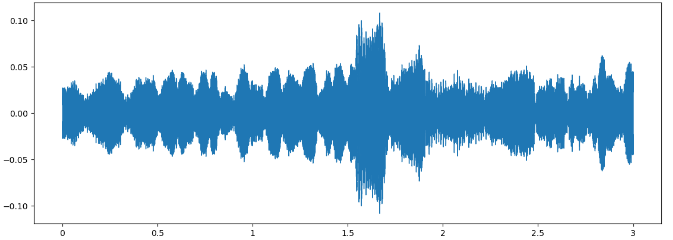
\includegraphics[width=\linewidth]{images/noise_augmentation_original_signal_intensity.png}
            \caption*{Original signal}
        \end{minipage}%
        \hfill%
        \begin{minipage}{0.49\textwidth}
            \centering
            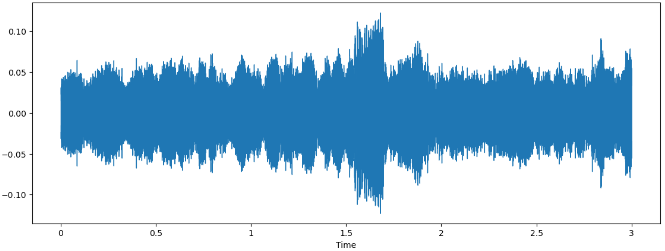
\includegraphics[width=\linewidth]{images/noise_augmentation_augmented_signal_01_intensity.png}
            \caption*{Original signal after noise injection}
        \end{minipage}
        
        \vspace{0.5cm}
        
        \begin{minipage}{0.49\textwidth}
            \centering
            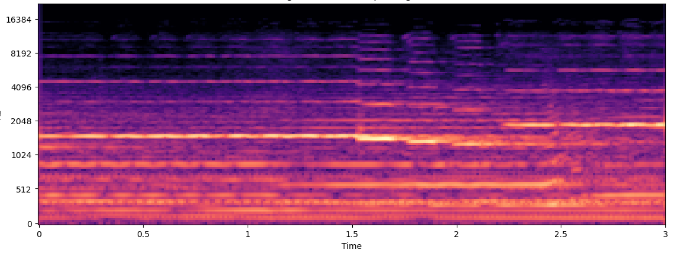
\includegraphics[width=\linewidth]{images/noise-injection-original-spectogram.png}
            \caption*{Mel-spectrogram of the original signal}
        \end{minipage}%
        \hfill%
        \begin{minipage}{0.49\textwidth}
            \centering
            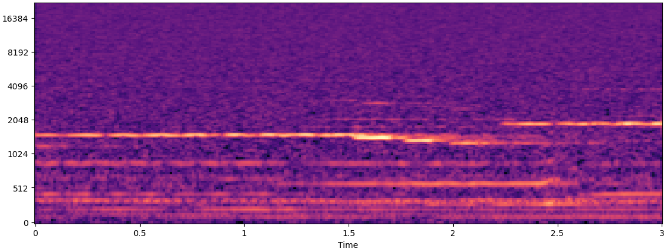
\includegraphics[width=\linewidth]{images/noise-injection-augmented-spectogram.png}
            \caption*{Mel-spectrogram of the signal after noise injection}
        \end{minipage}
                
        \centercaption{Example of the effect of noise injection, alpha=0.1}
        
        \label{fig:noise-injection}
        
    \end{figure}

Although the signal intensity plot does not show much difference between the original and augmented signal, the difference is obvious when looking at the mel-spectrogram representations of the signal. It also clarifies that using a too-large alpha value can significantly degrade the original signal, and depending on the representation used, potentially harm training. That is why we decided to choose a more conservative alpha value of 0.005 in our experiments.

\subsubsection{Pitch shift}

The second type of audio augmentation we used is pitch shift. This type of audio augmentation consists of shifting the pitch of the input signal by a random amount. In our experiments, we shifted the signal by a random number of semitones generated uniformly in range [-6,6]. It is important not to shift the pitch of the original signal too much, as it could end up outside the normal pitch range for that instrument. The effects of pitch shift augmentation can be seen in Figure~\ref{fig:pitch-shift}.

\begin{figure}[H]
        \centering
        
        \begin{minipage}{0.49\textwidth}
            \centering
            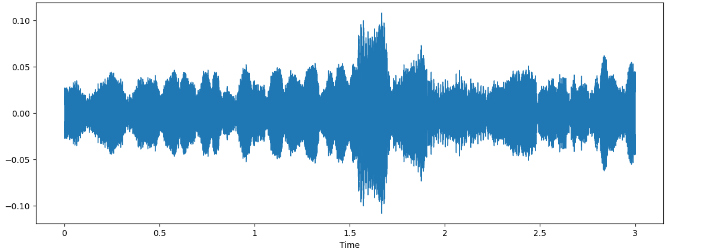
\includegraphics[width=\linewidth]{images/pitch-shift-original-audio-intensity.png}
            \caption*{Original signal}
        \end{minipage}%
        \hfill%
        \begin{minipage}{0.49\textwidth}
            \centering
            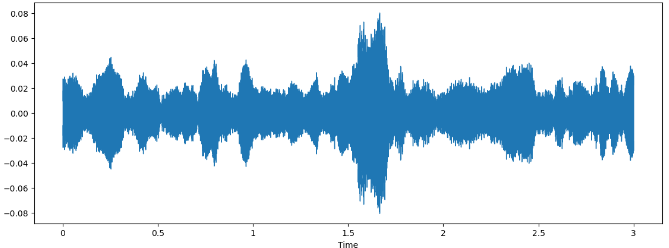
\includegraphics[width=\linewidth]{images/pitch-shift-augmented-audio-intensity.png}
            \caption*{Original signal after pitch shift}
        \end{minipage}
        
        \vspace{0.5cm}
        
        \begin{minipage}{0.49\textwidth}
            \centering
            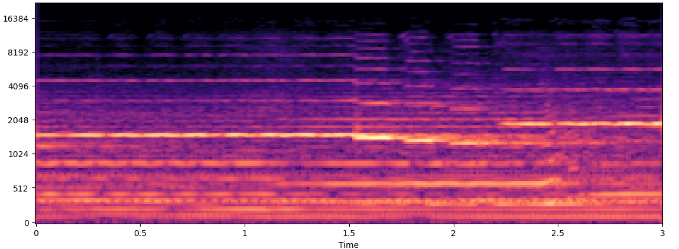
\includegraphics[width=\linewidth]{images/pitch-shift-original-audio-spectogram.png}
            \caption*{Mel-spectrogram of the original signal}
        \end{minipage}%
        \hfill%
        \begin{minipage}{0.49\textwidth}
            \centering
            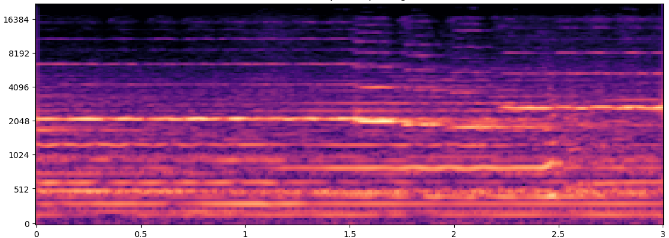
\includegraphics[width=\linewidth]{images/pitch-shift-augmented-audio-spectogram.png}
            \caption*{Mel-spectrogram of the signal after pitch shift}
        \end{minipage}
                
        \centercaption{Example of the effect of pitch shift up by 6 semitones}
        
        \label{fig:pitch-shift}
        
    \end{figure}

We can easily see the effects of the pitch shift in spectrograms in Figure~\ref{fig:pitch-shift}. We can see the yellow lines representing the presence of certain frequencies clearly shift up in the augmented spectrogram, compared to the original one.

\subsubsection{Time shift}

Finally, the third audio augmentation used is time shift. It consists of moving the entire signal by a certain amount forward or backward, so it starts and ends on a different part of the signal. The duration of the signal is not changed.  Let's say we time shift the original signal by 1 second forward. That would mean that the new signal now starts at the previous signal's one-second mark, and its last second is what used to be the first second of the original signal. The effect of this augmentation is best seen through visualizations in Figure~\ref{fig:time-shift}.

\begin{figure}[H]
        \centering
        
        \begin{minipage}{0.49\textwidth}
            \centering
            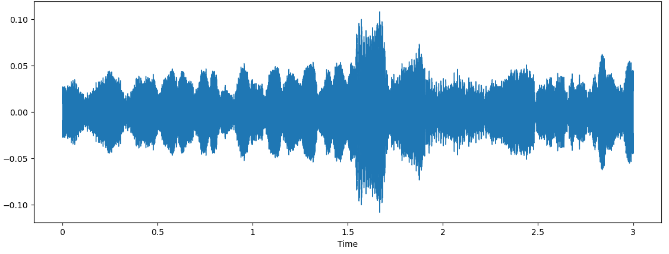
\includegraphics[width=\linewidth]{images/time-shift-original-intensity.png}
            \caption*{Original signal}
        \end{minipage}%
        \hfill%
        \begin{minipage}{0.49\textwidth}
            \centering
            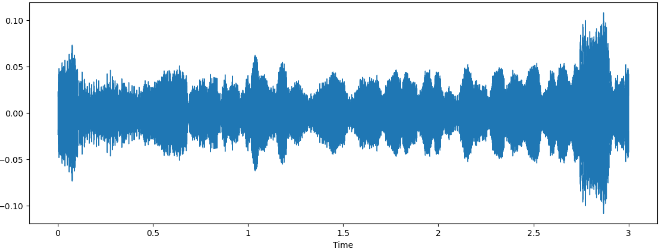
\includegraphics[width=\linewidth]{images/time-shift-augmented-intensity.png}
            \caption*{Original signal after time shift}
        \end{minipage}
        
        \vspace{0.5cm}
        
        \begin{minipage}{0.49\textwidth}
            \centering
            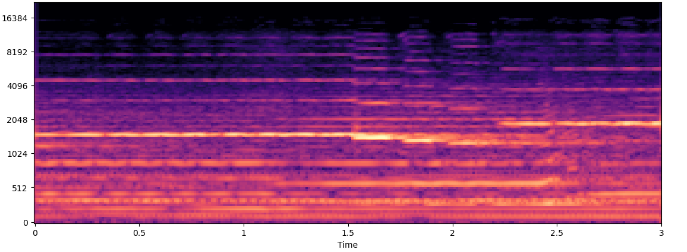
\includegraphics[width=\linewidth]{images/time-shift-original-spectogram.png}
            \caption*{Mel-spectrogram of the original signal}
        \end{minipage}%
        \hfill%
        \begin{minipage}{0.49\textwidth}
            \centering
            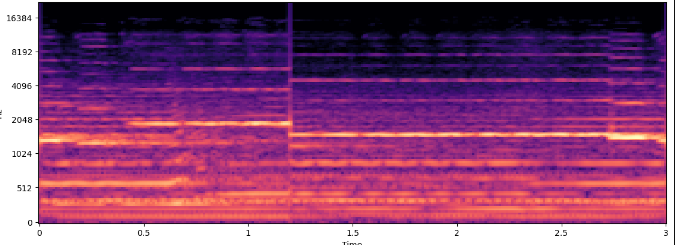
\includegraphics[width=\linewidth]{images/time-shift-augmented-spectogram.png}
            \caption*{Mel-spectrogram of the signal after time shift}
        \end{minipage}
                
        \centercaption{Example of the effect of time shift up 40\% of original length forwards}
        
        \label{fig:time-shift}
        
    \end{figure}

In our experiments, we performed time shifting by first randomly choosing a percentage in range [-0.4, 0.4], and then performing time shifting by shifting the original signal by the percentage of its original length forwards (if the chosen number was positive), or backward (if the chosen number was negative).

\subsection{Spectrogram augmentations}

The two spectrogram augmentations used in our experiments, time and frequency masking, were first introduced in \cite{specaugment}. The authors justify these augmentations by saying "These features (mel-spectrograms) should be robust to deformations in the time direction, partial loss of frequency information, and partial loss of small segments of speech." The essential idea of both techniques is the same - mask a part of the input spectrogram, forcing the model not to rely too much on any specific feature or part of the spectrogram, instead encouraging it to learn from more features, thus increasing its generalization.

\subsubsection{Frequency masking}

The first of these augmentations is frequency masking. As its name suggests, it consists of masking a block of consecutive mel frequency channels in the original mel spectrogram. The mask itself simply consists of the mean values of the entire spectrogram; this is important so as to not introduce any "foreign" information into the spectrogram. More formally, frequency masking is applied so that \textit{f} consecutive mel frequency channels $[f_0, f_0 + f)$ are masked, f being chosen uniformly in range [0, F], F being the frequency mask parameter, while $f_0$ is chosen in range $[0, v - f)$, where $v$ is the number of mel frequency channels. The effects of frequency masking can be seen in Figure~\ref{fig:frequency-masking}

\asideimages{7cm}{7cm}
	    {frequency-masking-original}
	    {Original spectrogram}
        {frequency-masking-augmented}
	    {Spectrogram after frequency masking}
	    {Example of the effect of frequency masking augmentation using two frequency masks}
	    {fig:frequency-masking}

During our experiments, we consistently created two frequency masks, with each mask occupying a portion (P) of the total frequencies. The value of P was uniformly selected from [0,10]. As two masks were used, the percentage of total frequencies masked in any given spectrogram could be at most 20\% and on average 10\%.

\subsubsection{Time masking}

The second type of spectrogram augmentation is time masking. It is, in essence, equivalent to frequency masking, except that it is done in the time domain of the spectrogram. Formally, time masking is applied so that $t$ consecutive time steps $[t_0, t_0 + t)$ are masked, where t is uniformly chosen in range $[0, T]$, $T$ being the time mask parameter, and $t_0$ chosen uniformly from $[0, \tau - t)$. $\tau$ is the number of time steps in the mel spectrogram. The effects of time masking can be seen in Figure~\ref{fig:time-masking}.

\asideimages{7cm}{7cm}
	    {frequency-masking-original}
	    {Original spectrogram}
        {time-masking-augmented}
	    {Spectrogram after time masking}
	    {Example of the effect of time masking augmentation using two time masks}
	    {fig:time-masking}

Same as in frequency masking, we always generated two time masks, each occupying P of the total time steps, P being chosen uniformly in range [0,10].

\subsubsection{Time + frequency masking}

Finally, we can see the combined effects of time and frequency masking in Figure~\ref{fig:time-frequency-masking}.

\asideimages{7cm}{7cm}
	    {frequency-masking-original}
	    {Original spectrogram}
        {time-frequency-masking-combined}
	    {Spectrogram after time and frequency masking}
	    {Example of the combined effect of time and frequency masking augmentation using two time and frequency masks}
	    {fig:time-frequency-masking}

\section{Dynamic sampling}
\label{sec:data-prep:dynamic-sampling}

The specific nature of the IRMAS dataset is, as has already been stated, that all the examples from the train set contain only a single label, while the examples in the test set may contain multiple labels per example. To mitigate this problem, instead of combining multiple train samples once and creating a single new set of training data with multiple labels,  we decided to implement a different approach we named \textbf{dynamic sampling}. In short, new training examples would be generated dynamically during training by randomly selecting and combining multiple examples with a single label into a new example containing multiple labels. In theory, this should greatly increase the variability of available data, as well as solve the issue of the training data having only a single label per example. In addition, it would save the space that static examples overlapping would occupy.

We implemented two types of dynamic sampling - true dynamic sampling, and base-sample-persistent dynamic sampling. We are going to shortly explain their differences and implementation, while the results we achieved will be presented in Chapter~\ref{ch:evaluation}.

\subsection{True dynamic sampling}

The "true" in the name of this type of dynamic sampling comes from the fact that every original example from which the final combined example consists is randomly selected at the moment the dynamic sampling function is called, thus meaning there is no dependency between two dynamic sampling calls or dependency between samples created in one epoch and another. The pseudocode for this sampling method is shown below:

\begin{algorithm}[H]
    \SetKwInOut{Input}{Input}
    \SetKwInOut{Output}{Output}

    \underline{function SampleTrueDynamic} $(minSampled, maxSampled, noClasses)$\;
    \Input{Minimum and maximum number of sampled examples, the total number of classes}
    \Output{sampled audio, list of labels in combined audio}
    noSamples = Random$(minSampled, maxSampled)$\;
    chosenLabels = RandomlySelectDistinctLabels$(noClasses, noSamples)$\;
    combinedAudio = None\;
    \For {label in chosenLabels}{
    \tcp{selects random audio out of all possible samples with the exception of samples with label \textit{label}} 
    audio = SelectRandomAudioExcludingLabel$(label)$ \;
    combinedAudio = CombineAudio$(combinedAudio, audio)$ \;
    }
    return combinedAudio, chosenLabels \;
    \caption{True dynamic sampling}
\end{algorithm}

Of course, this pseudocode only shows the sampling of a single sample; when training a model using dynamic sampling this method would be called many times, each time resulting in a new dynamically sampled example, made by combining multiple examples with single labels into a new example with multiple labels. Of course, a careful reader will have already asked themselves the following question: if the samples are now dynamically generated, how many samples should I generate, if I want to maximally utilize the data I already have available? And that is an excellent question, as due to the stochastic nature of the sampling process we have no guarantee of which original samples get sampled, possibly resulting in some examples being chosen for sampling many times, while other examples are not being chosen a single time. In order to solve this, you can use the following formula:

\DynamicSamplingNoSamples

The $N$ in the formula denotes the number of dynamic samples you have to generate to make sure that, on average, only $P$ \% of the total number of original examples do not get sampled within one epoch. $n$ is the total number of original examples, while minSampled and maxSampled represent the minimal and maximal number of original examples used when constructing a new, dynamically generated sample. The smaller the minSampled and maxSampled are, the larger $N$ has to be to maintain the same $P$. Table~\ref{tab:num-dynamic-samples} illustrates the effect  minSampled and maxSampled have on $N$, assuming $n$ is equal to the number of samples in the IRMAS training set, 6705, and $P$ value of 0.1\%, which we used in our experiments: 

\begin{table}[H]
\centering
\begin{tabular}{ccc}
\hline
minSampled & maxSampled & N     \\ \hline
1          & 2          & 30875 \\
1          & 3          & 23156 \\
1          & 4          & 18525 \\
1          & 5          & 15437
\end{tabular}
\caption{Effect of the minimal and maximal number of examples sampled using dynamic sampling on N}
\label{tab:num-dynamic-samples}
\end{table}

We can see that, if we want to dynamically sample and merge only two of the original samples at a time, we need to generate more than 30,000 dynamic samples, or almost 6x the size of the original dataset. On the other hand, if we dynamically sample and merge up to five original samples at a time, then a number of 15,437 suffices, which is rather more manageable. That is why in our experiments we usually used 4 or 5 for the value of maxSampled, while, of course, keeping minSampled at 1, as to sample certain examples as is.

One important advantage of this sampling method, in contrast, to sequentially iterating over examples in the training dataset, is that it follows a two-step process. Firstly, we uniformly choose the labels of the examples we intend to merge. Secondly, we uniformly select an example from all the available examples with each chosen label. Consequently, this approach ensures that, on average, every label (class) is sampled an equal percentage of times, thereby naturally balancing the distribution of classes within the dataset and increasing the macro performance metrics.


\subsection{Base-sample-persistent dynamic sampling}

The second type of dynamic sampling we considered is base-sample-persistent dynamic sampling. It is similar to true dynamic sampling, except for the following difference: the sampling method receives an initial sample (audio) and then builds upon it by selecting additional samples and merging them with the base sample. In practice, you would iterate over every sample \textbf{in the original training set}, assigning that sample the role of the base-sample, and, using base-sample-persistent dynamic sampling, merge it with $N$ other randomly chosen samples. This way, the base samples are consistent through every epoch; the only difference is the samples they are merged with.

The main idea behind this approach is to deal with very high variability in data which occurs when using true dynamic sampling, possibly leading to unstable training and the inability of the network to learn the distribution of samples. Furthermore, this sampling method \textbf{does not require} a large number of samples to work as does true dynamic sampling; as the base sample remains the same in every epoch, we have a guarantee that every sample from the original training data is going to get chosen at least once per epoch and usually more. The pseudocode of the algorithm is shown below: 

\begin{algorithm}[H]
    \SetKwInOut{Input}{Input}
    \SetKwInOut{Output}{Output}

    \underline{function SampleBasePersistent} $(baseSample, minSampled, maxSampled, noClasses)$\;
    \Input{Base sample, minimum and maximum number of sampled examples, the total number of classes}
    \Output{sampled audio, list of labels in combined audio}
    noSamples = Random$(minSampled, maxSampled)$\;
    chosenLabels = RandomlySelectDistinctLabels$(noClasses, noSamples)$\;
    \For {label in chosenLabels}{
    \tcp{selects random audio out of all possible samples with the exception of samples with label \textit{label}} 
    audio = SelectRandomAudioExcludingLabel$(label)$ \;
    baseSample = CombineAudio$(combinedAudio, baseSample)$ \;
    }
    return baseSample, chosenLabels \;
    \caption{Base-sample-persistent dynamic sampling}
\end{algorithm}

\section{Data splits}

We split the available datasets into training, validation, and testing datasets. The same splits were then used for training, validation, and testing of every model, to enable better comparison between models.

\subsection{IRMAS}
For IRMAS, we used the original train set in unchanged form as our train set. This dataset consisted only of examples with a single label. To generate validation and test sets, we split the provided evaluation dataset, which consisted of examples with one and more labels, into validation and test sets using a ratio of 70-30. After the split, the validation dataset consisted of 862 examples and the test dataset of 2010 examples. The training dataset remained unchanged at 6704 examples. 

\subsection{Audioset}

We collected a total number of 20,884 samples from the original Audioset dataset. Those samples were then split into training, validation, and testing datasets using a ratio of 70-10-20, resulting in the training set of size 14,618 examples, a validation set of size 2088, and a testing set of size 4176.
        \newchapter{Modeling}{ch:modeling}
\label{ch:modeling}

An overview of the models we've used in given in Table~\ref{tab:models-overview}. We've trained some of the models from scratch and used some pre-trained ones as well. The models trained from scratch were not expected to perform better than the pre-trained once. Instead, they were used to show the effectiveness of specific features and approaches, e.g. 1d vs 2d convolution. 

\EQbce

The loss function, which was the same for all the models, was the binary cross-entropy (BCE) loss, whose loss formulation is given in Eq.~\ref{eq:bce}. $N$ denotes the batch size. Mean reduction was applied over the batch size. We used BCE loss instead of the CE loss because we have a multi-label problem. That means that each example can be labeled with multiple labels. CE loss is suitable for multi-class problems, where we have multiple class, but only one label can be positive.

\begin{table}[H]
\centering
\begin{tabular}{l c c r}
Model & Architecture & Pre-trained & Num. params.   \\ \hline
Raw audio 1-D CNN & CNN & No & 180 K                      \\
MFCC 2-D CNN & CNN & No & 879 K                      \\
Audio features 1-D CNN & CNN & No & 114 K                      \\
ResNet50 & CNN & Yes & 23.5 M                     \\
AST & Transformer & Yes & 86.2 M                                             
\end{tabular}
\caption{Overview of the models used}
\label{tab:models-overview}
\end{table}

Throughout all the experiments we used the Adam optimizer \cite{kingma2014adam}. It is the state-of-the-art (SOTA) approach, so we choose it over the standard stochastic gradient descent (SGD). As for the scheduler, we did some early experiments with the scheduler which reduces the learning rate on plateau, e.g. when loss (or potentially other specified metric) has not decreased for $k$ epochs. The problem was that we had to define the hyperparameter $k$, which again requires some trial and error. Instead, we switched over to the polynomial decay scheduler. For the polynomial decay scheduler, we had to define the starting and desired ending learning rate, along with the polynomial factor. The factor of 1 corresponds to linear decay. We choose the factor of $0.7$. Furthermore, we decided to use the learning rate warmup of $0.05$. Warmup is the training period in which the learning rate linearly increases from effectively 0 to the defined starting learning rate. It us useful so that the initial training steps do not \textit{overshoot} with gradient updates. Instead, small steps towards the minimum are performed at the beginning, and larger steps after the initial movement towards the minimum had already started rolling. In Figure~\ref{fig:lr}, we show the behaviour of our learning rate throughout the training. As for the regularization, we used L2 regularization, which is implemented as weight decay in the PyTorch's version of the Adam optimizer\footnoteurlwithoutheader{https://pytorch.org/docs/stable/generated/torch.optim.Adam.html}{https://pytorch.org/docs/stable/generated/torch.optim.Adam.html}. We used different weight decay values throughout the experiments, which will be later discussed in Section~\ref{sec:eval:ast}.

\imagefigurecaption[0.5]{lr-polynomial-example}
	        {Learning rate behaviour throughout the training.}
                {fig:lr}

\section{Raw audio 1-D CNN}
\label{sec:raw-audio-1d-cnn}
Among the simplest convolutional approaches is the 1-dimensional convolution on the raw audio waveform. The input was a 1 second window with sample rate $44.1$ kHz, resulting in the input shape of (batch size, 1, 44100). Due to the disproportional sizes, the architecture cannot be shown in an image. Instead, we show it in Table~\ref{tab:architecture-1d-cnn-raw-audio}. The idea was to use the first kernel size corresponding to 10 ms of the audio as we believed that was a reasonable time frame to be able to extract some useful information. We omit mentioning ReLU and BatchNorm1d between each Conv1d and MaxPool1d layer. We also omit mentioning ReLU and dropout between the linear layers. No pre-trained layers were used. The hyperparameters are the same as in Table~\ref{tab:2d-conv-mfcc-hyperparam}.

\begin{table}[H]
\small
\centering
\begin{tabular}{l l c}
Layer                    & Shape in                   & Kernel \\ \hline
Conv1d                   & (B, 1, 44100)            & (1, 440), stride = 2          \\
MaxPool1d ($4 \times 4$) & (B, 32, 21831)            & -          \\
Conv1d                   & (B, 32, 5457)            & (1, 6), stride = 1          \\
MaxPool1d ($4 \times 4$) & (B, 32, 5452)            & -          \\
Conv1d                   & (B, 32, 1363)            & (1, 3), stride = 1          \\
MaxPool1d ($4 \times 4$) & (B, 64, 1361)            & -          \\
Conv1d                   & (B, 64, 340)            & (1, 3), stride = 1          \\
MaxPool1d ($4 \times 4$) & (B, 64, 338)            & -          \\
Conv1d                   & (B, 64, 84)            & (1, 3), stride = 1          \\
MaxPool1d ($4 \times 4$) & (B, 128, 82)            & -          \\
Conv1d                   & (B, 128, 20)            & (1, 3), stride = 1          \\
MaxPool1d ($4 \times 4$) & (B, 256, 18)            & -          \\
AvgPool1d                & (B, 256, 4)             & -          \\
flatten                  & (B, 256, 1)              & - \\
linear\_1                & (B, 256)                 & -          \\
linear\_2                & (B, 64)                 & -          \\
output (no weights)      & (B, 11)                  & - 
\end{tabular}
\caption{Architecture of a 1-D CNN on raw audio}
\label{tab:architecture-1d-cnn-raw-audio}
\end{table}

\section{MFCC 2-D CNN}
\label{sec:mfcc-2d-cnn}
MFCC is a 2-dimensional feature, which makes it suitable for 2-d convolutional layers. We decided on extracting 40 cepstral coefficients in order to make more room for our convolutions and in belief that it would potentially bring more valuable information, as explained in Section~\ref{sec:data-prep:mfcc}. Due to lack of time, we did not experiment with 13 coefficients, although it would be an interesting comparison. We leave that for future work. We additionally resize the width of the image to 256 in order to make it universal and capable of handling different input sizes. The only input length we have tried was the 1 second window at the sample rate of $44.1$ kHz. The architecture is shown in Figure~\ref{fig:2d-cnn-mfcc} and hyperparameters in Table~\ref{tab:2d-conv-mfcc-hyperparam}. No pre-trained weights were used. The input had one channel and we apply four convolutional blocks which contain (Conv2d, ReLU, BatchNorm2d, MaxPool2d). Afterwards, average 2-dimensional pooling is applied, tensor is flattened and fed into two linear layers with a 20 \% dropout and ReLU non-linearity in between. 

\imagefigurecaption[1.0]{2d-cnn-mfcc}
	        {2-dimensional CNN architecture on MFCC features}
                {fig:2d-cnn-mfcc}

\begin{table}[H]
\centering
\begin{tabular}{l r}
Hyperparameter           & Value   \\ \hline
Initial learning rate    & 1e-3                        \\
Final learning rate      & 1e-5                        \\
Learning rate scheduler  & Polynomial decay, power=0.7, warmup=0.05 \\
Number of epochs         & 35                          \\
Batch size               & 16                          \\
L2-regularization factor & 5e-4                       
\end{tabular}
\caption{Hyperparameters of our 1-D raw audio, 2-D MFCC, and 1-D audio features CNN models}
\label{tab:2d-conv-mfcc-hyperparam}
\end{table}

%\begin{figure}[thb]
%    \centering
%    \includesvg[width=0.8\linewidth]{images/2d-cnn-mfcc.svg}
%    \caption{2-dimensional CNN architecture on MFCC features}
%    \label{fig:2d-cnn-mfcc}
%\end{figure}

\section{Audio features 1-D CNN}
\label{sec:audio-features-1d-cnn}
For the convolutional model on the extracted audio features, we take a very experimental approach. After discussing the statistical significance of the features in Section~\ref{sec:statistical-testing}, we omit tonnetz feature due to its insignificance. Additionally, we omit spectrogram, as it was covered by other, more powerful models (see Sections~\ref{sec:spectrogram-resnet},~\ref{sec:ast}). After including the features, we are left with 40 of them. Now, since most of these features do not interact, it would be incorrect to just stack the features vertically. Instead, we decided to feed each feature as a separate channel into the 1-dimensional convolution. Feeding each feature in a separate channel allows the model to learn individual patterns and correlations for each feature. However, it does not allow feature interactions. This is something we do want to avoid between, for example, zero-crossing rate and chroma features. However, this is something we would like to have between chroma features themselves. So, this approach was done out of curiosity to see if it would be more beneficial for the model to avoid learning unnecessary correlations between uncorrelated features more than it would be learning the correlations between both correlated and uncorrelated features. Unfortunately, due to the lack of time, we did not have time to test the 2-dimensional convolution on all the audio features. Thus, we leave that for future work. However, we can compare the results with the previously discussed 2-d convolution of MFCC features, which we will do in Chapter~\ref{ch:evaluation}.

\imagefigurecaption[1.0]{1d-cnn-audio-features}
	        {1-dimensional CNN architecture on extracted audio features}
                {fig:1d-cnn-audio-features}

The architecture of the model is shown in Figure~\ref{fig:1d-cnn-audio-features} and the hyperparameters in Table~\ref{tab:2d-conv-mfcc-hyperparam}. Again, the only window we experimented with was or size 1 second. Consequently, with n\_fft, hop\_length, frame\_length, and sample\_rate equal to 2048, 512, 2048, and $44100$ respectively, we obtain an input of shape $H \times W$. Here, $H$ is the number of features (40) and $W$ is the example length derived when using the mentioned parameter values (87). The features are, however, fed into separate channels. Again, four (Conv1d, ReLU, BatchNorm1d, MaxPool1d) blocks are used with the average 1-dimensional pooling applied afterwards. Finally, the tensor is flattened and fed into two linear layers with a 20 \% dropout and ReLU non-linearity in between. Logits are returned from the model's forward pass. 

\section{Spectrogram -- ResNet50}
\label{sec:spectrogram-resnet}

Perhaps one of the most famous and widely used neural network architectures is ResNet, first introduced in \cite{resnet}. In an attempt to mitigate the problems of vanishing and exploding gradients, which tend to appear more and more often as the depth of the network increases, authors of ResNet introduce a concept of a \textbf{residual unit}. Residual units enable the network to

\begin{enumerate}[label=(\alph*)]
\item utilize skip connections, allowing the input data to skip a couple of layers, which in turn helps stop the exploding/vanishing gradient problems and reduce overfitting, by acting as a sort of dropout
\item learn \textbf{residual mappings}, which allow the layer of a network to form an identity function that maps to an activation earlier in the network when a specific layer's activation converges to zero in the current layer. This also helps with the degradation of performance in the deeper layers, as the network can simply "revert" to an earlier layer's output
\end{enumerate}

\imagefigurecaption[0.8]{resnet-block}
	        {Visualisation of a residual unit, one of the key building blocks of residual networks \cite{resnet}}
                {fig:resnet-block}

Due to its unique architecture and the use of residual blocks, residual networks support a large number of layers - it is not uncommon for a residual network to have 50, 101, or even 152 layers. The number of layers used in residual networks is usually denoted by a number next to their name; for example, a residual network with 101 layers would be denoted as ResNet-101. 

Of course, training such a deep network from scratch would require a large amount of data in order for the network to work well. So, a usual approach is to pre-train the network on a general image-related task (if the network is used for computer vision, of course, as ours was), such as classification on the large ImageNet dataset. The weights from that pre-trained model are then used as a starting point, in addition to replacing the final fully-connected layer with a new one, depending on the specific nature of the problem. This approach is known as \textbf{transfer learning} and is widely used.

We choose ResNet as the main convolutional network for spectrograms as it has proven itself to be a powerful and versatile network well suited to a wide array of applications. Furthermore, it has a large capacity, allowing it to better learn the distribution of our data, especially when using augmentation methods  such as dynamic sampling, which add a high degree of variability.

Our version of the ResNet architecture was ResNet-50, pre-trained on ImageNet-1K. We replace the final fully-connected layer with our own and add a dropout layer with p=0.2 between the FC layer and the output of the base ResNet-50 model. Hyperparameters used to train all the ResNet-50 models were, unless explicitly stated otherwise, the ones in Table~\ref{tab:resnet-hyperparams}.

\begin{table}[H]
\centering
\begin{tabular}{l r}
Hyperparameter           & Value   \\ \hline
Initial learning rate    & 2e-4                        \\
Final learning rate      & 1e-6                        \\
Learning rate scheduler  & Polynomial decay, factor=0.7, warmup=0.05 \\
Number of epochs         & 35                          \\
Batch size               & 16                          \\
L2-regularization factor & 1e-5                       
\end{tabular}
\caption{Standard hyperparameters of our ResNet-50 model}
\label{tab:resnet-hyperparams}
\end{table}



\section{Audio Spectrogram Transformer}
\label{sec:ast}
The only model with no convolutional layers is the Audio Spectrogram Transformer (AST) \cite{gong2021ast}. There are multiple layers to decouple in the definition and background of AST. First, the backbone of the whole architecture is the Transformer \cite{vaswani2017attention}. It was originally proposed for the Natural Language Processing (NLP) problems. However, due to its incredible parallelism, model depth, and attention mechanism, it had achieved great success in models such as BERT \cite{devlin2018bert}, GPT-3 \cite{brown2020language}, XLNet \cite{yang2019xlnet}, T5 \cite{raffel2020exploring} etc. Consequently, it was adjusted to be able to handle vision inputs in the similar way it handles text -- in parallel. That is how the Vision Transformer (ViT) \cite{kolesnikov2021image} was born. Finally, since spectrograms are the most often feature used in audio classifications, ViT was further trained on the complete Audioset dataset \cite{audioset2017}(Section \ref{sec:audioset}). That is the simplified story of how AST came to life. In the next few paragraphs, we will go over the important details of the (Vision) Transformer.

\asideimagesnocite{4cm}{9.5cm}
	    {transformer-encoder}
	    {Transformer encoder \cite{kolesnikov2021image}}
	    {ast-architecture}
	    {AST architecture \cite{gong2021ast}}
	    {Audio Spectrogram Transformer \cite{kolesnikov2021image, gong2021ast}}
     %\footnotewithoutheader{Images taken from \cite{kolesnikov2021image} and \cite{gong2021ast} respectively.}
	    {fig:ast-architecture}

The originally proposed Transformer is made of the encoder and decoder part. The encoder's task is to extract useful information from the input text (image), while the decoder's task is generating text (image) from the input and previously extracted information. As we require only the discriminative model, we discard any discussion on the decoder and focus solely on the encoder. It is shown in Figure~\ref{fig:ast-architecture}(a). The input, which we will explain later, is passed onto the sequence of $L$ layers, whose architectures are shown in grey. In out case, $L$ was equal to 12. After normalization all the inputs (text tokens or image patches) are in parallel passed onto the Multi-Head Attention (MHA) sub-layer. \textit{Multi-head} indicates multiple attention heads (layers), but let's focus on a single one for now. First, each input token (patch), is used to create a Query (Q) vector, a Key (K) vector, and a Value (V) vector. These vectors are created by multiplying the embedding by Query, Key, and Value matrices respectively. These matrices are trained end-to-end during the process. The resulting Q, K and V vectors are passed onto the scaled dot-product attention (Figure~\ref{fig:attention}(a)) to calculate how much does each token (patch) \textit{attend} to the others, i.e. how connected or important they are to each other in some abstract way which the model learns itself. It is important to mention that this is the simplified explanation, since the vectors are passed as part of the matrices in the original implementation. After calculating the scaled dot-product attention of the matrices for each head, the outputs are concatenated and multiplied with yet another weight matrix (Figure~\ref{fig:attention}(b)). What follows are the residual connection and another layer normalization. Transformer architecture is well equipped with residual connections due to its depth, which allows the gradients to be passed all the way to the first layers during gradient backpropagation. To continue, the output is passed through two feed-forward layers, another residual connection is applied and the final outputs are passed onto the next layer for the same treatment. Each layer receives the output of the previous layer, with the exception of the first layer, which receives the input, which we will now discuss. 

\asideimagesnocite{2.5cm}{4.6cm}
	    {scaled-dot-product-attention}
	    {Scaled dot-product attention \cite{kolesnikov2021image}}
	    {mha}
	    {Multi-Head Attention \cite{gong2021ast}}
	    {Transformer's attention mechanism}
     %\footnotewithoutheader{Images taken from \cite{kolesnikov2021image} and \cite{gong2021ast} respectively.}
	    {fig:attention}

The biggest contribution of ViT is, in our opinion, the way they adjust the image input to be appropriate for the Transformer architecture, just as text tokens are. 
As discussed in \cite{kolesnikov2021image}, the standard Transformer receives as input a 1D sequence of token embeddings. To handle images, they reshape the image $\mathbf{x} \in \mathbb{R}^{H \times W \times C}$ into a sequence of flattened 2D patches $\mathbf{x}_p \in \mathbb{R}^{N \times (P^2 \cdot C)}$, where ($H$, $W$) is the resolution of the original image, $C$ is the number of channels, ($P$, $P$) is the resolution of each image patch, and $N = HW / P^2$ is the resulting number of patches, which also serves as the effective input sequence length for the Transformer. The Transformer uses constant latent vector size $D$ through all of its layers. Thus they flatten the patches and map to $D$ dimensions with a trainable linear projection (see Figure~\ref{fig:ast-architecture}). The output of this projection is referred to as patch embeddings. For the base-sized models (and the model we had used) the size of the patch embedding is 768.

There is a slight difference in creating the input for AST. According to \cite{gong2021ast}, the input audio waveform of $t$
seconds is first converted into a sequence of 128-dimensional log
Mel filterbank (fbank) features are computed with a 25ms Hamming window every 10ms. This results in a $128 \times 100t$ spectrogram as input to the AST. The spectrogram is then split into a sequence of $N$ $16 \times 16$ patches with an overlap of 6 in both time
and frequency dimension, where $N = 12 \left\lceil (100t - 16)/10 \right\rceil$ is
the number of patches and the effective input sequence length for the Transformer. The patch is again flattened and linearly projected to a patch embedding of size 768. In order to fix these previously discussed numbers, AST requires users to use the sample rate of $16$ kHz. Thus, we down-sampled our audio files from $44.1$ kHz to $16$ kHz.

Since the patch embedding is not in temporal order and the architecture itself has no mechanism of capturing the input order, they add a trainable 768-dimensional positional embedding in order to capture the information about the spatial structure of spectrograms. Positional embeddings are denoted with a blue color and letter \texttt{P} in Figure~\ref{fig:ast-architecture}. The most important embedding, however, is the \texttt{[CLS]} embedding which is appended at the beginning of the sequence and passed later onto the single linear layer to obtain the output. As its name suggests, this embedding is used for classification purposes. The Transformer Encoder's output of the \texttt{[CLS]} embedding serves as the audio spectrogram representation \cite{gong2021ast}. In our use case, the 768-dimensional \texttt{[CLS]} embedding was linearly projected by a $768 \times 11$ (num\_classes) matrix to obtain \texttt{logit} outputs for each class. We used Huggingface\footnoteurlwithoutheader{https://huggingface.co/docs/transformers/main/en/model\_doc/audio-spectrogram-transformer}{https://huggingface.co/docs/transformers/main/en/model\_doc/audio-spectrogram-transformer} implementation of an AST.

According to Huggingface's specification, a maximum spectrogram length that can be fed into AST is 1024. With the sample rate of $16$ kHz, this is equal to about 10 seconds of audio. Longer files get truncated, while the shorter ones are padded. We tried two approaches. First, we used AST as is, with pre-trained position embeddings and 10 second audio files. This has downsides of (a) longer training time due to longer (default) input and (b) much of padding and truncating is applied. Second, we tried fixing the input length to 1 second by using multiple windows on a single file. This has a downside of training completely new positional embeddings, due to the new width of input spectrograms. In total $1214 \times 768 = 932,352$ positional embeddings were discarded and $110 \times 768 = 84,480$ new ones were randomly (with normal distribution) initialized and trained. Just as a reference, the discarded positional embeddings contain more parameters than any of the raw audio 1-D CNN, MFCC 2-D CNN, and audio features 1-D CNN models! However, the benefit of such approach is a much faster training time and no padding/truncating. Hyperparameters used to train all the AST models were, unless explicitly stated otherwise, the ones in Table~\ref{tab:ast-hyperparams}. We increased number of gradient accumulation steps according to the maximum batch size that could fit into the GPU memory. For the 10 second, the maximum batch size was 1, so we increase gradient accumulation steps to 16. Separate optimizer and schedulers were used for the (a) classifier and (b) all the other parameters. The reason for this is that the classifier is not pre-trained. Instead, it is randomly initialized using the normal distribution. Thus, we do not want to preserve any knowledge from before by using a small learning rate, like we do for the rest of the AST parameters. 

\begin{table}[H]
\centering
\begin{tabular}{l r}
Hyperparameter           & Value   \\ \hline
Initial learning rate (base)    & 2e-5                        \\
Final learning rate (base)     & 2e-6                        \\
Initial learning rate (classifier)    & 1e-3                        \\
Final learning rate (classifier)     & 1e-4                        \\
Learning rate scheduler  & Polynomial decay, factor=0.7, warmup=0.05 \\
Number of epochs         & 35                          \\
Batch size               & 16                          \\
L2-regularization factor (base) & 1e-4                  \\
L2-regularization factor (classifier) & 1e-3                  
\end{tabular}
\caption{Standard hyperparameters of our AST model}
\label{tab:ast-hyperparams}
\end{table}

\section{Window size}
\label{sec:window-size}
Audio files are, as we already mentioned multiple times, unique in many ways when compared to other forms of data. One of the main ways they are unique is their variable size, which can often present a problem for neural networks. A good example is the IRMAS dataset -- all the examples from the training set are 3s in length, while the data used for testing can vary anywhere between 5 and 20s. So, it is important that our model is good at working with files of different lengths, often different from what the model had been trained on. A good way of solving this is by splitting the full-length audio into windows of the same size, analyzing each section and predicting instruments it contains, and then aggregating outputs of all the windows into a single output, which is then equal to the prediction for the entire audio clip. By doing this, our network can be efficiently trained to work with fixed-size inputs (for example, 1s), and can later work with inputs of any size, as all inputs are split into windows equal in length to the window the network had been trained on. This approach is inspired by the work of \cite{hanetal_2016}, who also empirically prove that neural networks trained on the task of predominant instrument recognition are more efficient when trained and evaluated using shorter window sizes (1s) when compared to larger window sizes (3s). They claim that using a shorter window size helps obtain local instrument information. We confirm this finding in our own results, as shown later in Section~\ref{sec:eval:window-sizes}.

IRMAS dataset is especially suited to this approach, as it guarantees that the instrument audio clip is labeled with is playing the entire length of the clip. This means that when training a model, original examples of lengths N can be split into M windows, each of lengths N/M, and each carrying the label of the original clip. In addition to allowing the network to train on shorter clips, this also acts as an augmentation strategy, increasing the number of examples used during training.

\section{Aggregation functions}
\label{sec:aggregation-functions}

The question remains, once a prediction is made for every window of the original audio clip, how to aggregate all the predictions into a final prediction?

The authors of \cite{hanetal_2016} provide two aggregation strategies. The first, one, they call S1, is simply taking the average of the sigmoid outputs \textbf{class-wise}, and then thresholding them without normalization. The goal of this method is to "capture the existence of each instrument with its mean probability such that it might return the result without any detected instrument" \cite{hanetal_2016}. The second strategy, called S2, is done as follows: all sigmoid outputs are summed class-wise over all the window-based predictions for the audio clip. The values are then normalized by dividing with the maximum value amongst classes, so the normalized values fall into the [0,1] range. The normalized values are then thresholded, and all the classes with values over the threshold $T$, are taken as positive. The logic behind this method is based on the assumption that humans perceive the "predominant" instrument in a scaled sense; the strongest instrument is always detected, and the detection of the other instruments is judged relative to their strength compared to the most dominant instrument. In our case of predominant instrument classification, all instruments with predicted values above the threshold (after aggregation) are considered predominant. The authors found that, in general, the S2 aggregation strategy with a threshold value of 0.5 provides the best results, so this was the strategy we also used in our experiments. 


        \newchapter{Evaluation}{ch:evaluation}

In this section, we will go over evaluating our experiments. After building the models and running them, it is important to evaluate and compare them properly. Additionally, we will describe some additional steps we took in order to best utilize our models and their outputs to achieve better results.

\section{Metrics}
\label{sec:metrics}
To start with, we define the metrics used for the evaluation of our models. As stated by the competition organizer, \textbf{hamming score} is used for the final evaluation, so we include it in our evaluation as well. For the multi-label classification problem, Hamming score, macro accuracy, and micro accuracy have the same metric values. However, Hamming score does not account for label imbalance. As we believe that performing well on all of the labels, not just the high-resource ones, is very important, we include \textbf{macro F1-score} in our evaluation. Additionally, when we want to discuss the precision and recall of some of our models separately, we discuss the \textbf{macro precision} and \textbf{macro recall}. Additionally, we include \textbf{exact match accuracy}, which accounts for the number of examples whose predictions were exactly matched divided by the total number of examples. 

When choosing the best model, we look into the performance on the validation set. Since we kept the maximum of one checkpoint during the entire training, we needed to define the validation metric which will be used for deciding whether or not a checkpoint should be saved. We choose the validation loss as the metric. More specifically, we chose the validation loss calculated after performing the S2 aggregation over the validation examples. The reason behind this decision is that the same aggregation technique will be used for testing the model, so we wanted to actually save the model that is later most likely to perform the best on test data. We did not choose other metrics, such as hamming score and macro F1-score, because they do not give any insight into how confident is the model in its predictions. A checkpoint with the lowest validation loss should be the most general and should not suffer from overfitting. 

\section{Window sizes}
\label{sec:eval:window-sizes}
We start by discussing the effect of different window sizes (Section~\ref{sec:window-size}) during training and evaluation. We conduct this experiment using the ResNet model. Three different models were trained using respective window sizes of 1, 2, and 3 seconds on training, validation, and test data. The S2 aggregation function was used during evaluation, as introduced in Section~\ref{sec:aggregation-functions}. The results are shown in Figure~\ref{fig:resnet-window-sizes}. We observe that using the window size of 1 second performs slightly better than the window size of 2 or 3 seconds. Thus, we use the window size of 1 second and the aggregation function S2 throughout most of our experiments conducted on the IRMAS dataset later.
\imagefigurecaption[0.9]{resnet-window-sizes-comparison}
	        {ResNet performance on IRMAS test set using different window sizes}
                {fig:resnet-window-sizes}

\section{Non-pretrained CNN models}
\label{sec:eval:cnn-models}
After finding the optimal window size for the IRMAS dataset, we evaluate our non-pretrained CNN models. All the models were trained exclusively on IRMAS, using the previously found optimal window size of 1s. The performance comparison is shown in Figure~\ref{fig:cnn-performance}(a). The window size was 1 and the aggregation function was S2. To start with, the performance is significantly worse than ResNet. That is expected since ResNet is a pre-trained model with $27 \times$, $131 \times$, and $206 \times$ more parameters than MFCC 2-D CNN, raw audio 1-D CNN, and audio features 1-D CNN respectively. Next, comparing the performance of the non-pretrained CNN models themselves, it varies by different degrees for different metrics. Although the hamming score is very similar for all three models, with 1-D CNN audio features model being slightly worse, exact match accuracy performance and especially macro F1 performances vary. After noticing such a discrepancy, we additionally decided to plot the macro precision and macro recall of the two models on Figure~\ref{fig:cnn-performance}(b). The plots show that the CNN raw audio model has a much higher recall than the CNN audio features model, with their precision values almost the same. This suggests that performing a convolution directly on the raw audio allows us to catch more of the total positive labels. However, when claiming that some label in the example is positive, these two models have a similar hit rate. The fact that this happens implies that the CNN model on raw audio causes more positive labels in total compared to the CNN model on audio features, with a similar hit rate when claiming that some instrument (or voice) is present in the example. This suggests the convolution on the raw audio managed to learn the data better than the convolution on the audio features passed into separate channels.

\asideimages{14cm}{14cm}
	    {cnn-performance}
	    {Hamming score, exact match accuracy, and macro F1 score comparison on IRMAS test set.}
	    {cnn-precision-recall}
	    {Macro precision and recall comparison of 1-D CNN audio features and 1-D CNN raw audio models.}
	    {Performance comparison of the non-pretrained CNN models using the window size 1s}
	    {fig:cnn-performance}

Regarding the better exact match accuracy performance of the audio features CNN model, it is probably due to the model learning some spurious patterns in the data. This possibly led to the model performing well on specific audio instances (e.g. predicting all the labels correctly), but being unable to generalize well. This shows the importance of using and inspecting different performance metrics before making any conclusions. 


\section{Dynamic Sampling}
\label{sec:eval:dynamic-sampling}
Two dynamic sampling methods were introduced in Section~\ref{sec:data-prep:dynamic-sampling}. For the sake of comparison of the dynamic sampling methods (with the non-dynamic sampling model), we go back to the ResNet. The performance comparison is shown in Figure~\ref{fig:resnet-dynamic}(a). As previously mentioned, we sample and overlap anywhere from 1 to 5 examples at a time. We have experimented with sampling the maximum of 4 and the maximum of 5 examples as the time, which is denoted as -4 and -5 on the graph labels. \textit{true-dynamic-5} denotes that 5 samples were dynamically sampled and overlapped. \textit{base-sample-persistent-dynamic-5} indicates that, including the current sample, a maximum of 5 samples were included, i.e. maximum of 4 additional. We also experiment with window sizes of 1 and 3 seconds, which is denoted on the graph as \textit{window-1} and \textit{window-3}. Two different dynamic sampling techniques are denoted as \textit{true-dynamic} and \textit{base-sample-persistent-dynamic}. None of the 4 examined methods achieves significantly better results than the others. Since dynamic sampling generally causes more positive labels within the sample, we were interested in how that affects precision and recall. Figure~\ref{fig:resnet-dynamic}(b) shows that the model trained using dynamic sampling has higher recall and lower precision. This intuitively makes sense. Dynamic sampling caused the model to see more positive labels within the samples during training, which consequently makes it label more of them as positive during evaluation. This increases the recall, but decreases the precision, leaving the F1-score roughly the same. This is useful if one needs to build models to which either precision or recall is of greater importance than the other of two.

%\imagefigurecaption[1.0]{resnet-dynamic}
%	        {IRMAS test set comparison of different dynamic sampling methods using the ResNet model.}
%                {fig:resnet-dynamic}

\asideimages{14cm}{14cm}
	    {resnet-dynamic}
	    {IRMAS test set comparison of different dynamic sampling methods using the ResNet model. BSPDS is short for base sample persistent dynamic sampling, TDS for true dynamic sampling. The number next to the acronym designates the maximum number of sampled files.}
	    {dynamic-prec-recall}
	    {Macro precision and recall comparison of the dynamic and non-dynamic method.}
	    {IRMAS test set comparison of different dynamic sampling methods using the ResNet model.}
	    {fig:resnet-dynamic}

\section{Audioset}
\label{sec:eval:audioset}
We trained our models on the Audioset models as well. For the sake of comparison, we show 4 combinations of (train, test) datasets -- (Audioset, IRMAS), (Audioset, Audioset), (IRMAS, Audioset), (IRMAS, IRMAS) respectively. All the combinations used ResNet model. In Figure~\ref{fig:audioset-irmas}, we compared their performances. The models listed here in the text from left to right are listed in the plot from higher to lower. The models trained and evaluated on the same dataset (orange, green) work much better than models which were trained on one and evaluated on the other dataset (purple, grey). Audioset, in general, has higher metrics compared to IRMAS, which suggest that it is easier and possibly cleaner. The model trained on Audioset and tested on IRMAS (purple) is significantly worse than the model both trained and tested on IRMAS (green). The same goes for vice versa (grey and orange). We were hoping that introducing a new dataset with more balanced and numerous labels would bring some performance points. However, that was not the case. Neither of the models (trained on either Audioset or IRMAS) managed to generalize well on the sound from other datasets. 

\imagefigurecaption[1.0]{audioset-irmas}
	        {Comparison of the ResNet model(s) trained and evaluated on Audioset/IRMAS}
                {fig:audioset-irmas}

\section{AST}
\label{sec:eval:ast}
AST was expected to perform better than other models due to its powerful architecture and the fact that it was pre-trained on the complete Audioset. The comparison of the AST and ResNet models both trained on Audioset and tested on IRMAS is shown in Figure~\ref{fig:ast-performance}(a). Unlike our expectations, the models perform very similarly, with ResNet even performing slightly better. After further inspection of the AST training and validation metrics, we decided to increase the L2 regularization by increasing the weight decay in Adam from 1e-5 and 1e-5 to 1e-3 and 1e-4 for the optimizer of the classifier and all the other parameters respectively. The performance of IRMAS training and validation loss of the same AST model, with the only difference in L2 regularization, is shown in Figure~\ref{fig:ast-l2}(a,~b). We can see that the training loss of the AST model with less regularization is lower than the one with more regularization. However, validation loss of AST with more regularization reaches a lower peak much sooner than the model with less regularization. What's more, that peak is much lower than the one of the models with lower regularization, especially if you take into account that smoothing was applied on the graph. The performance difference on the IRMAS set is shown in Figure~\ref{fig:ast-performance}(b). Again, the model with more regularization performs significantly better. This leads to the conclusion that, due to many parameters, AST model is too complex for the problem and overfits to the training data. Consequently, we choose the model with higher regularization.

\asideimages{14cm}{14cm}
	    {ast-resnet-audioset-comparison}
	    {Comparison of the RestNet and AST model trained on Audioset and tested on IRMAS.}
	    {ast-l2-performance}
	    {Comparison of the same AST models with different L2 regularization trained on IRMAS.}
	    {AST performance.}
	    {fig:ast-performance}

\asideimages{14cm}{14cm}
	    {ast-l2-train-loss}
	    {Training loss.}
	    {ast-l2-valid-loss}
	    {Validation loss with smoothing of 0.75.}
	    {AST L2 regularization comparison.}
	    {fig:ast-l2}

\section{General}
\label{sec:eval:general}
The overview of the computational demands and training times for all of the models is shown in Figure~\ref{fig:gpu-power}. All the models use a batch size of 16 and the window size of 1. Any other (hyper)parameters that would affect the training times of the models are also the same. Due to the reduced spectrogram width when using window size 1 for AST, it is actually the fastest-training model, although it has by far the most parameters. This is mostly due to the fact that Transformers are data-parallel and, due to their success, training them on GPUs became more and more efficient. On the other hand, 1-D CNN on audio features is the longest and least efficient of all the training models. When we add to this its performance, we come to the conclusion that our experimentation of passing each feature as a separate channel into 1-D convolution was not a successful idea. However, one first needs to fail trying many times in order to achieve something great. 

\imagefigurecaption[1.0]{gpu-power}
	        {Comparison of the computational demands and training times of all the models using window size 1s on IRMAS.}
                {fig:gpu-power}


\section{Final model}

Choosing a final model proved to be an interesting task, to say the least. There were three final contenders, all trained on IRMAS: the surprisingly well-performing ResNet-50 trained on static data with window size 1, the ResNet-50 model trained using base-sample-persistent dynamic sampling with window size 3, and the AST trained using window size 1 and stronger regularization. 


In the end, we decided to choose the ResNet-50 model trained with dynamic sampling as our final model; simply as it was, technically, the best-performing model on 2 out of 3 metrics, and due to the smaller size and overhead compared to the AST. 

However, we believe the true value of our work does not lie in the exact model we decided to choose, but in the various new approaches we introduced, explained, and meticulously evaluated and compared. We believe our work can serve as a good starting point for future exploration and research of new ideas regarding instrument detection and audio analysis in general. One idea we are particularly intrigued by, which we did not have enough time to properly implement and evaluate, is an ensemble of dynamically and statically trained models - we believe this combination of models could lead to an improvement in the results, as the ensemble model could benefit from the increased recall of the dynamic model, while at the same time not loosing too much precision in the process due to the influence of the statically trained model. Of course, there are many more excellent ideas waiting to be discovered in the exciting task of instrument recognition and audio analysis.

\imagefigurecaption[1.0]{best-models-comparison}
	        {Comparison of the best-performing models taken into consideration for the final model}
                {fig:best-models-comparison}


%        \newchapter{Discussion}{ch:deployment}
%        \input{chapters/08_conclusion}
	
\end{startpagenumbering}

\backmatter % apply TOC styles backmatter

%\ContinuePaginingWithNumbering[Roman]

% Custom section - Epilogue
%\def\epilogueTitle{Epilogue}
%\SetHeaderTitle{\MakeUppercase{\epilogueTitle}}
%\phantomsection\addcontentsline{toc}{chapter}{\epilogueTitle}
%\protect\pagestyle{phdfancyspecialempty}\chaptercustompageintoc[showrule][false]{Epilogue}{\thepage}
\protect\thispagestyle{phdfancyempty}

\begin{justified}

This is an epilogue.

\end{justified}

%\clearpage

% Bibliography
\SetTitleBibliography{Bibliography}
\SetHeaderTitle{\MakeUppercase{\bibname}}
%\protect\bibliographystyle{./packages/ieeetr-redux} % default bibliography style
\protect\bibliographystyle{unsrt}
\bibliography{./utils/report-bib}
\nocite{SergioTemplateLatex2021}
\protect\pagestyle{phdfancyspecialempty}
\addcontentsline{toc}{chapter}{\bibname}
\clearpage

% List of publications
%\iffilepublications
%	\renewcommand{\listofpublicationsname}{List of Publications}
%	\SetHeaderTitle{\MakeUppercase{\listofpublicationsname}}
%	\phantomsection\addcontentsline{toc}{chapter}{\listofpublicationsname}
%	\protect\pagestyle{phdfancyspecialempty}
%	\nocitepublications{*}
%	\protect\bibliographystylepublications{./packages/ieeetr-redux}
%	\protect\bibliographystylepublications{unsrt}
%	\bibliographypublications{./utils/publications}
%	\clearpage
%\fi

\end{document}
